%Preamble
\documentclass[11pt,oneside,letterpaper]{article}

% graphicx package, useful for including eps and pdf graphics
\usepackage{graphicx}
\DeclareGraphicsExtensions{.pdf,.png,.jpg}

% basic packages
\usepackage{color}
\usepackage{parskip}
\usepackage{float}

\definecolor{green}{rgb}{0.20,0.50,0.48}
\usepackage[hidelinks]{hyperref}
\hypersetup{colorlinks=true,linkcolor=black,citecolor=black,urlcolor=green}

% text layout
\usepackage{geometry}
\geometry{textwidth=15cm} % 15.25cm for single-space, 16.25cm for double-space
\geometry{textheight=22cm} % 22cm for single-space, 22.5cm for double-space

% helps to keep figures from being orphaned on a page by themselves
\renewcommand{\topfraction}{0.85}
\renewcommand{\textfraction}{0.1}

% bold the 'Figure #' in the caption and separate it with a period
% Captions will be left justified
\usepackage[labelfont=bf,labelsep=period,font=small]{caption}

% review layout with double-spacing
%\usepackage{setspace}
%\doublespacing
%\captionsetup{labelfont=bf,labelsep=period,font=doublespacing}

% cite package, to clean up citations in the main text
\usepackage{cite}

% Remove brackets from numbering in list of References
\renewcommand\refname{\large References}
\makeatletter
\renewcommand{\@biblabel}[1]{\quad#1.}
\makeatother

\usepackage{authblk}
\renewcommand\Authands{ \& }
\renewcommand\Authfont{\normalsize \bf}
\renewcommand\Affilfont{\small \normalfont}
\makeatletter
\renewcommand\AB@affilsepx{, \protect\Affilfont}
\makeatother

% notation
\usepackage{amsmath}
\usepackage{amssymb}

\renewcommand{\vec}[1]{\boldsymbol{#1}}
\newcommand{\Prob}{\mathbb{P}}
\newcommand{\Expect}{\mathbb{E}}
\newcommand{\Var}{\mathbb{V}}
\newcommand{\wt}{W}
\newcommand{\var}{\text{var}}
\newcommand{\varE}{E}
\newcommand{\varT}{T}
\newcommand{\varEscape}{\eta}
\newcommand{\varTransmission}{\rho}
\newcommand{\vac}{\text{vac}}

\renewcommand{\figurename}{Fig.}

% Inline comments
\usepackage[normalem]{ulem}
\definecolor{purple}{rgb}{0.459,0.109,0.538}
\def\tbc#1{\textcolor{purple}{[#1]}}

\title{\Large \bf Frequency dynamics predict viral fitness, antigenic relationships and epidemic growth}

\author[1,2,*]{Marlin D.\ Figgins}
\author[1,3]{Trevor Bedford}
\affil[1]{Vaccine and Infectious Disease Division, Fred Hutchinson Cancer Center, Seattle, WA, USA}
\affil[2]{Department of Applied Mathematics, University of Washington, Seattle, WA, USA}
\affil[3]{Howard Hughes Medical Institute, Seattle, WA, USA}
\affil[*]{Corresponding author: mfiggins@uw.edu}
\date{}

\begin{document}

\maketitle

% Longer abstract: \approx 250 words
% \begin{abstract}
%     Over the course of the COVID-19 pandemic, SARS-CoV-2 variants have repeated emerged, leading to large variant waves in populations of mixed immune backgrounds.
%     Classifying these variant viruses into genetically similar clades and lineages has allowed scientists to track the rise and fall of variants by modeling their frequencies over time.
%     These models of frequency dynamics allow us to estimate variant fitness advantages, however, these models typically cannot be interpreted at the level of transmission directly.
%     In this paper, we derive existing frequency dynamic models from exponentially growing populations and extend them to show that relative fitness of variants can be derived from compartment models of infectious diseases.
%     We use these models to illustrate how transmission mechanisms such as increased intrinsic transmissibility and immune escape can affect frequency dynamics, including trade-off between preferred mechanisms and complications identifying mechanism.
%
%     Motivated by this work, we develop a scalable approximate Gaussian process method for estimating relative fitness over time.
%     We, then, derive a selective pressure metric that estimates the contribution of frequency dynamics to population-level epidemic growth rates.
%     Using this metric, we are then able to develop a predictive model of epidemic growth rate from selective pressure.
%
%     We also propose a latent immunity space model for relative fitness which estimates pseudo-escape rates for variants and pseudo-immunity proportions for populations.
%     Applying this model to publicly available SARS-CoV-2 sequences globally, we estimate a pseudo-immunity landscape for SARS-CoV-2 variants.
%     These models offer novel insights into the mechanisms driving variant spread and have broad applicability to other rapidly evolution pathogens, enhancing our ability to understand viral populations from genetic sequences.
% \end{abstract}

% Short abstract: ~ 170 words
% \begin{abstract}
%     Since late 2020, emerging SARS-CoV-2 variants have repeatedly driven epidemics.
%     Scientists have tracked these viral variants through phylogenetic approaches, classifying them into clades and lineages and modeling their frequencies over time to estimate their fitness advantages.
%     However, these models typically cannot be interpreted at the level of transmission directly.
%     We develop a general theory for existing frequency models and interpret fitness through compartment models of infectious disease, addressing trade-offs between immune escape and increased intrinsic transmissibility using frequency data.
%     We introduce a scalable Gaussian process method for estimating relative fitness over time and develop a selective pressure metric which we use to predict epidemic growth rates from variant frequencies alone with a transformer-based prediction model.
%     Additionally, we propose a latent immunity space model that estimates pseudo-escape rates for variants and pseudo-immunity proportions for populations, applying this model to publicly available SARS-CoV-2 sequences to map recent pseudo-immunity landscapes.
%     These approaches offer novel insights into the mechanisms driving evolution in SARS-CoV-2 and can be applied to other rapidly evolving pathogens.
% \end{abstract}

% \begin{abstract}
% The COVID-19 pandemic has seen the rise of successive SARS-CoV-2 variants, driven by increased transmissibility and immune escape.
% Current models often focus on variant frequency changes without linking them to transmission mechanisms.
% Here, we introduce a framework that connects variant dynamics to transmission and immune escape, revealing how shifts in population immunity determine whether transmissibility or immune escape drives variant spread.
% Unlike existing models, our framework directly links frequency changes to transmission mechanisms, providing a mechanistic understanding of viral evolution.
% Our approach includes a Gaussian process method for estimating changes in relative fitness over time, offering flexible estimates to monitor variant dynamics.
% We introduce a selective pressure metric that provides an early genetic signal of epidemic growth rates using genetic data alone, crucial when case numbers are scarce.
% We further develop a latent immunity space model that approximates immunological distances, offering new insights into population susceptibility and how genetic changes correspond to immune evasion.
%
% By introducing a mechanistic framework and novel metrics for predicting variant success, this work advances our understanding of viral evolution and transmission dynamics.
% These insights not only refine real-time forecasting but also provide a foundation for future research into the interplay between viral genetics, immunity, and epidemic growth, offering new strategies to anticipate and mitigate viral threats.
% \end{abstract}

% 125 words or less, currently 135
\begin{abstract}
\noindent During the COVID-19 pandemic, SARS-CoV-2 variants drove large waves of infections, fueled by increased transmissibility and immune escape.
Current models focus on changes in variant frequencies without linking them to underlying transmission mechanisms of intrinsic transmissibility and immune escape.
We introduce a framework connecting variant dynamics to these mechanisms, showing how host population immunity interacts with viral transmissibility and immune escape to determine relative variant fitness.
% We use a Gaussian process method to estimate changes in relative fitness, enabling flexible monitoring of variant dynamics.
We advance a selective pressure metric that provides an early signal of epidemic growth using genetic data alone, crucial with current underreporting of cases.
Additionally, we show that a latent immunity space model approximates immunological distances, offering insights into population susceptibility and immune evasion.
% By introducing this mechanistic framework and novel metrics, we advance understanding of viral evolution and transmission dynamics.
These insights refine real-time forecasting and lay the groundwork for research into the interplay between viral genetics, immunity, and epidemic growth.
\end{abstract}

%TODO: References
% Huddleston et al, Antigenic waves, Cecile's paper, Usher, Obermyer, the one Jesse sent (?), Recent one ought of Sarah's lab, another talking about backboosting and original antigenic sin, immune dynamics cell paper
% Tegally, Tulio's lab, BA.2.12.1 paper
% Champredon paper on SE^nI^mR models so that we can extend to models with non-exponential generation times including latent periods .etc


\section*{Main text}

%%% Introduction

%TODO: Flesh out, focusing on the emergence of looking at empirical variant advantage with frequency based model due to increased sequencing globally + tools like Nextclade.

The COVID-19 pandemic was marked by the successive emergence of SARS-CoV-2 variant viruses, driving repeated epidemics globally \cite{tegally2021detection, Volz2021}.
While these repeated large waves occurred with the emergence of novel variants, the mechanism driving these variants' success changed over time.
The spread of early variants such as Alpha, Beta, Gamma and Delta were largely driven by increases in intrinsic transmissibility \cite{carabelli2023sars}.
The Omicron variant showed substantial immune escape \cite{carabelli2023sars} and subsequent derived lineages within Omicron including XBB, EG.5.1 and JN.1 appear to be driven by immune escape as evidenced through molecular studies of neutralization using human sera \cite{Cao2021, Cao2022, Bekliz2024, Jian2023}.
Since 2022, there has been repeated replacement by subsequent Omicron-derived lineages.
This rapid viral population turnover is consistent with antigenic evolution and is observed in other viruses such as seasonal influenza \cite{bedford2014integrating}, although SARS-CoV-2 currently remains an outlier in terms of pace of its evolution \cite{kistler2023atlas}.
This transition from transmissibility-driven to immune escape-driven success is a consequence of the interplay between population immunity and variant fitness.

% Given the rapid emergence and spread of SARS-CoV-2 variants, it is important to assess the rate of turnover as this is an indicator of variant advantage and in addition to understanding how quickly a particular variant is spreading, it may signal the mechanism by which it spreads.

With the increased temporal and geographical scale of sequencing alongside a detailed genetic nomenclature \cite{rambaut2020dynamic} and bioinformatic tools for lineage assignment \cite{turakhia2021ultrafast, aksamentov2021nextclade}, we have gained more data for SARS-CoV-2 than for other circulating viruses giving a unique opportunity for insight into its evolution.
Several models of variant frequency have been developed to estimate the fitness of emerging SARS-CoV-2 variants \cite{Annavajhala2021, Piantham2022, figgins2022sars, susswein2023leveraging, Lefrancq2023, abousamra2024fitness}.
These models estimate the relative fitness (or selective advantage) of circulating variant viruses from their frequency in sequencing data, typically represented by counts of variant sequences over time within a geographic region.
Relative fitness in these models is often assumed to be constant and intrinsic to the variant of interest, however this may be an oversimplification of the transmission process.
% Additionally, translating these relative fitness estimates to a population-level transmission advantage (in terms of variant infections per wildtype infection) typically requires assumptions on the generation time of the transmission though this can also be approached by jointly modeling the transmission process alongside frequencies \cite{Wallinga2006, figgins2022sars}.

It has been shown that these transmission advantages differ geographically and temporally, suggesting that variant transmission advantages are not necessarily fixed and may be informed by within-region population differences \cite{figgins2022sars, vanDorp2022}.
In fact, they may be well explained by regional differences in immune structure as Dadonaite et al.\ \cite{Dadonaite2023} show deep mutational scanning estimates of immune escape are well correlated with estimated variant growth advantages.
Existing models which allow variant transmission advantages to change in time generally do not have a mechanistic underpinning for why transmission advantages exist and vary geographically and temporally \cite{figgins2022sars, susswein2023leveraging}.
% These non-mechanistic transmission advantages are useful for real-time situation analysis though more work is required to develop theory for how various mechanisms determine viral fitness.
% In particular, distinguishing between mechanisms of immune escape and transmissibility may improve our ability to make informed short-term forecasts or include other forms of data to explain patterns of relative fitness.
This lack of mechanistic grounding limits our ability to accurately predict variant dynamics, especially in diverse geographic regions with varying levels of population immunity.

In response to this gap, we introduce a novel framework that links variant dynamics directly to transmission mechanisms using compartmental models of infectious diseases.
By modeling both intrinsic transmissibility and immune escape, we explain how shifts in population immunity shape the relative fitness of viral variants and select for immune escape over intrinsic transmissibility with increasing past exposure.
Furthermore, including these mechanisms suggests that relative fitness varies in time, reflecting the evolving landscape of population immunity and exposure regardless of the underlying mechanism.

Here, we present a novel non-parametric method for estimating time-varying fitness regardless of the underlying transmission mechanism.
Alongside this development we introduce a ``selective pressure'' metric that quantifies the impact of variant turnover on population-level epidemic growth rates, as well as a latent immunity model that we use to estimate the underlying proportion of pseudo-immune groups within multiple geographies and pseudo-immune escape rates for circulating variants.
Overall, our framework bridges the gap between genetic data and transmission dynamics, offering a new way to predict and manage viral outbreaks.

% TB: These two below paragraphs on predicting epidemic growth and latent immunity are too detailed for the normal `preview' of manuscript contents.
% Additionally, we introduce a ``selective pressure'' metric which quantifies the impact of variant turnover on population-level epidemic growth rates.
% Using this metric alongside historical case data, we develop a method for predicting  growth in incidence rates from sequence counts alone.
% This is especially useful when case numbers are under-reported or absent, as it can be used to give an early signal of variant-driven infection waves before widespread transmission occurs.
%
% Lastly, we develop a latent immunity model which we use to estimate the underlying proportion of pseudo-immune groups within multiple geographies and pseudo-immune escape rates for circulating variants.
% These pseudo-immune groups serve as a proxy for the immune heterogeneity between and within regions and the estimated pseudo-escape correlate with titer distances for circulating variants and human sera.
% This method enables a representation of variant similarity under escape-driven transmission similar to antigenic cartography using only genetic sequences.

% TB: If we keep this text it should be moved to the Discussion
% Overall, our framework bridges the gap between genetic data and transmission dynamics, offering a new way to predict and manage viral outbreaks.
% By linking viral evolution to immune escape and transmissibility, we offer a powerful tool for predicting variant-driven outbreaks and managing future waves of SARS-CoV-2.
% The selective pressure metric and latent immunity model provide critical insights into the epidemiological and immunological factors that drive variant success, improving real-time analysis using genetic sequence data alone and informing public health strategy.

%%% Results

\subsection*{Variant dynamics and relative fitness in multistrain models}

Multi-strain models of epidemics have been developed to understand the competition between different viral strains that exhibit different levels of cross-immunity \cite{Gog2002, bedford2012canalization}.
These models have typically been used to explain strain evolution in antigenically variable pathogens like seasonal influenza virus \cite{bedford2014integrating} and seasonal coronaviruses \cite{Kistler2021, Eguia2021}.

We begin by modeling a population of $V$ exponentially growing variant viruses each with prevalence $I_v(t)$ and time-varying growth rate $r_v(t)$.
By considering the difference in these growth rates, we can define the relative fitness as $\lambda_{v, u}(t) = r_v(t) - r_u(t)$.
This relative fitness determines the change in the frequencies of the variants in the population

\begin{equation}
    f_v(t) = \frac{f_v(0) \exp \left( \int_0^t \lambda_{v, \text{pivot}}(s)ds \right)}{ \sum_{u=1}^{V} f_u(0) \exp \left( \int_0^t \lambda_{u, \text{pivot}}(s)ds \right)},
\end{equation}

where $\text{pivot}$ is a chosen pivot variant which fitness is defined relative to.

In order to better understand frequency dynamics of pathogens with multiple co-circulating variants, we apply the above framework to compartmental models of epidemics, which can be written as time-varying exponential growth (detailed in Supplementary Text section S1).
These models provide an intuition of how strain-level selection depends on the assumed transmission mechanism of the underlying epidemic model.
We summarize dynamics of a three-variant mechanistic transmission model in Fig.~\ref{fig:vis_mechanisms}, where we compare a transmission variant $T$ with a 50\% increase in transmissibility ($\varTransmission=0.5$) to an escape variant $E$ that infects 5\% of hosts possessing wildtype immunity ($\varEscape=0.05$).

\begin{figure}[h]
    \centering
    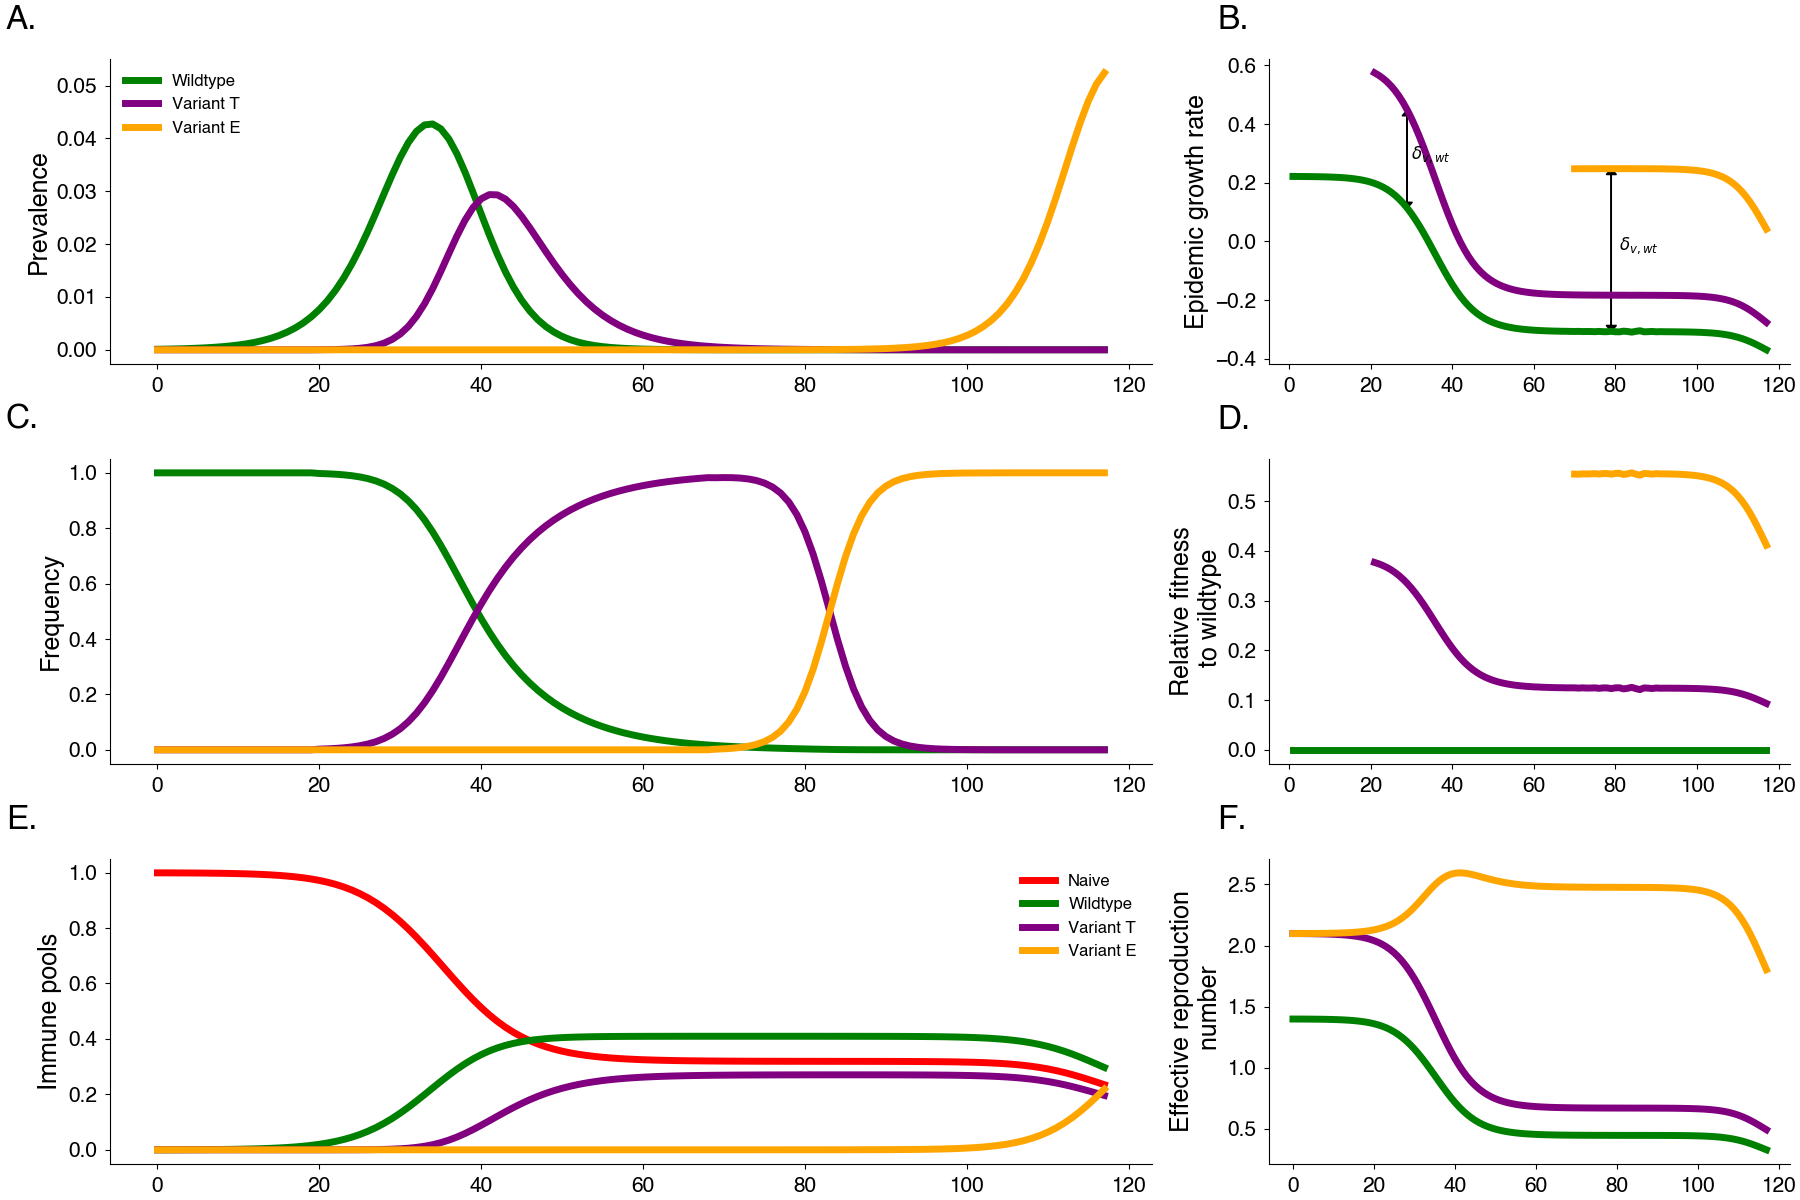
\includegraphics[width=1.0\linewidth]{./figures/vis_mechanisms.png}
    \caption{
      \textbf{Simulated variant dynamics in a mechanistic model.}
      Mechanistic transmission models constrain variant frequency dynamics by specifying a functional form for relative fitnesses.
      Simulations of a three-variant model including wildtype $W$, an intrinsic transmission variant $T$, and an immune escape variant $E$ show the relationship between population-level transmission and selection.
      We begin the simulation with initial wildtype prevalence $I_\wt(0) = 1$, effective reproduction number $R_{0,\wt} = 1.4$, and duration of infection $1/\gamma = 3.0$ days.
      We introduce transmissibility variant $T$ at $t=20$ with frequency $f_T(20) = 10^{-5}$ and a 50\% increase in transmissibility $\varTransmission_T = 0.5$.
      We introduce escape variant $E$ at $t=70$ with frequency $f_E(70) = 10^{-6}$ that infects 5\% of hosts possessing wildtype immunity $\varEscape_E = 0.05$.
      A. Prevalence $I$ by variant.
      B. Exponential growth rate $r$ by variant.
      C. Variant frequency $f$.
      D. Fitness relative to wildtype $\lambda$.
      E. Underlying immune pools.
      F. Effective reproduction number $R_t$ by variant.
      % \tbc{The axes labels of `Days', `Prevalence', etc...\ are a great size. However, you should slightly size up the the x and y tick labels of 0, 25, 50, etc...}
    }
    \label{fig:vis_mechanisms}
\end{figure}

% \subsection*{Estimating relative fitness using Gaussian Processes}

Our approach shows that relative fitness is often dependent on the past exposure of a population (as discussed in Supplementary Text \ref{ssec:frequency_dynamics}).
This suggests that serology, vaccination history, and immunological data generally can be informative of relative fitness.
Additionally, when working with variant classifications, non-neutral evolution within a variant will cause the relative fitness of that variant to change in time.
However, even in the absence of external data that can inform relative fitness, there is still hope.

We develop a method for using approximate Gaussian processes to model variant relative fitness.
Gaussian processes are probability distributions over functions, where the structure and smoothness of these functions are defined by a kernel that encodes correlations in time.
These models are flexible and allow us to encode smoothness constraints, periodicity, and other structures \cite{Gortler2019a}.
Gaussian processes allow us a non-parametric estimate of the relative fitness for variants through time (see Materials and Methods).

Traditional Gaussian process, while flexible, face challenges for large time series and large data sets.
Our approach overcomes this using a Hilbert Space Gaussian Process (HGSP) approximation, making the framework scalable for many variants and long time periods \cite{riutortmayol2022practical}.
This enables real-time variant fitness estimation and can be applied to any frequency data regardless of the underlying mechanism.
This model is used in Fig.~\ref{fig:gp_example} to estimate the relative fitnesses of different variants through time based on simulated variant sequence counts from frequencies shown in Fig.~\ref{fig:vis_mechanisms}.

Later, we apply this model to empirical SARS-CoV-2 sequence data from 50 US states and England from 2021 to 2022 to estimate relative fitness for variants circulating in that period, but first we continue analytic investigation into fitness dynamics.

\subsection*{Determining the transmisibility-escape tradeoff}

To understand the fitness trade-off between transmissibility and immune escape, we consider dynamics with a wildtype virus $\wt$ with $\varTransmission_\wt = 0$ and $\varEscape_\wt = 0$, an increased transmissibility variant $\varT$ with $\varTransmission_\varT > 0$ and $\varEscape_\varT = 0$ and an immune escape variant $\varE$ with $\varTransmission_\varE = 0$ and $\varEscape_\varE > 0$.

Following Equation \ref{eq:two_strain_relative_fitness}, we write relative fitnesses of the escape variant or transmissibility variant as
\begin{align*}
    \lambda_{\varE, \wt} &= \varEscape \beta \phi_{\wt}(t)\\
    \lambda_{\varT, \wt} &= \varTransmission \beta S(t).
\end{align*}

In the simplest case where individuals are either susceptible or have wildtype immunity ($S(t) + \phi_{\wt}(t) = 1$), we can compute the critical immune fraction $\phi^{*}$ at which $\lambda_{\varE, \wt}(\phi^{*}) = \lambda_{\varT, \wt}(\phi^{*})$ as
\begin{equation} \label{eq:critical_immunity}
    \phi^{*} = \frac{\varTransmission}{\varEscape + \varTransmission}.
\end{equation}

For past exposure level greater than $\phi^{*}$ escape variants have a higher relative fitness.
This trade off shows that increasing degree of escape entails that a lower proportion of past exposure is needed for escape variants to be preferred (Fig.~\ref{fig:transmission_tradeoff}).
Additionally, this shows that when intrinsic transmissibility increases are limited escape is more likely to be a dominant mechanism for variant turnover.

\begin{figure}[h]
    \centering
    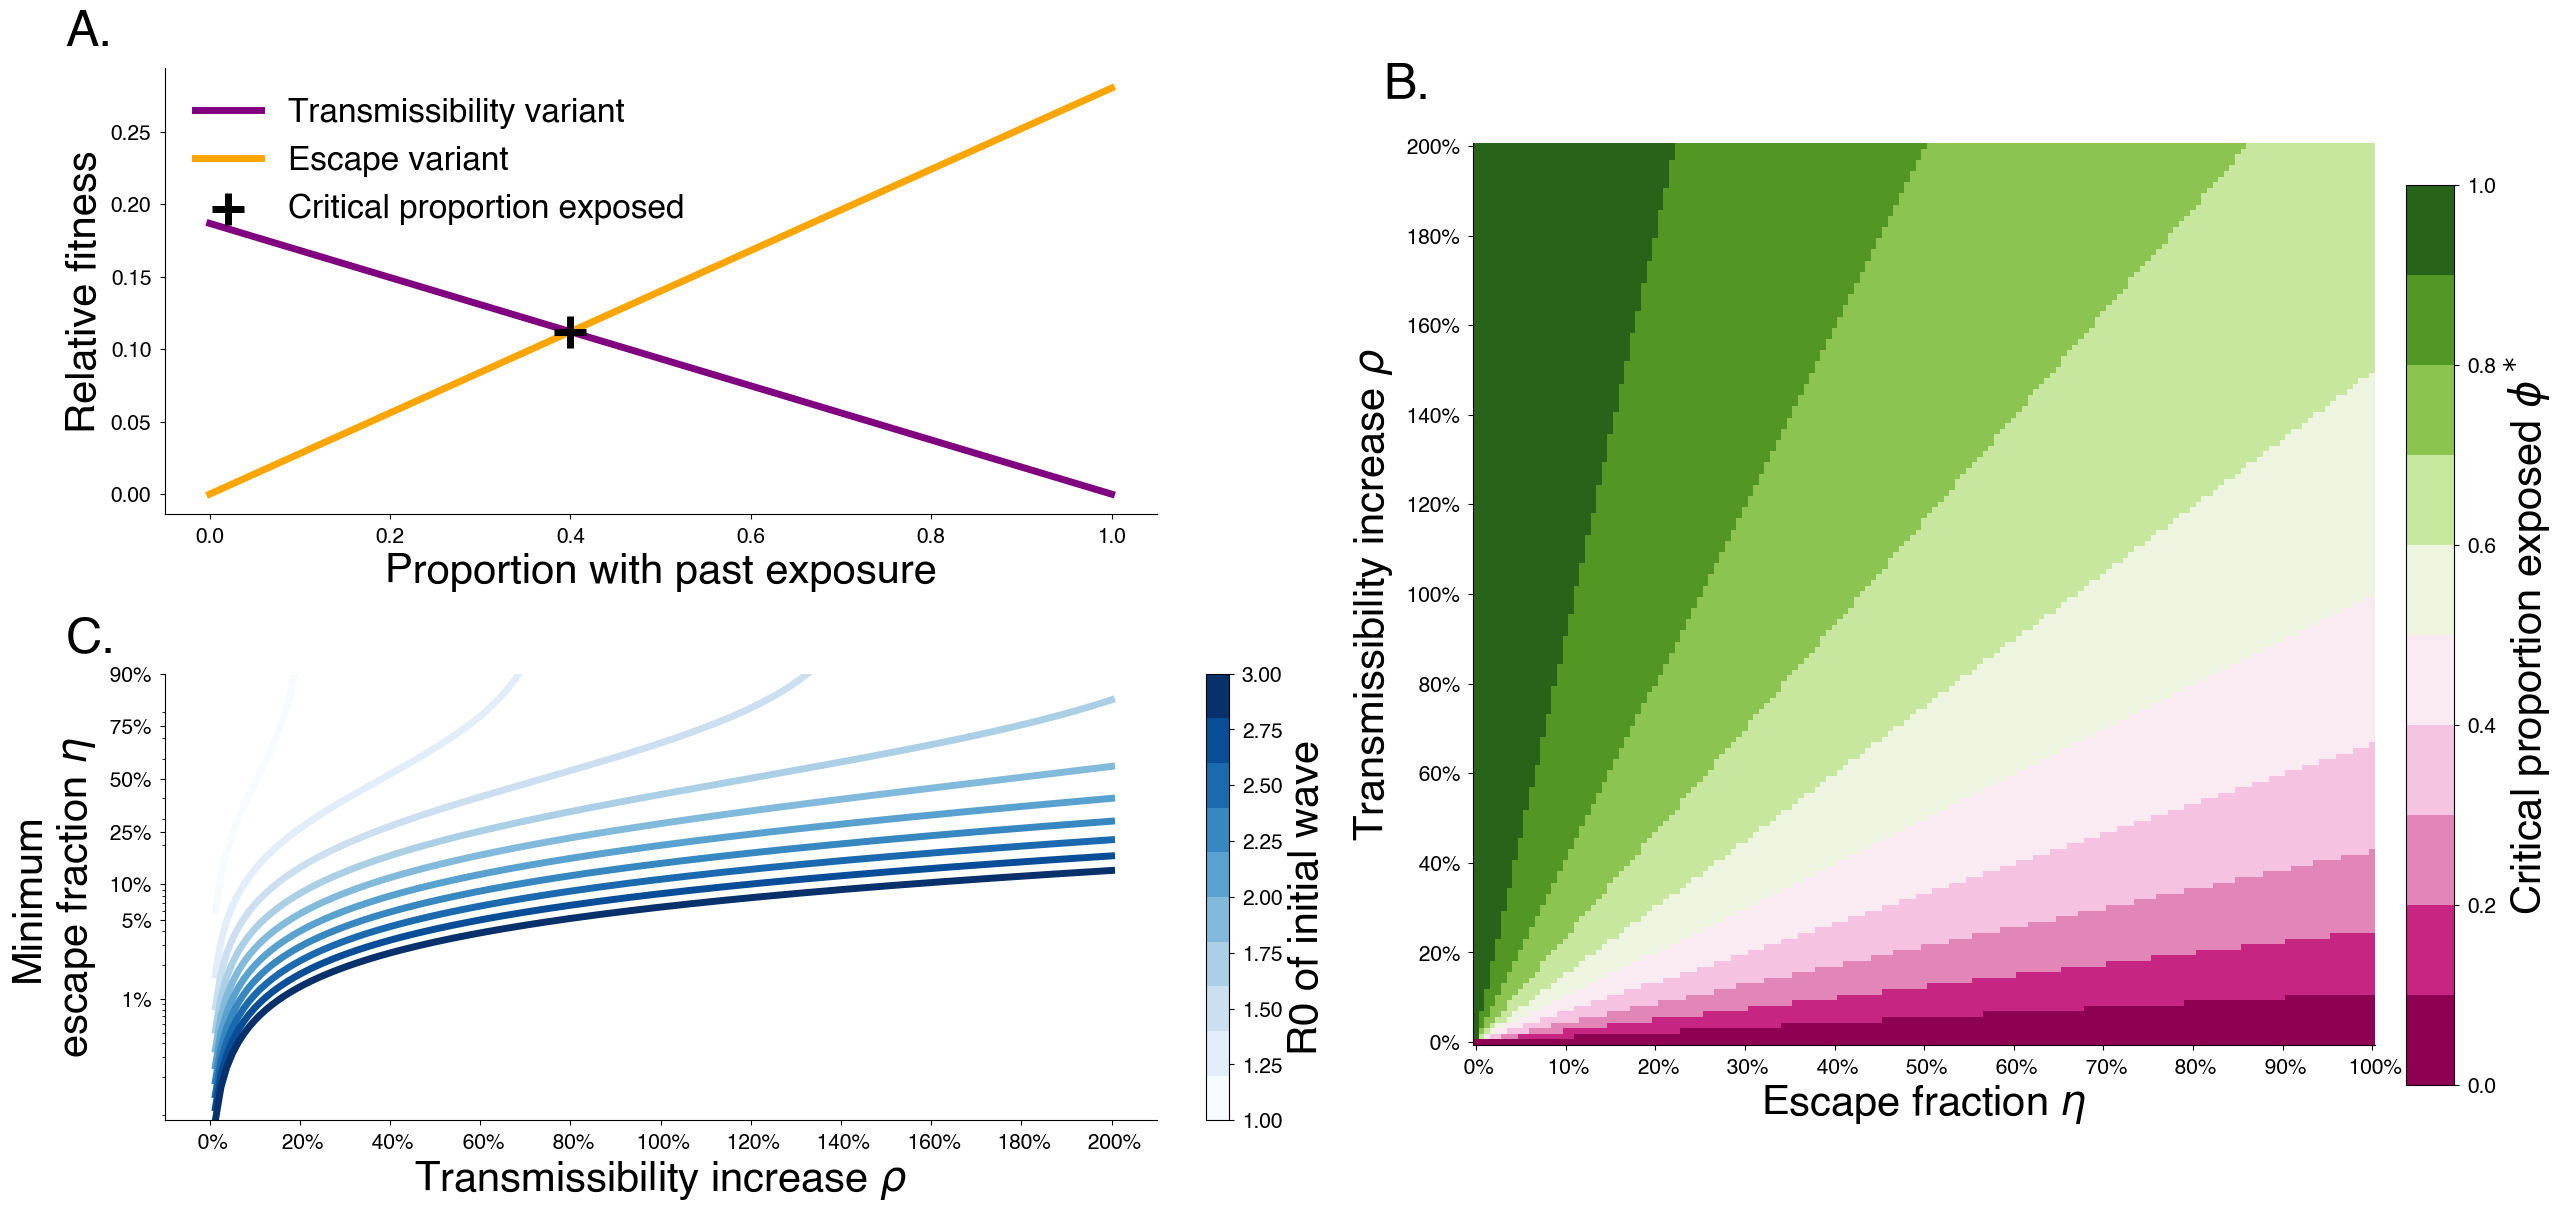
\includegraphics[width=1.0\linewidth]{./figures/transmission_tradeoff.png}
    \caption{
      \textbf{Trade-off between degree of immune escape and increased transmissibility.}
      A. Relative fitness for a transmissibility increasing variant $T$ with $\varTransmission_T=0.2$ and an immune escaping variant $E$ with $\varEscape_E=0.3$ for $R_{0, \wt}=2.8$ and $1 / \gamma = 3.0$ days.
      % \tbc{Fig.~\ref{fig:vis_mechanisms} uses $R_0$ instead of $\beta$. I do think $R_0$ is generally more interpretable and I'd swap $\beta$ for $R_0$ here unless for some reason $\beta$ matters in a way that $R_0$ does not.}
      % MF: I used $\beta$ here since that's what goes into the relative fitness calculation used here. Happy to switch to $R_0$ and $1 / \gamma$.
      The intersection point shows that after 40\% of the population has wildtype immunity, the escape variant has higher fitness.
      B. The critical exposure proportion is shown for various escape fraction and transmissibility increase. Above the critical exposure proportion, we expect dominance of escape variants.
      C. The minimum escape fraction needed for second waves to be comprised of escape variant assuming competition with transmissibility increase variants and first wave with a given $R_{0}$.
      % \tbc{I don't like the fact that in panels B and C you're showing $\varTransmission-1$ rather than $\varTransmission$. But I understand that you're doing so because it's more intuitive to start at zero. I'd propose to move from $\varTransmission \beta$ to $(1-\varTransmission) \beta$ throughout the text. This would bring $\varTransmission$ and $\varEscape$ in line with each other where 0 is equivalent to wildtype.}
      %MF: I've moved \rho -> 1 + \rho throughout. 
      % \tbc{Please attend to this in all figures, but I noticed it most obviously here. Currently legend and axes text is often too small. Even after I blew this up to 100\% page width the font on the x axis is 6pt or smaller. \tiny{Here's an example of 6pt for comparison.} \footnotesize{I prefer legends to be at least 8 pt as shown here.}}
    }
    \label{fig:transmission_tradeoff}
\end{figure}

\subsection*{Initial growth rates insufficient for predicting short-term frequency growth}

One question of interest is whether knowledge of mechanism meaningfully informs our ability to forecast short-term frequency growth.
The first step to addressing this is to understand how the relative fitness may change in time to understand the predictability of relative fitness in the short-term.

We find that the mechanistic forms analyzed in this paper (see Supplementary Text \ref{ssec:frequency_dynamics}) can be represented as weighted combinations of $B$ time-varying functions $\Upsilon_{b}(t)$ with weights $\beta_{b}$.
We can think of each of these functions $\Upsilon_b$ as an immune background and the coefficient $\beta_{b}$ as a transmission differential, so that
% TB: Shouldn't both of these be \Upsilon_b? Rather than the current "time-varying functions $\upsilon_{b}(t)$" and "these functions $\Upsilon_b$". I've made this change, but could be missing something.
\begin{align*}
\lambda_{v,u}(t) = \sum_{1 \leq b \leq B} \beta_{b} \Upsilon_{b}(t).
\end{align*}

Even in the case of complete knowledge of the relative fitness and the underlying fitness contributions in the present and past, we have that change in the relative fitness is determined by
\begin{align*}
    \frac{d\lambda_{v,u}}{dt} = \sum_{1 \leq b \leq B} \beta_{b} \frac{d\Upsilon_{b}}{dt}(t).
\end{align*}
By considering a Taylor expansion of the relative fitness about the point of estimation $t_{0}$, we can approximate the relative fitness in the future as:
\begin{align*}
    \lambda_{v,u}(t) \approx \lambda_{v,u}(t_{0}) + (t - t_0)\sum_{1\leq b \leq B} \beta_b \frac{d\Upsilon_b}{dt}(t_0).
\end{align*}
This suggests small differences in the form of $\lambda_{v,u}(t)$ can lead to meaningful differences in the future relative fitnesses through changes in the underlying immune backgrounds.

We investigate whether relative fitnesses vary predictably in the short-term regardless of mechanism.
To do so, we apply the two-variant model developed in previous sections for different mechanisms of immune escape and increased transmissibility.
We fix the relative fitness of the novel variant at a prediction time $t_{0}$ using Equation \ref{eq:critical_immunity} and assess the change in the relative fitness in the short-term.
We find that although relative fitness trajectories share the same decreasing shape, they may decline at different rates depending on the mechanism (Fig.~\ref{fig:short_term_divergence}).
This can lead to substantial changes in the predicted incidence depending on the assumed mechanism and affects to overall rate of turnover.

\subsection*{Correlations insufficient for mechanism identification}

Although correlations between vaccination uptake and variant growth advantage are often observed, these are alone may not be sufficient to identify the mechanism behind a variant's success.
A variant’s fitness advantage may arise from increased transmissibility, immune escape, or a combination of both.
Even in the absence of immune escape, the relative fitness of a variant depends on the proportion of the population that is susceptible to infection and therefore changes with both past exposure and vaccine uptake (Supplementary Text \ref{ssec:frequency_dynamics}).
To illustrate this, we simulate the spread of a variant with increased transmissibility in populations with varying initial vaccination levels.

In populations with lower vaccination levels, the variant’s prevalence peaks more sharply and its relative fitness declines quickly as immunity accumulates within the population (Fig.~\ref{fig:mechanism_identification}A-C).
In contrast, higher vaccination levels constrain relative fitness, leading to a delayed peak in prevalence and more stable relative fitness as the existing immunity limits the variant’s spread (Fig.~\ref{fig:mechanism_identification}A-C).
Even without immune escape, estimated growth advantages for this variant decrease with increasing vaccination uptake near the beginning of an epidemic (Fig.~\ref{fig:mechanism_identification}D).
Later in the epidemic, this relationship reverses with estimated growth advantages over the full period increasing with initial vaccination levels, which may be mistaken as signal for immune escape (Fig.~\ref{fig:mechanism_identification}E).
% At very high vaccination levels, we see the estimated growth advantage falls off sharply when both variants are declining in prevalence.
% This occurs at a critical vaccination threshold of $1 / R_v$ where $R_v$ is the effective reproduction number of the variant (Fig.~\ref{fig:mechanism_identification}E).

% This analysis shows a limitation in the ability of correlation-based analyses on growth advantage to identify the underlying mechanisms of variant fitness.
% By explicitly accounting for the dynamics of immunity and transmissibility within populations, incorporating epidemiological structure in these models might provide a good foundation for understanding variant success under assumed or scientific-motivated mechanisms and enable comparison between competing mechanisms.

This analysis shows that correlation-based methods alone may struggle to identify the true mechanisms driving a variant’s success especially under the assumption of a fixed growth advantage.
By explicitly considering how immunity and transmissibility interact within populations, models that incorporate these dynamics may provide a stronger foundation for understanding why certain variants spread.
% This approach also enables clearer comparison between different potential mechanisms behind variant fitness.

% Variant growth advantages can be correlated with vaccination proportions even in the absence of immune escape.
% Simulated multiple epidemics of a pure increased transmissibility variant at varying levels of initial vaccination and was able to see that estimated growth advantages, computed using a logit linear model, were correlated with initial vaccination fraction.
% We find that you can estimate association of increased relative fitness due to vaccination in the absence of immune escape (Fig.~\ref{fig:mechanism_identification}).
% This appears to hold up until both variants' initial effective reproduction number is below 1 i.e. $V_{0} > 1 / R_{v}$.

\begin{figure}[h]
    \centering
    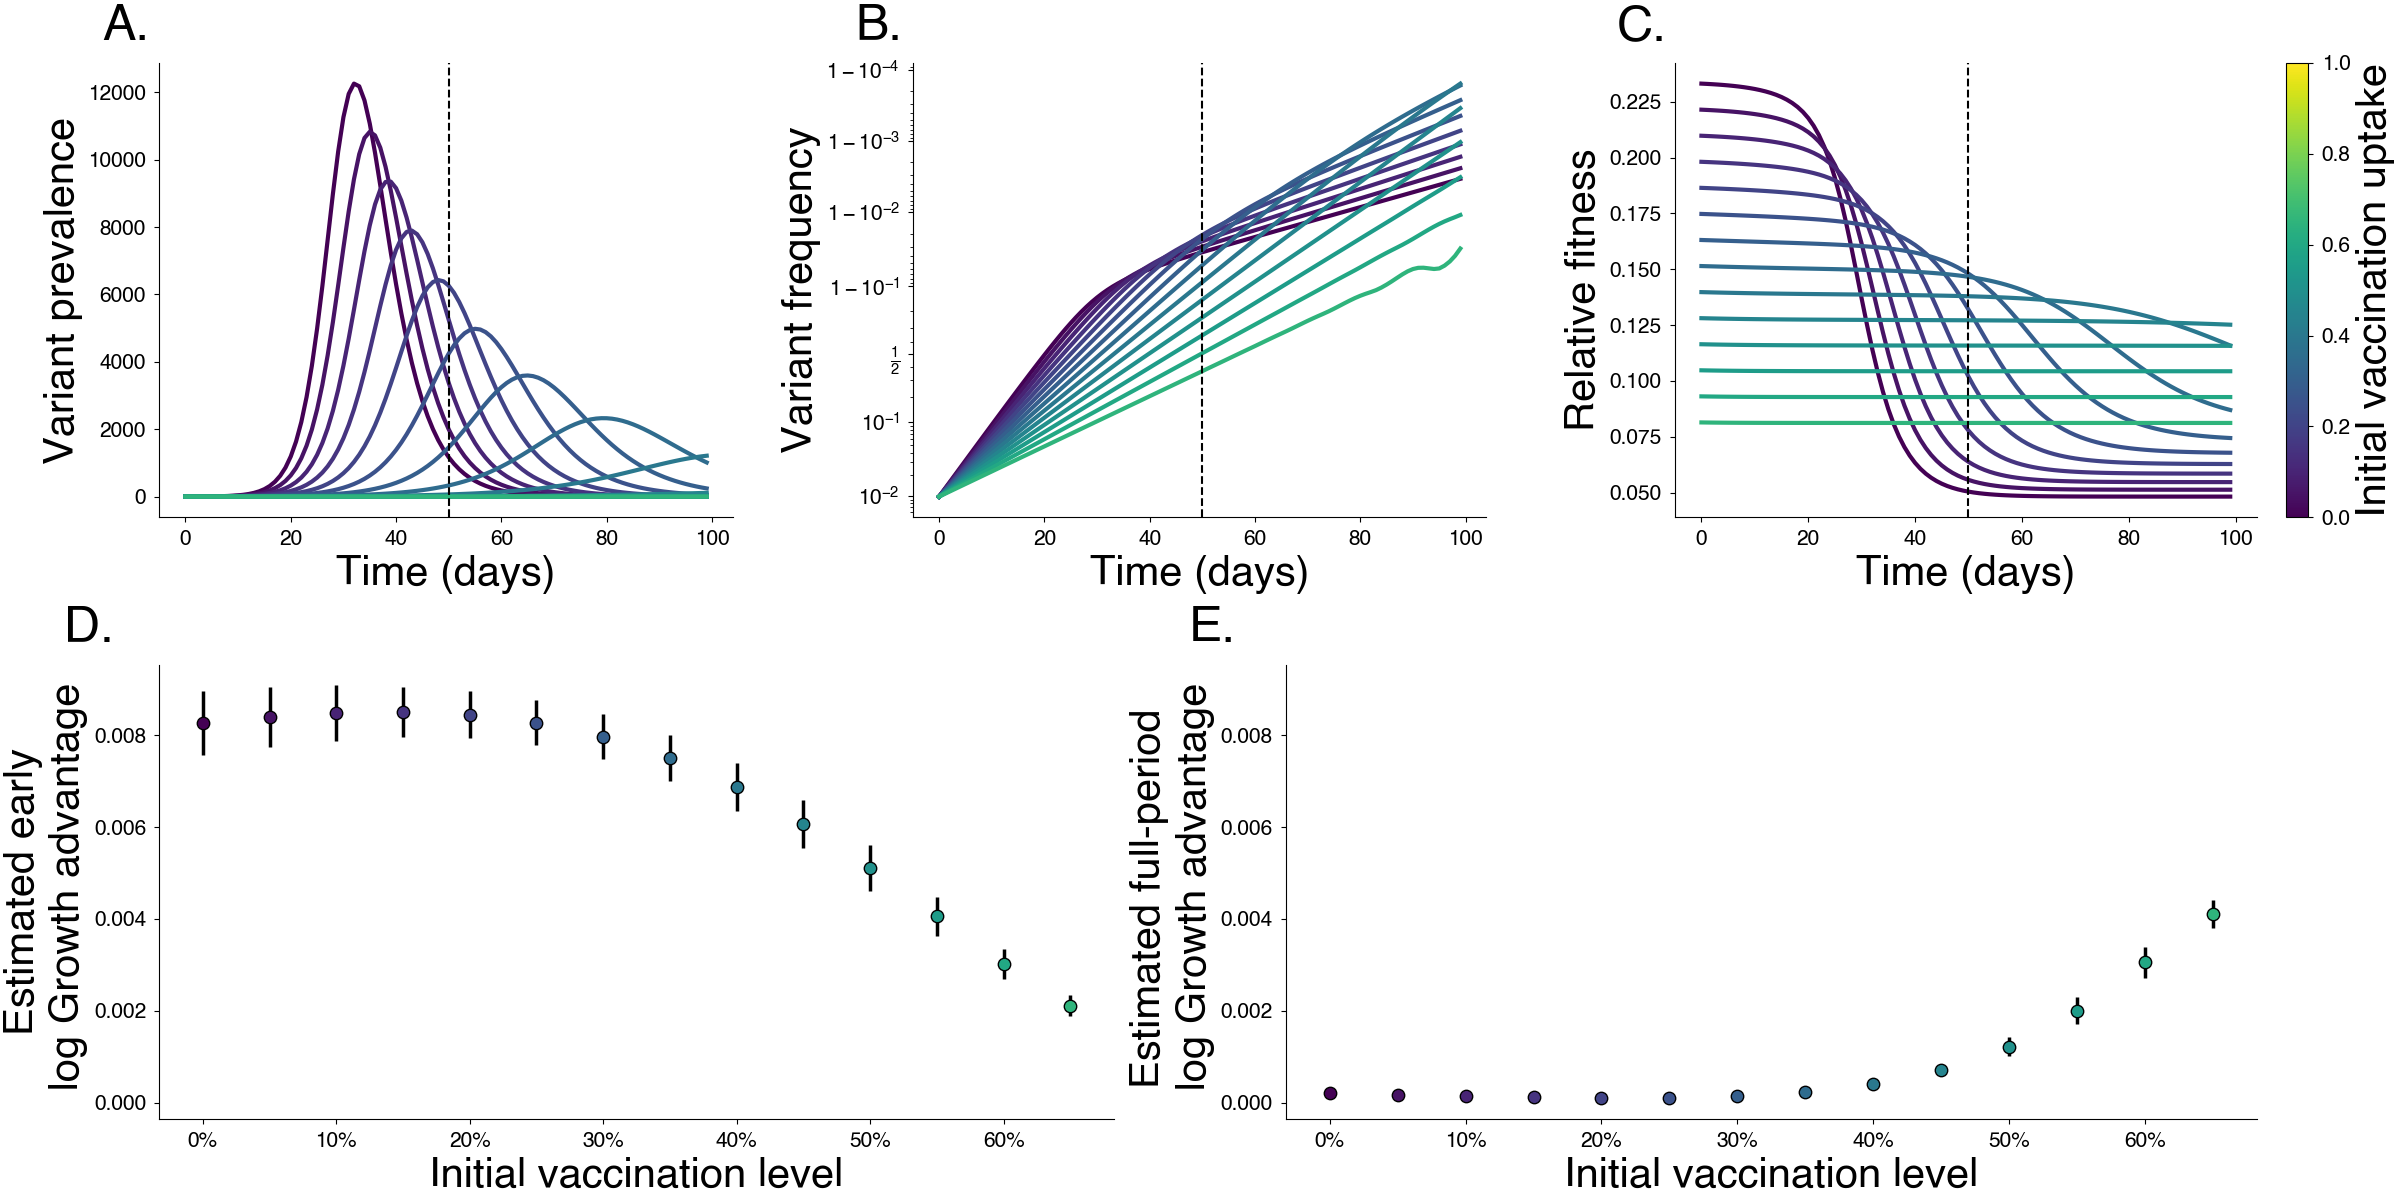
\includegraphics[width=1.0\linewidth]{./figures/mechanism_identification.png}
    \caption{
      \textbf{Relative fitness is correlated with vaccination levels in the absence of immune escape.}
      We simulate the growth of a pure transmissibility increased variant at varying levels of vaccination.
      Darker colors represent lower vaccine uptake.
      We identify an early growth period where relative fitness is at its highest; the cutoff for this period is denoted with a vertical dashed line.
      A. Prevalence of variant, each line is its own simulation.
      B. Frequency of variant.
      C. Relative fitness for variant over time.
      D. Estimated log growth advantage using linear regression of log relative frequency of variant over wildtype using only data before the early cutoff.
      E. Same as D. but using data from the entire period shown.
    }
    \label{fig:mechanism_identification}
\end{figure}

\subsection*{Quantifying selective pressure}

Although it is useful to quantify the relative fitnesses of individual variants, we are often interested in quantifying the overall effects of selection in the population.
With this in mind, we can derive a metric of overall selective pressure $\psi(t)$ which describes the distribution of relative fitness in the population
\begin{equation}
\psi(t) =  \Expect_{f(t)}\left[ \frac{d \lambda_v}{d t}\right] +  \Var_{f(t)}[\lambda_{v}].
\end{equation}
This selective pressure metric serves as an indicator for high fitness variants arising in the population as change.
High fitness variants rising from initially low frequency leads to large increases in the variance of the fitness distribution and therefore increases in the selective pressure.

The selective pressure metric enables us to decompose changes in the average growth rate in the population $d\bar{r}/dt$ to an evolutionary component $\psi$ and a residual baseline growth rate $r_\wt$ following
\begin{equation}
    \frac{d\bar{r}}{dt} = \frac{dr_{\wt}}{dt} + \psi(t).
\end{equation}
This shows that increased selective pressure through emerging high fitness variants can drive waves of infection.
Further, this suggests that differences between growth rates based on selective pressure alone and observed rates are attributable to changes in baseline transmission over time.
This mirrors ideas of Fisher's theorem of natural selection and its later interpretations with the variance of fitness contributing directly to the change in transmission rates (or fitness) \cite{Ewens1989, Ewens2024}.
This definition of selective pressure captures how relative fitness contributes to epidemic growth.
This is similar to ideas quantifying rates of adaptation via fitness flux \cite{Mustonen2010}.

In this case, the overall growth rate $\bar{r}$ and relative incidence $I(t) / I(0)$ can be written directly using the cumulative selective pressure $\Psi(t) = \int_0^t \psi(s)ds$ as follows:
\begin{align}
    \bar{r}(t) &= \bar{r}(0) + [r_{\wt}(t) - r_{\wt}(0)] + \Psi(t)\\
    \frac{I(t)}{I(0)} &= \exp \left( \int_0^t [r_{\wt}(s) + \Psi(s)]ds \right).
\end{align}
In addition to estimating the relative fitness, metrics derived from these models can be informative of much more.

Our ``selective pressure'' metric which allows us to model the contribution of evolution to changes in the epidemic growth rate of a population and is independent of pivot choice for relative fitness estimation.
This metric acts as an early warning system for variant-driven outbreaks, especially in scenarios where case data are sparse or delayed.
This metric can be computed using any method that estimates variant frequency and relative fitnesses and serves as a simple tool for understanding the contribution of selection to the overall population dynamics.
% This approach is compatible with any method which estimates frequency and relative fitness, enabling broad applicability to many pathogens.

The full derivation of this metric and its contribution to the overall growth rate can be found in Supplementary Text \ref{ssec:deriving_selective_pressure}.

\subsection*{Predicting epidemic growth rates using selective pressure}

Motivated by the relationship between epidemic growth rate and selective pressure demonstrated above, we develop a predictive model of epidemic growth rate using estimates of selective pressure.
% By integrating fitness estimates and variant frequency dynamics, selective pressure can be used to predict epidemic growth rates, empowering public health agencies to anticipate and respond to new variant-driven outbreaks.
Using empirical SARS-CoV-2 case and sequence data from 50 US states between January 2021 and November 2022, we estimate epidemic growth rates through time in each state using case counts, and estimate selective pressure through time using our approximate Gaussian process model on sequence counts  (Fig.~\ref{fig:selective_pressure_prediction} A--C.)
Here we group variants at the granularity of Nextstrain clades \cite{aksamentov2021nextclade} resulting in 37 distinct variants over this time period.
As expected we see that relative fitness increases through time and that selective pressure corresponds to speed of clade turnover where the sweep of Omicron BA.1 (clade 21K) yields the strongest signal of selective pressure (Figs.~\ref{fig:selective_pressure_group_1}--\ref{fig:selective_pressure_group_5}).
We use these estimates to fit a gradient-boosted regressor to predict epidemic growth rates using selective pressure from the most recent 28 days, reserving data between July 2022 and November 2022 for testing (Fig.~\ref{fig:selective_pressure_prediction} D--I, Fig.~\ref{fig:empirical_growth_rate_predictions_all}).
We observe a strong correpondence between observed epidemic growth rate and model predictions with Spearman correlation in the training period of $\rho = X$ and correlation in the testing period of $\rho = X$.
\tbc{Please fill in these values.}
\tbc{Currently Fig.~\ref{fig:growth_rate_predictions_model_comparison} is never referenced in the text. I believe you want to reference it here.}

We validate this method by testing this model to estimate epidemic growth rates in England derived from the Office for National Statistics (ONS) Coronavirus Infection Survey between February 2022 and November 2022.
The ONS Infection Survey represented a randomly sampled panel survey of households where nasal swabs were collected regardless of symptom status allowing for prevalence estimates despite faltering case reporting \cite{pouwels2021community}.
Our model is able to replicate patterns seen in epidemic growth rates in England derived from ONS data (Fig.~\ref{fig:selective_pressure_prediction} J--L), achieving a Spearman correlation of $\rho = 0.614$ and mean absolute error of 0.016 on per day epidemic growth rate.
% TB: I'm used to using \rho and not \rho^2 to report Spearman correlations
Performance is significantly better for the first two subsequent waves, falling off in accuracy for the fall 2022 BQ.1 (clade 22E) wave.

Although these predictions can be biased by non-evolutionary effects on the epidemic growth, this approach provides a simple measure of epidemic growth in the absence of high quality case counts using sequence data alone.

\begin{figure}[h]
    \centering
    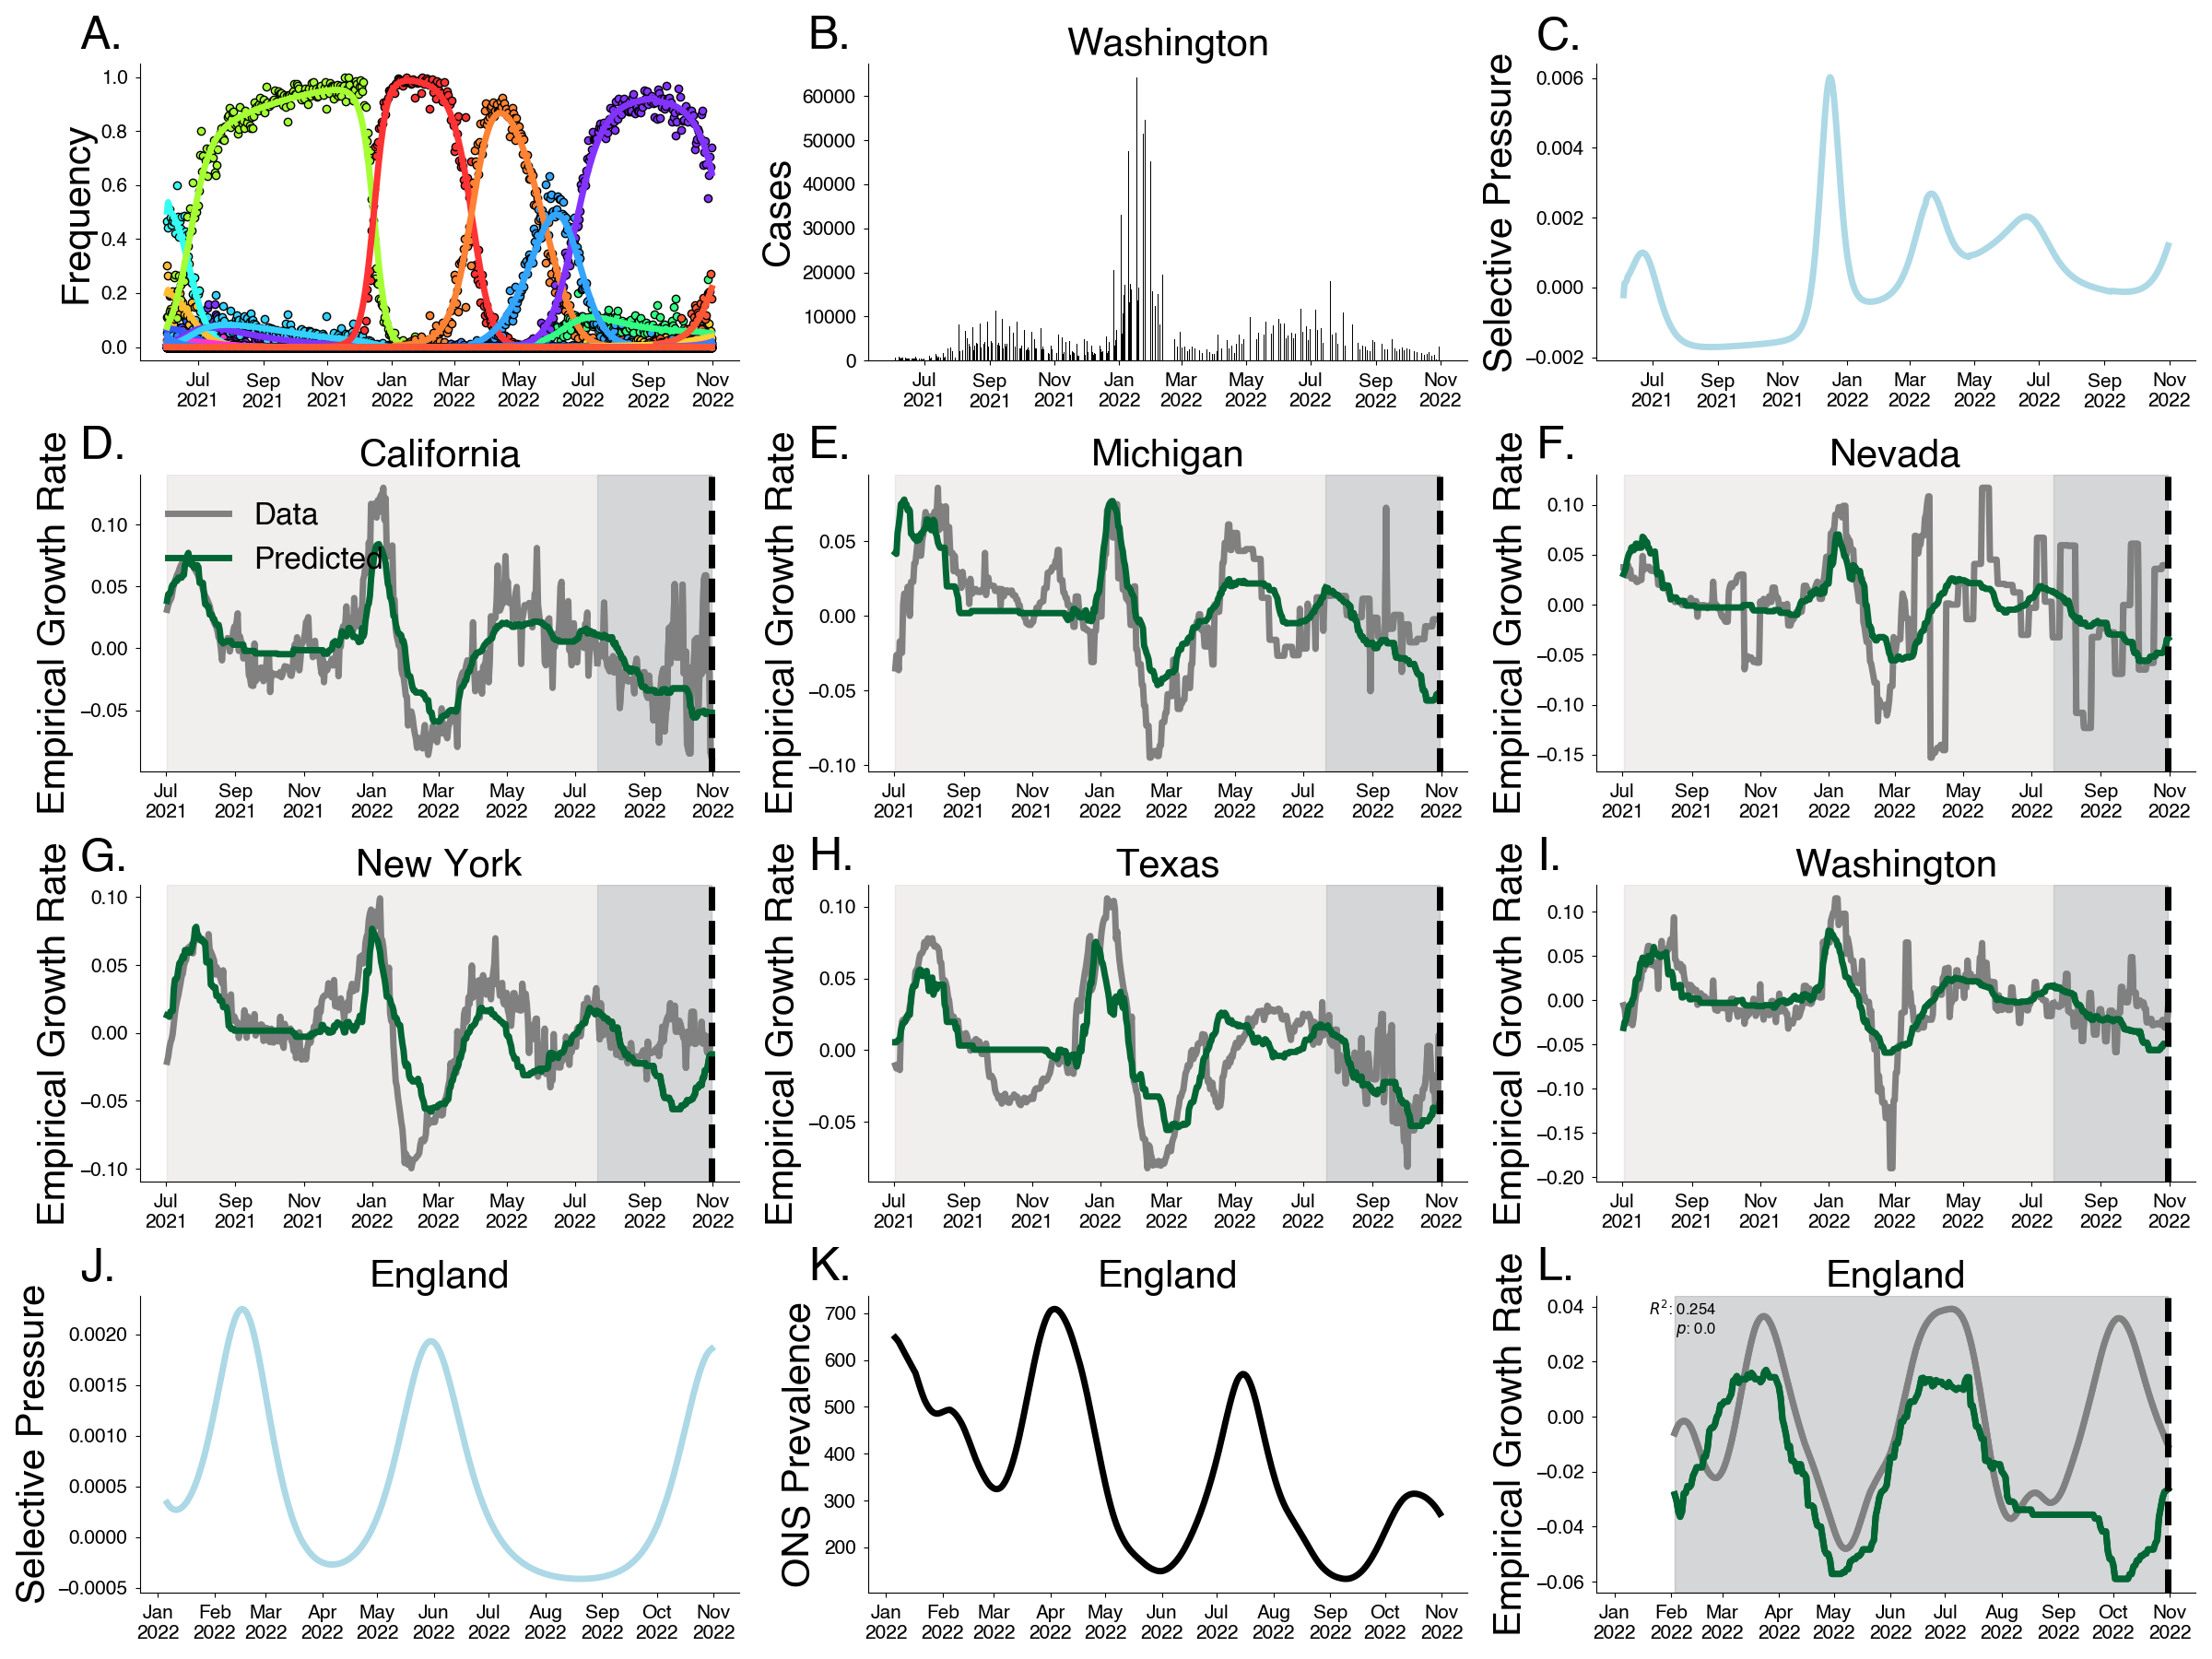
\includegraphics[width=1.0\linewidth]{./figures/selective_pressure_prediction.png}
    \caption{
      \textbf{Predicting epidemic growth rate using estimated selective pressure.}
      A. Variant frequency estimated using the Gaussian process relative fitness model between January 2021 and November 2022.
      B. Case counts from Washington state.
      C. Selective pressure computed using estimated variant frequencies and relative fitnesses from Washington state.
      D-I. Predictions for empirical growth rate from selective pressure for selected US states.
      The light gray period is the training period and the darker gray is the testing period.
      J. Estimated selective pressure in England.
      K. Prevalence estimates for England.
      \tbc{Please swap panels J and K to mirror panels B and C that are ordered as cases then selective pressure.}
      L. Empirical growth rates (gray) computed from prevalence estimates and predictions from our model (green) computed from selective pressure.
      \tbc{Again, I think the vertical dashed line can be dropped. It's not described in the caption and the darker background covers this anyway.}
    }
    \label{fig:selective_pressure_prediction}
\end{figure}

\subsection*{Latent factor model of relative fitness}

The representation of relative fitness using discrete immune backgrounds suggests that there may be low-dimensional structure to variant relative fitness.
To generate pseudo-estimates of this latent factors, we develop and implement our method for latent factors models of relative fitness.
This model assumes that variants intrinsically escape the immune responses with particular groups and that differences in a variant's relative fitness between geographies is attributable to differences in immunity between populations.
This enables us to estimate a pseudo-escape rates for variants (Fig.~\ref{fig:latent_immune}F) as well as pseudo-immunity groups within geographies over time (Fig.~\ref{fig:latent_immune}C).

% \tbc{Say more about what this model is and how it works intuitively (correlations in relative fitness between variants and countries). Keep equations / details in Methods and Supplemental Text.}

We generate Pango lineage-level sequence counts for 14 countries and 41 variants between March 2023 and March 2024.
These 14 countries were chosen based on availability of sequences.
Small lineages which do not meet a count threshold are collapsed into their parent lineages.
This leaves us with a total of 41 variants, so that each variant met a threshold for number of sequences available.

Using these sequence counts, we apply our latent factor model to estimate the relative fitness of each variant over time in each country, pseudo-escape rates for each variant, and pseudo-immunity for each country simultaneously for $D=10$ pseudo-immune groups.
Looking at the loss for the latent factor model for increasing $D$, we choose $D=10$ for our primary analysis by noting the point at which the loss function seems to stagnate with increasing $D$ i.e. the "elbow" method.
% \tbc{Make a comment of the size of immune space. Why five dimensions? If you haven't formally tested different dimensions you need to.}
%MF: Plan to add a replicate figueres with different K and then elbow plot showing the loss at different $K$.
The results of this model are visualized in Fig.~\ref{fig:latent_immune} for several selected variants and countries of interest.

% \tbc{This needs to be greatly expanded. Simply describe the results shown in Figure \ref{fig:latent_immune} and describe how you derive ``titer differences''. There's a whole lot going on here. Note things like the striped pattern in panel F where more closely related Pango lineages are assigned similar pseudo immune escape values without this being input into the model.}

Our results show that closely related Pango lineages are often assigned similar pseudo-escape values suggesting that this is capturing some evolutionary structure to immune escape.
Further, our model shows that these groups of lineages tend to target particular immune groups such as Clade 24A (JN.1, JN.1.1, JN.1.4) has high pseudo-escape in dimension 3.
If immune escape is the dominant mechanism for relative fitness difference, we expect that differences in immune response between variants from serological data would mirror differences in our pseudo-escape space.
Using human titer data from Jian et al, we compute titer distances as average log2 differences in titer values between pairs of variants. \cite{Jian2023} 
We, then, compare these distances to distances in our pseudo-escape space (Fig.~\ref{fig:latent_immune}G), finding the distances between distinct pairs in the pseudo-escape space are correlated with these titer differences between variants ($R^2$ = 0.26).
We bootstrap this analysis among 1,000 replicates to get a distribution among $R^2$ (Fig.`\ref{fig:latent_immune_bootstrap}).

 This approach can be applied to other rapidly evolving pathogens, such as influenza, making it broadly applicable beyond SARS-CoV-2.
 In fact, there is more utility for pathogens with larger geographic differences in immunity since this approach enables to estimate the proportion of these latent immune pools in the population and how they vary geographically and over time alongside variant difference.

By approximating antigenic differences using sequence data alone, this method offers for a deeper understanding of immune dynamics and how they shape variant success in the presence of immune escape.
This enables an embedding similar to those from antigenic cartography but without the need for serological data and based purely on observed variant fitness.

% \tbc{(More reviewer questions:) How does model fit of the latent factor model compare to the Gaussian process model from earlier in the text? Or is this applied after the Gaussian process estimates of relative fitness?}
%MF: This is a bit more difficult since this is a hierarchical model where the GP model is not.

\begin{figure}[h]
    \centering
    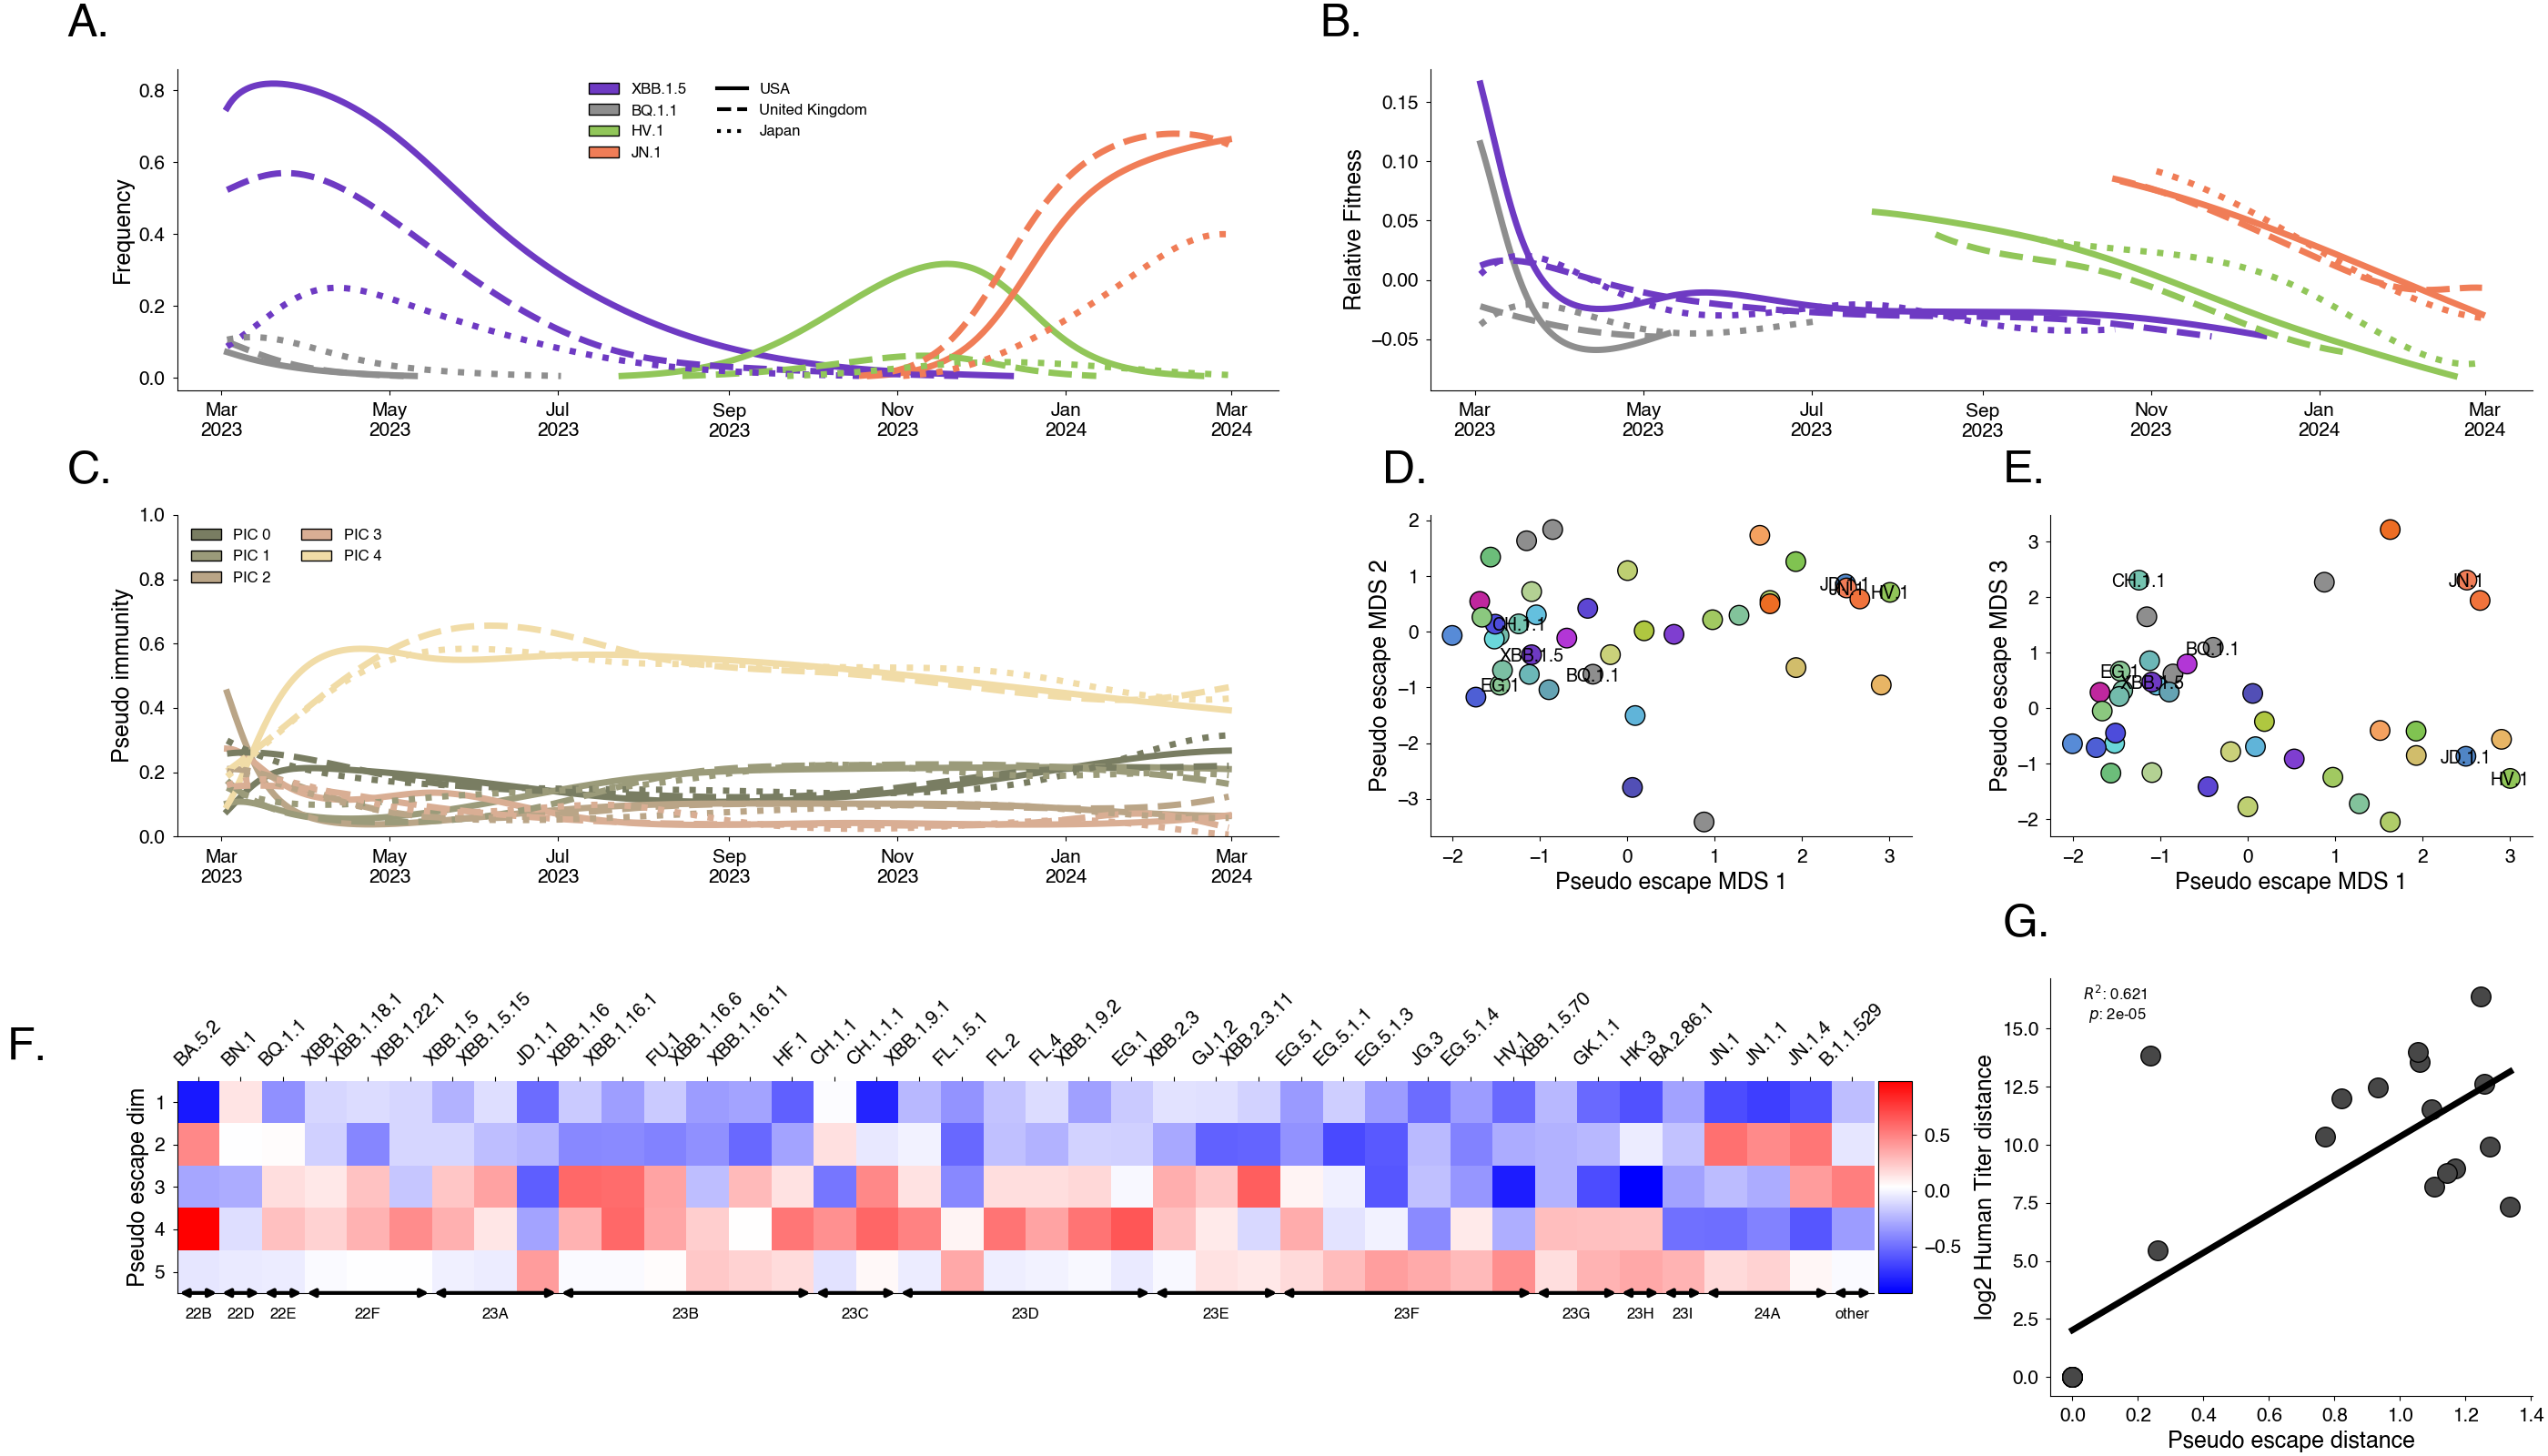
\includegraphics[width=1.0\linewidth]{./figures/latent_immune.png}
    \caption{
      \textbf{Latent factor models of immunity describe variant structure.}
      We fit the latent immunity factor model to recent SARS-CoV-2 sequence data globally.
      A. Variant frequency. Lines are colored by variant with the style of the line denoting countries of interest.
      % \tbc{Y axis in panel A should be 0\%, 20\%, etc...}
      B. Estimated relative fitness for selected variants and countries.
      % \tbc{Relative fitness to what? Note in the y axis label.} %MF: This is relative to other. Will add note to methods.
      C. Estimated pseudo-immunity over time for multiple countries.
      % \tbc{I read this as `principle component 1', etc... but I think these are directly immune pools. I suggest legend title of `Psuedo immune pools' over `Pool 1', `Pool 2', etc... swatches. Make this 1 to 5 and not current 0 to 4.}
      % \tbc{Order immune pools in a logical fashion in panels C and F and state what this ordering is based on.}
      %MF: They are already ordered and this is mentioned in the methods.
      D, E. Dimensionality-reduced pseudo-escape rates using Multidimensional Scaling.
      F. Estimated pseudo-escape rates for each variant.
      % \tbc{Why are there negative values here? I thought that pseudo-escape ranges from 0 to 1.}
      %MF: For identifiablity, these are difference relative to the pivot variant in terms of both transmission times escape potential, so it's fine and expected for them to be negative for some variants.
      H. Comparing distances in the pseudo-immune space C. to observed distances in human titer data.
    }
    \label{fig:latent_immune}
\end{figure}

% \subsection*{Overview of methods}
%
% \tbc{This whole ``Overview of methods'' section feels largely out of place in current Main Text setup. Main Text is effectively Results and Discussion. Things like the note on the latent factor model ``This is offers a tool for a deeper understanding of immune dynamics'' should immediately follow its presentation in the text. Same thing for ``Selective Pressure'' paragraph below. Please fold this text where it's not a restatement of what's already been said directly into the sections above. There should remain roughly a paragraph that becomes the start of the ``Conclusions'' section that's effectively the first two sentences here of ``Our study demonstrates...''.}
%
\subsection*{Conclusions, limitations, and future work}

Our study demonstrates the utility of multi-strain mechanistic models in interpreting variant frequency dynamics.
This enables a more detailed picture of variant success in environments with heterogeneous population immunity.

One key insight from this was the trade-off between intrinsic transmissibility increase and immune escape.
We showed that this trade-off is shifted by changes in population immunity, so that immune escape dominates as exposure increases.
Though there are limits to our ability to attribute dynamics to particular mechanisms from frequency data alone, the structure of these models suggests that we may improve forecasting by incorporating information about empirically supported mechanisms such as immune escape via antigenic evolution.

Despite these advances, there are limitations to our approach.
Long-term forecasts remain difficult, particularly as new variants with unknown fitness profiles emerge.
This framework suggests that considering both the escape against individual immune backgrounds and the diversity in human immune escape is most useful for improving forecasts of relative fitness.
Additionally, our models, while powerful in estimating short-term variant dynamics, rely on assumptions about transmission mechanisms that may not always hold across different pathogens or contexts.
In fact, as we've shown, it's entirely possible for shifts in population immunity to change the dominant transmission mechanism.

Furthermore, the models considered here are deterministic in nature and do not explicitly model the emergence of variant viruses only the dynamics after their successful introduction.
In reality, there are biological constraints on the types of variants that are produced in nature and even if there is a "true" fitness boost, the chance for stochastic extinction of beneficial variants remains.
These constraints present trouble for long-term forecasting as it will require a model of mutation or emergence, tying the potential for a variant to emerge with its potential to transmit in the current environment.
Future work should focus on improving the integration of real-time genomic data with serological and epidemiological data, providing a more comprehensive understanding of variant dynamics over time.

% These ideas are already represented in existing literature through the form of long-term forecast models which incorporate phylogenetic and molecular data which is thought to be indicative of selection and immune escape. \cite{Huddleston2020, luksza2014predictive}

% Future work should seek to identify and integrative informative data sources for relative fitness estimation and forecasting for particular pathogens, providing a more comprehensive understanding of variant dynamics over time.

% Limitations of existing simple mechanism models
% The compartment models discussed here are described by simple mechanisms and more work is needed to adapt this framework to complicated epidemic models such as those with non-exponential generation times could be useful.
% That being said, models which account for the appearance of genetic variants through mutation exist, often assuming a latent antigenic space with which fitness is determined.
%
% However, it is important to note that these models may not be reliable for longer terms forecasts due to the emergence of new variants or improper specification of mechanism.

% Despite the limitations discussed above, the framework presented here illustrates the importance of transmission mechanism in the evolution of pathogens, highlighting the importance of both variant characteristics and population susceptibility in selection.
% We suggest that future models of pathogen transmission and evolution attempt to incorporate current knowledge of the transmission process into their forecasts.
% In particular, for viruses such as influenza and SARS-CoV-2 which undergo antigenic evolution, our work suggests that incorporating knowledge on both the diversity in human immune response and the escape potential of emerging variants could prove useful in improving long-term forecasts of the viral population.

In conclusion, our framework represents a significant advance in our understanding of viral evolution and transmission dynamics.
By linking variant fitness to specific transmission mechanisms, we provide a more nuanced and accurate prediction of how variants will spread and impact population-level epidemic growth.
The selective pressure metric and latent immunity model offer new tools for public health agencies to monitor viral evolution in real time, enabling proactive intervention and insight into the variant difference and wave potential.
While our work has been applied to SARS-CoV-2, the methods developed here are broadly applicable to other evolving pathogens, offering a versatile approach for improving epidemic forecasting, variant monitoring, and overall pandemic preparedness.

\subsection*{Acknowledgements}

We thank Ivana Bozic, Betz Halloran, Mark Kot and Erick Matsen, as well as members of the Bedford Lab for their feedback on this work.

\subsubsection*{Funding}

This work is supported by NIH NIGMS award R35 GM119774 to TB and a Howard Hughes Medical Institute COVID-19 Collaboration Initiative award to TB.
MDF is an ARCS Foundation scholar and was supported by the National Science Foundation Graduate Research Fellowship Program under grant No.\ DGE1762114.
TB is a Howard Hughes Medical Institute Investigator.

\subsubsection*{Author contributions}
MF conceived the study.
MF, TB gathered sequence and case count data.
MF designed and implemented the models.
MF performed the analysis.
MF, TB interpreted the results.
MF, TB wrote the paper.

\subsubsection*{Competing interests}

All authors declare no competing interests.

\subsubsection*{Data and materials availability}

Source code used to generate figures, model implementations, and sequence count data are available at \href{https://github.com/blab/relative-fitness-mechanisms}{github.com/blab/relative-fitness-mechanisms}.

\bibliographystyle{plos}
\bibliography{relative-fitness-mechanisms}

\newpage

\appendix

\setcounter{figure}{0}
\setcounter{table}{0}
\setcounter{page}{1}
\renewcommand{\thefigure}{S\arabic{figure}}
\renewcommand{\thetable}{S\arabic{table}}
\renewcommand{\thepage}{S\arabic{page}}
\renewcommand{\thesubsection}{S\arabic{subsection}}

\begin{center}\Large
Supplementary Information for \\
\bf Frequency dynamics predict viral fitness, antigenic relationships and epidemic growth
\end{center}

\section*{Materials and Methods}

\paragraph{Generating sequence counts}

We prepared sequence count data sets using the Nextstrain-curated SARS-CoV-2 sequence metadata \cite{Hadfield2018} which is created using the GISAID EpiCoV database \cite{khare2021gisaid}.
These sequences were tallied according to either their annotated Nextstrain clade or Pango lineage depending on the data set to produce sequence count for each variant, for each day over the period of interest, and in each location analyzed \cite{aksamentov2021nextclade}.


\paragraph{Likelihood of sequence counts given frequencies}

The models discussed in this paper use counts of variant sequences to inform the underlying variant frequency in the population.
This is accomplished using a multinomial likelihood, so that given counts of sequences $C_{t,v}$ of variant $v$ at time $t$ and total sequences $N_{t}$ collected at time $t$, we have that

\begin{equation*}
    C_{t, \cdot} \sim \text{Multinomial}(N_{t}, f_{v}(t)),
\end{equation*}

where $f_{v}(t)$ is the frequency of variant $v$ at time $t$.
This is a simple model of sequence counts to frequencies and does not account for over-dispersion of sequence counts relative to a multinomial, however, all models can be extended to estimate and account for over-dispersion by replacing the above likelihood with a Dirichlet-Multinomial likelihood.

\paragraph{Approximate Gaussian processes for relative fitness estimation}%

To generate smooth non-parametric estimates of variant growth rates, we develop a Gaussian process based model for relative fitnesses.
That is, we model the relative fitness for each variant $v$ over time as a multivariate normal distribution:

\begin{align*}
    \vec{\lambda}_{v} &\sim \text{Normal}(\vec{\mu}, \vec{\Sigma})\\
    \vec{\Sigma}_{s, t} &= K_{\theta}(s, t),
\end{align*}
where $K_{\theta}$ is a potentially parameterized kernel function.
This induces a structure on the covariance of the relative fitness values over time.


For computational efficiency, we implement a Hilbert Space Gaussian Process (HSGP) approximation instead of fitting $V$ independent Gaussian processes.
This approximation allow us to share basis functions between variants \cite{riutortmayol2022practical}.
Under this approximation, the relative fitnesses are computed as

\begin{equation}
    \lambda_{v}(t) \approx \sum_{j=1}^{m} S_{\theta}(\sqrt{\mu_{j}})^{1/2} \cdot \phi_{j}(t) \cdot \beta_{j},
\end{equation}
where $S_{\theta}$ is the spectral density of the kernel $K_\theta$, $\mu_{j}$ and $\phi_{j}$ are the eigenvalues and eigenfunctions of the Laplacian, and $\beta_{j} \sim \text{Normal}(0,1)$ \cite{riutortmayol2022practical}.
Since the eigenvalues and eigenfunctions are shared across variants, this allows us to re-use values across variants, simplifying the computation to a matrix multiplication as

\begin{equation*}
    \vec{\lambda}_{t} = \vec{\Phi}_{t} \sqrt{\vec{S}_{\theta}}\vec{\beta}.
\end{equation*}

For the analyses in this paper, we use this approximate Gaussian process with a Mat\'ern 5/2 kernel and shared hyperparameters across variants.
We use this model to estimate relative fitnesss for the simulated data in Fig.~\ref{fig:vis_mechanisms} which are visualized in Fig.~\ref{fig:gp_example}.

\paragraph{Correlations are insufficient for mechanism identification}


To assess how vaccination uptake affects the growth advantage of a variant with increased transmissibility, we simulated the spread of a more transmissible variant across populations with different initial past exposure and vaccination levels.
This enabled us to isolate the effects of transmissibility within different immunity landscapes, examining how relative fitness and growth advantage shift based on population vaccination coverage alone in the absence of immune escape.
We begin with the 2-variant SIR model described in Supplemental appendix \ref{ssec:frequency_dynamics}.
We simulate this model for 100 days generation time $\tau = 1 / \gamma = 3.0$ days, $R_{0}^{\wt} = 1.4$ with $I_{\wt}(0) = 100$, $I_v(0) = 1$ and a 50\% transmissibility increase ($\varTransmission=0.5$) and no immune escape ($\varEscape=0.0$).
We divide the period into early and late epidemic with the breakpoint being $t=50$.
In Fig.~\ref{fig:mechanism_identification}D-E, we estimate the log Growth advantage for the variant in the early and full periods using a logit-linear model:

\begin{equation*}
\log \left( \frac{f_v(t)}{1 - f_v(t)} \right) = \beta t / \tau + \alpha,
\end{equation*}
where we take the model slope $\beta$ to be our log growth advantage.

We repeat these simulations for a range of vaccination levels starting from 0\% and ending at 65\%.

\paragraph{Predicting epidemic growth rate from selective pressure}%

The derivation of the selective pressure metric shows that the selective pressure can be a useful tool in predicting the epidemic growth rate.
To develop a predictive model of epidemic growth rate using selective pressure, we begin by generating estimates of selective pressure and epidemic growth rate from a period with high sequencing and case surveillance.

We take sequence count and case count data from all states in the United States between January 2021 and November 2022.
Using the sequence counts, we compute selective pressure estimates from relative fitness and frequencies estimated with our approximate Gaussian process relative fitness model.

From the case data, we derive the empirical growth rate using a 14-day moving average on case counts $\hat{C}_{t}$ and computing the empirical growth rate as $\hat{r}_{t} = \log(\hat{C}_{t}) - \log(\hat{C}_{t-1})$.

We then use the past 28 days of selective pressure to predict the empirical growth rate.

We use a gradient boosting regressor model with 100 estimators and max tree depth of 5 which is fit using a mean absolute error loss function.
This model was selected as it achieved the minimal error via time series cross-validation averaged across 5 splits among candidate models.
The candidate models include linear regression, ridge regression, Lasso regression, random forests, and gradient-boosted trees as implemented in scikit-learn \cite{scikit-learn}.

We validate our model by comparing our predicted epidemic growth rates to estimates of the epidemic growth rates in England derived from ONS data between January 2022 and September 2022 as well as to held-out testing data for US states.

\paragraph{Latent immune factor model}%

We show that relative fitness dynamics ought to be explained by low-dimensional immunity when transmission dynamics are described with compartment models.
This motivated a model to learn this low-dimensional structure that is inspired by latent-factor models.
We start by assuming that the relative fitness of variant $v$ at time $t$ and in geographic location $g$ can be described by $D$ latent factors so that

\begin{equation}
    \lambda_{v}^{g}(t) = \sum_{d=1}^{D} \varEscape_{v,d} \phi_{d}^{g}(t).
\end{equation}
As the structure here resembles Equation~\ref{eq:escape_relative_fitness}, we call the $\varEscape$ ``pseudo-escape'' and $\phi_{d}^{g}$ the ``pseudo-immunity''.
To make this more consistent with our intuition here, we model $\phi_{d}^{g}$ to be in $[0,1]$ and model it as smoothly varying in time.
In the results shown above, we model $\text{logit}(\phi_{d}^{g})$ using 4th order splines with 6 knots placed uniformly over the time period modeled.
Though we choose to model these latent factors with splines, other models would work here.
For example, one alternative would be the approximate Gaussian processes described above.
Additionally, in order to ensure identifiability of the parameter estimates, we fix some base variant $v^*$ which fitness is defined relative to, so that $\varEscape_{v^*, d} = 0$ for all $1\leq d\leq D$.
For the same reason, we fix the order of components, so that the components are numbered in decreasing order by their share in the first geography.

We apply this model to SARS-CoV-2 sequence counts in the period between March 2023 to March 2024 for 14 countries.
To access the necessary number of immune dimensions, we vary the number of immune dimensions between $D=2$ to $D=12$.
Looking at the loss for the latent factor model for increasing $D$, we choose $D=10$ for our primary analysis by noting the point at which the loss function seems to stagnate with increasing $D$ i.e. the "elbow" method (Fig.~\ref{fig:latent_factor_dimension}).

We compare the distances between variant pairs in our estimated pseudo-escape space to distances in log2 titer.
Using human titer data, we compute titer distances as the average log2 differences in titer values between pairs of variants for individuals.
This analysis is repeated among 1,000 bootstrapped samples to create a distribution of $R^2$ values (Fig.~\ref{fig:latent_immune_bootstrap}).
Additionally, we subset this by exposure history and repeat this analysis to find which exposure groups best explain distances in pseudo-escape space (Fig.~\ref{fig:titer_distance_correlations_by_group}).

\subsection*{Data and code accessibility}

Source code used to generate figures, model implementations, and sequence count data are available at https://github.com/blab/relative-fitness-mechanisms.

\newpage

\section*{Supplementary Text}

\tbc{It would be good if each of these sections S1, S2 and S3 were explicitly referenced in the Main Text or Materials and Methods. Ideally a reader is working through the Main Text / Methods and knows when it's most appropriate to read section S1, etc...}

\subsection{Exponentially growing populations to frequency dynamics}\label{ssec:frequency_dynamics}

We consider a viral population consisting of $V$ exponentially-growing variant viruses each with prevalence $I_{v}$.
Defining the time-varying growth rate for the prevalence of variant $v$ as $r_{v}(t)$, we can represent the prevalence using the following ordinary differential equation:

\begin{equation} \label{eq:inhomo_exp_growth}
    \frac{d I_{v}}{d t} = r_{v}(t) I_{v}(t), \quad v = 1,2, \ldots, V.
\end{equation}

The above differential equation has a known solution in terms of the integral of the time-varying growth rate and initial prevalence as follows:

\begin{align*}
I_{v}(t) = I_{v}(0) \exp\left( \int_{0}^{t} r_{v}(s) ds\right),
\end{align*}
where $I_{v}(0)$ is the initial prevalence of variant $v$.

Now turning to the frequency dynamics of the population, we write the frequency of variant $v$ in the population as  $f_{v}(t) = I_{v}(t) / \sum_{u=1}^{V} I_{u}(t)$.
This allows us to derive an ODE for variant frequency in terms of the variant growth rates using the quotient rule for differentiation:
\begin{align*}
    \frac{d f_{v}}{d t} &= f_{v} \left( \sum_{u=1}^{V} [r_{v}(t) - r_{u}(t)] f_{u} \right)\\
                        &= f_{v} \left( r_{v}(t) - \sum_{u=1}^{V} r_{u}(t) f_{u} \right).
\end{align*}

This system of differential equations resembles a logistic growth equation and can be shown to have the following solution in terms of the initial frequencies $f_{v}(0)$ and the variant growth rates:
\begin{align}
    f_{v}(t) &= \frac{ f_{v}(0) \exp( \int_{0}^{t} r_{v}(s) ds)}{\sum_{u=1}^{V}  f_{u}(0) \exp( \int_{0}^{t} r_{u}(s) ds)}.
\end{align}

The above representation of the variant frequency will serve as a centerpiece for many of the arguments to follow.
We see that by tracking the rate at which variant viruses are spreading, we can construct the corresponding frequency dynamics without knowing the absolute prevalence of any variant.

\paragraph{Relative frequency and relative fitness}%

Using the above equation for the variant frequencies, we can write the relative frequency of variant $v$ over $u$ as $x_{v,u}(t) = f_{v}(t) / f_{u}(t)$ to see:
\begin{align*}
    x_{v, u}(t) = \frac{f_{v}(t)}{f_{u}(t)} &= \frac{f_{v}(0)}{f_{u}(0)} \exp \left( \int_{0}^{t} [r_{v}(s) - r_{u}(s)] ds \right)\\
                                            &=x_{v,u}(0)\exp \left( \int_{0}^{t} \lambda_{v,u}(s) ds \right).
\end{align*}

Notice this relative frequency change depends on the initial relative frequencies and the \emph{relative fitness} $\lambda_{v,u}(t) = r_{v}(t) - r_{u}(t)$ of $v$ over $u$.
This relative fitness has the same units as the exponential growth rate (e.g. per day).
Using the definition of relative fitness, we can notice that
\begin{align}
\lambda_{v, u}(t) = r_{v}(t) - r_{u}(t) = \frac{d }{d t} \left[\log \left( x_{v,u}(t) \right) \right] = - \lambda_{u,v}(t)
\end{align}

We can see that there is a symmetry in the relative fitnesses and that the associated frequency dynamics depend on the differences between relative fitnesses.
This suggests that absolute fitness (in terms of the growth of infections) may not be inferable from frequencies alone.
This definition of relative fitness becomes essential in describing various existing modeling approaches for frequency dynamic data and motivates possible extensions since we can represent these models as having the form:
\begin{align}
    f_{v}(t) &= \frac{ f_{v}(0) \exp( \int_{0}^{t} \lambda_{v, \text{pivot}}(s) ds)}{\sum_{u=1}^{V}  f_{u}(0) \exp( \int_{0}^{t} \lambda_{u, \text{pivot}}(s) ds)},
\end{align}
where the growth rate of $v$ is expressed as relative to an arbitrary pivot variant.

\paragraph{Cumulative relative-fitness and frequency change}

Above we saw that within our framework frequency change over time intervals depends only on the cumulative relative fitness over time intervals $\Lambda_{v,u}(0, t) = \int_{0}^{t} \lambda_{v, u}(s)ds$.
We can then characterize approaches for modeling frequency change in terms of how they represent, estimate, and forecast these relative fitnesses.
This framework includes various existing methods for analyzing frequency data such as the seasonal influenza forecasting models of L{\"a}ssig and {\L}uksza \cite{luksza2014predictive} and Huddleston et al \cite{Huddleston2020}, multinomial logistic regression for frequency estimation \cite{Annavajhala2021} and the SARS-CoV-2 mutational fitness model of Obermeyer et al \cite{Obermeyer2022}.
%Question: How would I nest Piantham in this framework? Can I?

Though this framework can be used to describe existing statistical methods for frequency modeling, it is also applicable to traditional compartmental models of epidemics.
In fact, applying these ideas to compartmental models enables to see how mechanistic assumptions on the transmission process determine relative fitness of variant viruses.

\paragraph{Two-strain SIR}%

For simplicity, we will begin by analyzing a two-strain SIR model in which a variant virus $v$ can differ from wildtype virus wt by increased intrinsic transmissibility (via $\varEscape_{T}$) and immune escape against wild-type immunity (via $\varEscape_{E}$).
This system of 5 ordinary differential equations follows

\begin{align*}
    \frac{d S}{d t} &= - \beta S I_{\wt} - \beta \varTransmission S I_{v}\\
    \frac{d I_{\wt}}{dt} &= \beta S I_{\wt} - \gamma I_{\wt}\\
    \frac{d I_{v}}{dt} &= \beta (1+\varTransmission) S I_{v} + \beta (1+\varTransmission) \varEscape \phi_{\wt} I_{v} - \gamma I_{v}\\
    \frac{d \phi_{\wt}}{dt} &= \gamma I_{\wt} - \beta (1+\varTransmission) \varEscape \phi_{\wt} I_{v}\\
    \frac{d \phi_{v}}{dt} &= \gamma I_{v}.
\end{align*}
where $I_{\wt}$ denotes wild-type prevalence, $I_{v}$ denotes variant prevalence and $\phi_{\wt}$ denotes immunity derived from wild-type infection.
In this model, the variant virus can infect both susceptible individuals $S$ and individuals with immunity to wild-type virus $\phi_{\wt}$.
Increased intrinsic transmissibility increases the baseline transmission rate from $\beta$ in wild-type to $\beta \varTransmission$ in the variant virus and immune escape increases the transmission rate against those with wildtype immunity, so that the at-risk population is $\varEscape \phi_{\wt}$.

Writing that $r_{\wt}(t) = \beta S - \gamma$ and $r_{v}(t) = \varTransmission \beta  S + \beta (1+\varTransmission) \varEscape \phi_{\wt} - \gamma$, we can then write the relative fitnesses as:
\begin{equation} \label{eq:two_strain_relative_fitness}
\lambda_{v,\wt}(t) = \varTransmission\beta S(t) + (1+\varTransmission) \varEscape \beta \phi_{\wt}(t).
\end{equation}

From this representation of relative fitness, we can see that given fixed increases to overall transmission ($\varTransmission > 0$) or immune escape ($\varEscape > 0$), the observed fitness boost at the level of variant relative fitness still depends on the proportion of the population at risk for infection.

\paragraph{$n$-strain SIR}%

This model can also be extended to an $n$-strain SIR model where each variant strain $v_i$ with $2\leq i \leq n$ is described by its own advantage parameters $\theta_{i} = (\varTransmission^{(i)}, \varEscape ^{(i)})$  relative to the wildtype ($\theta_{\wt} = \theta_{1} = (0, 0)$).

\begin{align*}
    \frac{d S}{d t} &= - \beta S I_{\wt} - \beta (1+\varTransmission) S I_{v_{i}}\\
    \frac{d I_{\wt}}{dt} &= \beta S I_{\wt} - \gamma I_{\wt}\\
    \frac{d I_{v_{i}}}{dt} &= \beta (1+\varTransmission_i) S I_{v_{i}} + \beta (1+\varTransmission_i) \varEscape_i \phi_{\wt} I_{v_{i}} - \gamma I_{v_{i}}\\
    \frac{d \phi_{\wt}}{dt} &= \gamma I_{\wt} - \beta (1+\varTransmission_i) \varEscape_i \phi_{\wt} I_{v_{i}}\\
    \frac{d \phi_{v_{i}}}{dt} &= \gamma I_{v_{i}}, \quad i \in \{2, \ldots, n\}.
\end{align*}

In this formulation, the variant viruses compete only for susceptible population and those with previous wild-type infection.
This formulation can be generalized to allow for competition between all variants for any exposure history and will be discussed in the following sections.
In Fig.~\ref{fig:vis_mechanisms}, we implement and simulate a 3-strain model with wildtype as above, an escape variant E with $\theta_{2} = (0, \varEscape)$, and a transmissibility increase variant T with $\theta_{3} = (\varTransmission, 0)$.

\paragraph{Models of immune escape against heterogeneous backgrounds}%

We'll now consider a model where all hosts are assumed to fall into one of $B$ immune backgrounds $\phi_{b}$ for $b =1, \ldots, B$.
We assume that infection by each variant $v$ then leaves recovered hosts in the corresponding immune background of the most recent infection $b_{v}$.
Variant transmission then occurs via immune escape against a background leading to a matrix of escape rates $\vec{\varEscape} = \varEscape_{v,b}$ for variants $v$ and background $b$.

We can then write the system of ordinary differential equations as
\begin{align*}
    \frac{d I_{v}}{dt} &= \beta \sum_{1\leq b \leq B} \varEscape_{v, b} \phi_{b} I_{v} - \gamma I_{v}, \quad v = 1, \ldots, V\\
    \frac{d \phi_{b}}{dt} &= - \beta \sum_{1\leq v \leq V} \varEscape_{v,b}\phi_{b} I_{v} +  \sum_{v:\ b_{v} = b} \gamma I_{v}.
\end{align*}

With this model, susceptible and recovered compartments in the standard SIR model can be thought of as immune backgrounds.
This allows us to represent the standard SIR model as $S = \phi_{S}$, $I = I_{\wt}$, $R = \phi_{\wt}$ and $\varEscape_{\wt, S} = 1, \varEscape_{\wt, \wt} = 0$ and $b_{\wt} = \wt$.
We can also think of the two-strain SIR with $\varTransmission = 1$ as a special case of this model where we set $S = \phi_{S}, \varEscape_{\wt, S} = 1, \varEscape_{\wt, \wt} = 0, \varEscape_{v, S} = 1, \varEscape_{v, \wt} = \varEscape$ and keep all other parameters the same.

With this formulation of immune escape, we can then write the relative fitnesses in terms of the escape rates $\varEscape_{v,b}$ and the immune background proportions $\phi_{b}$ as

\begin{equation} \label{eq:escape_relative_fitness}
    \lambda_{v, u}(t) = \beta \sum_{1\leq b \leq B}(\varEscape_{v,b} - \varEscape_{u,b}) \phi_{b}(t).
\end{equation}

Under this model of immune escape, we can see relative fitness among variants can be decomposed into differences in immune escape among immune backgrounds within a population.
Due to the dependence here on the proportion of each immune background in determining fitness, this suggests that the overall distribution of susceptibility to strains is potentially an important consideration when translating individual-level measures of immune escape to population-level estimates of variant fitness.
Understanding the size and complexity of this immune space may therefore be useful for parameterization and forecasting of variant frequencies.
However, the extent to which modeling this complexity affects estimates of relative fitness also depends on how quickly the distribution of immune backgrounds change i.e. $\frac{d\phi_{b}}{dt}$.

Though the derivation above uses a simplified model of using most recent infection to sort individuals into an immune group, we show that a more complicated model that accounts for the entire exposure history of the host also gives a similar decomposition to relative fitness in Supplementary Text \ref{ssec:full_immune_history}.

\subsection{Revisiting existing models for frequency growth}\label{ssec:existing_frequency_models}

Using the theory developed for exponentially-growing variant populations, we now re-visit existing methods for modeling viral frequency dynamics.

\paragraph{Multinomial Logistic Regression}%

We begin with multinomial logistic regression (MLR) with fixed relative fitness.
This model can be written as

\begin{align*}
    f_{v}(t) = \frac{f_{v}(0) \exp(\lambda_{v} t)}{\sum_{u} f_{u}(0) \exp(\lambda_{u} t)},
\end{align*}

where $f_{v}(t)$ is the frequency of variant $v$ at time $t$ and $\lambda_{v}$ is the relative fitness of variant $v$.
This provides estimates of the relative fitness compared to some reference strain $u^{*}$ for which $\lambda_{u^*} = 0$.
In this model, initial frequencies $f_{v}(0)$ and relative fitness $\lambda_{v}$ are estimated from frequency dynamics.
Converting this estimate to an estimate of transmission advantage (relative effective reproduction number) requires assuming a delta distribution of the generation time \cite{Wallinga2006}.

Comparing this to equation \ref{eq:two_strain_relative_fitness}, we can see this model of fixed relative fitness results from assuming that the at-risk populations are constant over-time.
This assumption is useful since it requires no outside knowledge of the at-risk population and relative infection rates, though this may be less useful for longer forecasts or when there is large turnover in at-risk populations due to infection.

\paragraph{Fitness models of seasonal influenza}%

Motivated by the observed antigenic evolution of seasonal influenza, L{\"a}ssig and {\L}uksza \cite{luksza2014predictive} and Huddleston et al \cite{Huddleston2020} approximate the cumulative relative fitness between influenza seasons on the level of individual strains as

\begin{align*}
    \Lambda_{v,u}(t + \Delta t,t) = (\beta_{1} x_{v,1} + \cdots + \beta_{p} x_{v, p})\Delta t = (\vec{\beta} \cdot \vec{x}_{v}) \Delta t,
\end{align*}

where the relative fitness is determined by strain-specific predictors $\vec{x}_{v}$ and the regression parameter $\vec{\beta}_{v}$ are estimated.

This formulation fits neatly into the framework we've developed as the cumulative fitness here can be written as the integral of a relative fitness $\lambda_{v, u} =  \vec{\beta} \cdot \vec{x}_{v}$ over the time period of interest:

\begin{align*}
    \Lambda_{v,u}(t + \Delta t,t)  &= \int_{t}^{t+\Delta t} \lambda_{v,u}(s)ds\ = \int_{t}^{t + \Delta t} (\vec{\beta} \cdot \vec{x}_{v}) ds.
\end{align*}

Therefore, these models can be thought as regression-based predictors of relative fitness where frequency and external covariates contribute to estimated relative fitness.

\subsection{Relative fitness for full immune history models}\label{ssec:full_immune_history}

We show that the simple background model is consistent with an expanded immune history model.
Beginning with the model from Lazebnik and Bunimovich-Mendrazitsky 2022 \cite{Lazebnik2022}, we consider the differential equation for the individuals with strain infection history $J$ and current infecting strain $i$ $R_{J}I_{i}$
\begin{align*}
\frac{dR_{J} I_{i}}{dt} = - \gamma_{J, i} R_{J} I_{i} + \beta_{J, i} R_{J} \sum_{K \in P(M), i\notin K} R_{K}I_{i}.
\end{align*}

Here, infection can occur from any individual infected with strain $i$ assuming their past immune history does not include $i$ and the infected are any recovered individual with immune history $J$  $R_{J}$.
To compute the strain growth rate, we can sum over all possible immune histories for individuals infected with strain $i$, so that
\begin{align*}
    \frac{d I_{i}}{d t} &= \sum_{J \in P(M), i \notin J} \frac{dR_{J} I_{i}}{dt} \\
                        &= - \gamma_{i} I_{i} + \sum_{J \in P(M), i \notin J} \beta_{i, J} R_{J} \sum_{K \in P(M), i\notin K} R_{K}I_{i}\\
                        &= - \gamma_{i} I_{i} + \sum_{J \in P(M), i \notin J} \beta_{i, J} R_{J} I_{i}\\
                        &= \left(-\gamma_{i} + \sum_{J \in P(M), i \notin J} \beta_{i,J} R_{J} \right) I_{i}\\
                        &= \left(-\gamma + \beta\sum_{J \in P(M), i \notin J} \varEscape_{i,J} R_{J} \right) I_{i}\\
\end{align*}

Assuming that the transmission rate can be decomposed as a base transmission rate $\beta$ and a strain $i$ and immune history $J$ specific escape rate $\varEscape_{i, J}$ and that the recovery rate is constant, we notice this is identical to our previous immune background model.
Therefore, our relative fitnesses can be written as

\begin{align*}
    \lambda_{i, j} = \beta \sum_{B \in P(M)} (\varEscape_{i, B} - \varEscape_{j, B}) R_{B},
\end{align*}
where for simplicity we define $\varEscape_{v, B} = 0$ if $v \in B$.

\subsection{Selective pressure and contribution to epidemic growth rates}\label{ssec:deriving_selective_pressure}

In this section, we derive our selective pressure metric $\psi(t)$ and show how it contributes to the overall epidemic growth rate in the population.

Beginning again from our assumption of inhomogeneous exponential growth, we can write a differential equation for the total prevalence $I(t)= \sum_{v} I_{v}(t)$ as follows:

\begin{align*}
    \frac{d I}{d t} &= \sum_{v} \frac{d I_{v}}{d t} =  \sum_{v} r_{v}(t) I_{v}(t)\\
                    &= \left( \sum_{v} r_{v}(t) f_{v}(t) \right) I(t),
\end{align*}

where we've used that $I_{v}(t) = f_{v}(t) I(t)$.
This allows us to see that $\overline{r}(t) = \sum_{v} r_{v}(t) f_{v}(t)$ is the average growth rate of the prevalence.
Re-writing the average in terms of some base exponential growth rate and the relative fitnesses so that $r_{v}(t) = \lambda_{v}(t) + r_\wt(t)$, we get that $\overline{r}(t) = \sum_{v} \lambda_{v}(t)f_{v}(t) + r_\wt(t)$.
We can now look at the rate of change in the average growth rate by taking its derivative.

\begin{align*}
    \frac{d \overline{r}}{d t} &= \frac{d r_{\wt}}{d t} + \sum_{v} \left[\frac{d \lambda_v}{d t} f_{v}(t) + \lambda_{v}(t) \frac{d f_{v}}{d t} \right]\\
                               &= \frac{d r_{\wt}}{d t} + \sum_{v} \left[\frac{d \lambda_v}{d t} f_{v} + \lambda_{v} f_{v} (\lambda_{v} - \overline{\lambda})  \right]\\
                               &= \frac{d r_{\wt}}{dt} + \sum_{v} \frac{d \lambda_v}{d t} f_{v}(t) + \sum_{v} \lambda_{v} (\lambda_{v} - \overline{\lambda}) f_{v}\\
                               &= \frac{d r_{\wt}}{dt} + \sum_{v} \frac{d \lambda_v}{d t} f_{v}(t) + \sum_{v} \lambda_{v}^{2} f_{v} - \overline{\lambda}\sum_{v} \lambda_{v} f_{v}\\
                               &= \frac{d r_{\wt}}{d t} + \Expect_{f(t)}\left[ \frac{d \lambda_v}{d t}\right] +  \Var_{f(t)}[\lambda_{v}].
\end{align*}

Here, we've written the last line in terms of expectations relative to sampling according to the frequency distribution.
This shows us that the change in the average growth rate of the epidemic can be written in terms of the growth rate of the pivot category, the mean rate of change in the relative fitness, and the variance of the relative fitnesses.
We will call terms which can be computed in terms of quantities derived from frequencies alone the selective pressure and denote it as

\begin{equation}
\psi(t) =  \Expect_{f(t)}\left[ \frac{d \lambda_v}{d t}\right] +  \Var_{f(t)}[\lambda_{v}].
\end{equation}

We can use this idea to directly write the prevalence in terms of the selective pressure and the base growth rate.
First, we define a cumulative selective pressure as
\begin{align*}
\Psi(t) = \int_{0}^{t} \psi(s) ds.
\end{align*}

We can then use this to reconstruct the relative incidence as:

\begin{align*}
    \frac{I(t)}{I(0)} &= \exp\left(\int_{0}^{t} \overline{r}(s) ds\right)\\
         &= \exp \left(\int_{0}^{t} [r_{\wt}(s) + \Psi(s)]ds \right).
\end{align*}


\section*{Supplementary Figures}

\begin{figure}[h]
    \centering
    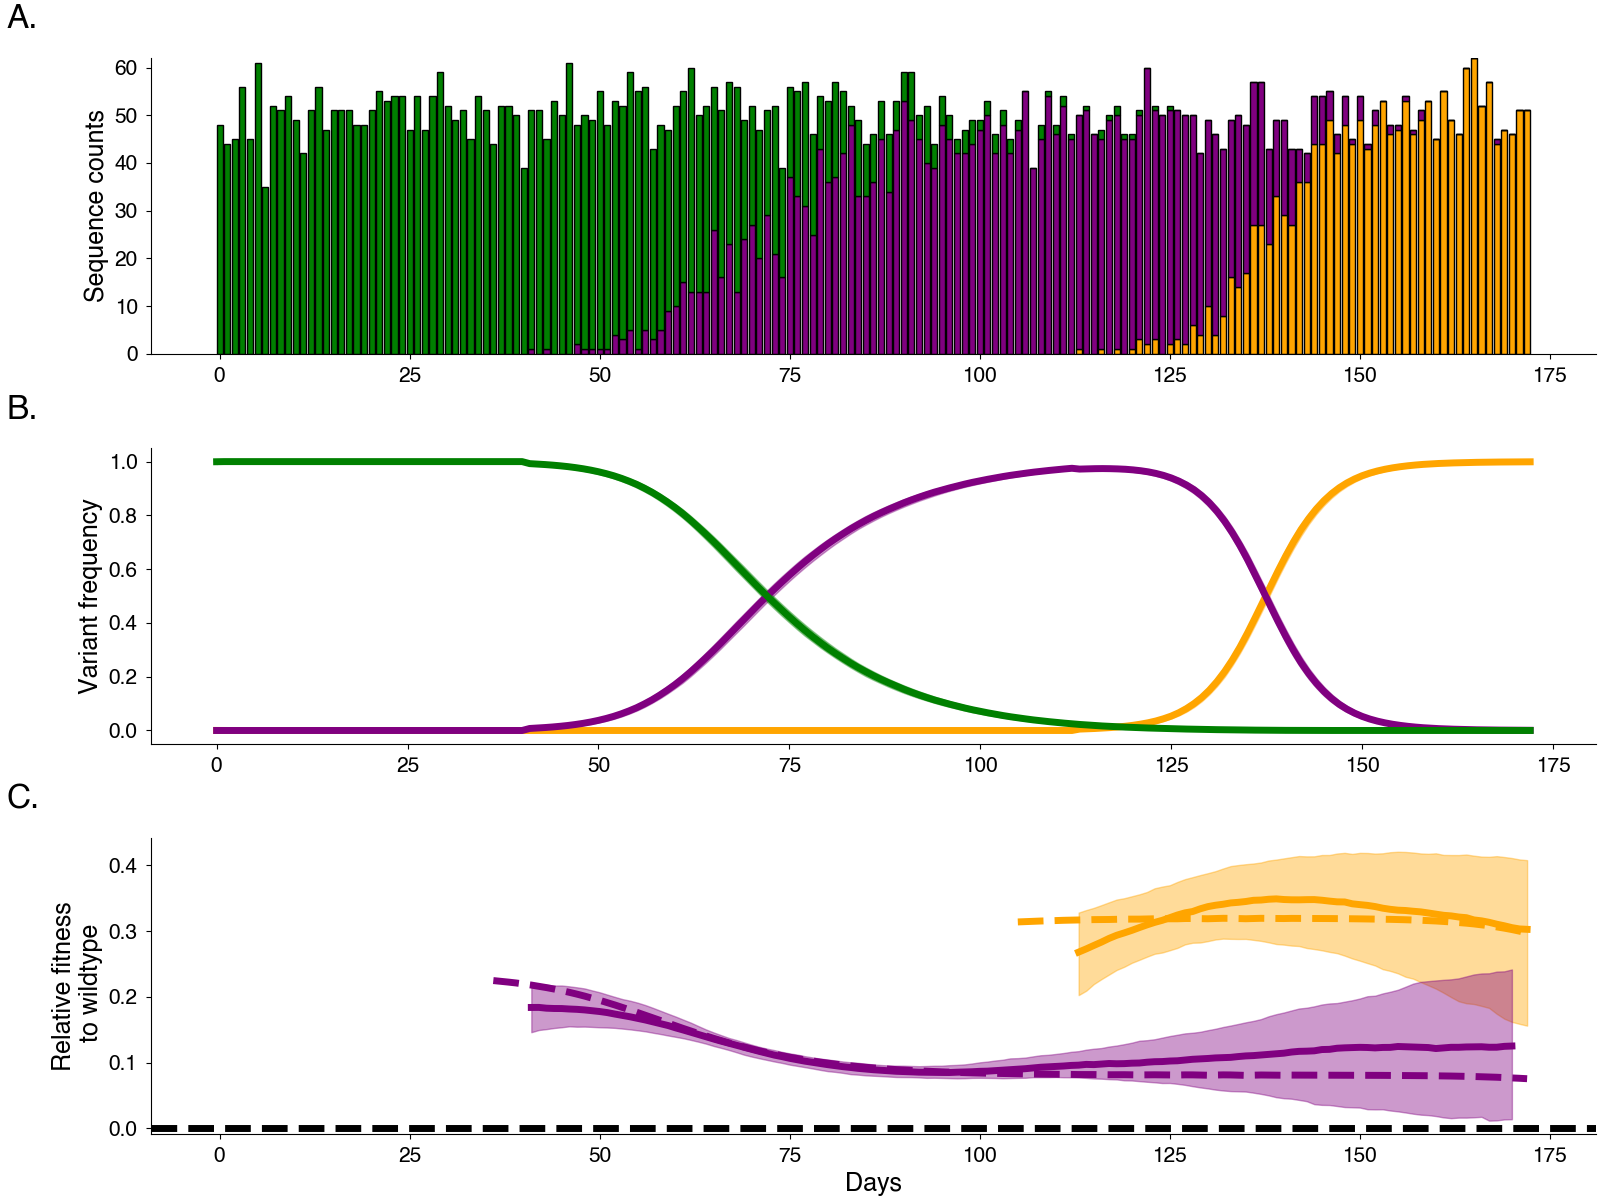
\includegraphics[width=1.0\linewidth]{./supplementary_figures/gp_example.png}
    \caption{
    \textbf{Estimating relative fitness with Gaussian processes.}
      Gaussian processes allow us a non-parametric estimate of the relative fitness for variants through time.
      This figure uses Gaussian processes to model the 3 variant example shown in Fig.~\ref{fig:vis_mechanisms}.
      A. Synthetic sequence counts generated using a multinomial distribution with frequencies from Fig.~\ref{fig:vis_mechanisms}C.
      B. Frequencies and posterior frequencies according to Gaussian process model. Intervals show the 80\% credible interval.
      C. Relative fitnesses. Dashed line shows true relative fitnesses from underlying mechanistic model.
    }
    \label{fig:gp_example}
\end{figure}

\begin{figure}[h]
    \centering
    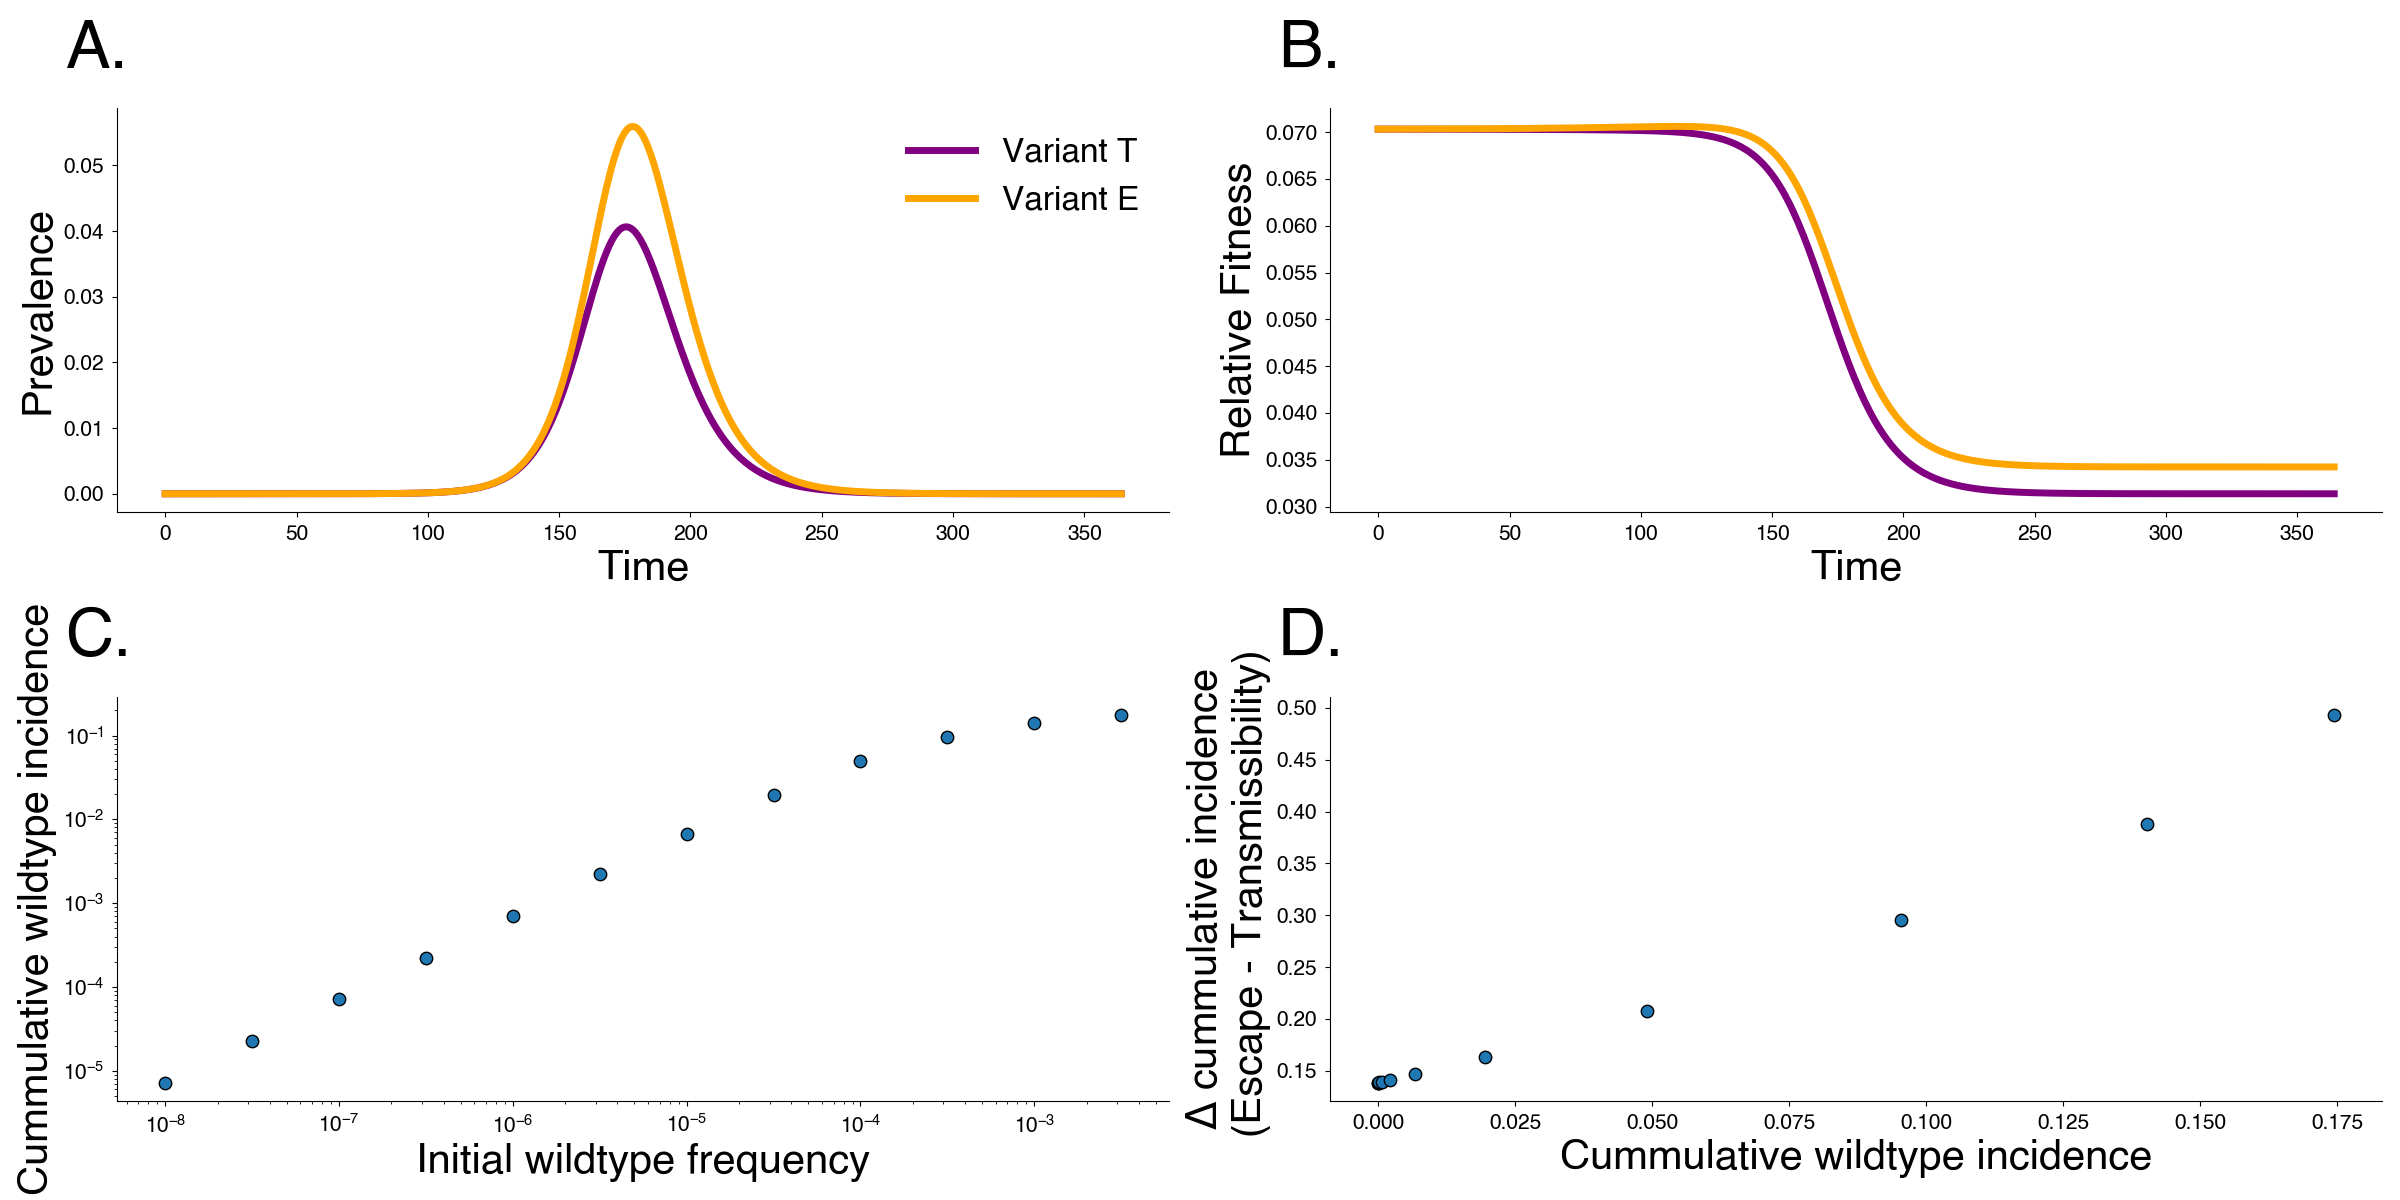
\includegraphics[width=1.0\linewidth]{./supplementary_figures/short_term_divergence.png}
    \caption{
      \textbf{Differences in fitness mechanisms impact frequency and prevalence in the short-term.}
      Comparing simulations from two independent two-variant systems with either an escape variant E (orange) or a transmissibility variant T (purple).
      We fix the initial relative fitness for the two variants using Equation \ref{eq:critical_immunity} and simulate dynamics for 365 days.
      (A) The prevalence for the variants.
      (B) The relative fitness from the variants.
      (C) The cumulative wildtype incidence as a function of the initial wildtype frequency.
      (D) The difference between the cumulative incidence between the escape variant and the transmissibility variant as a function of wildtype incidence.
    }
    \label{fig:short_term_divergence}
\end{figure}

\begin{figure}[t!]
    \centering
    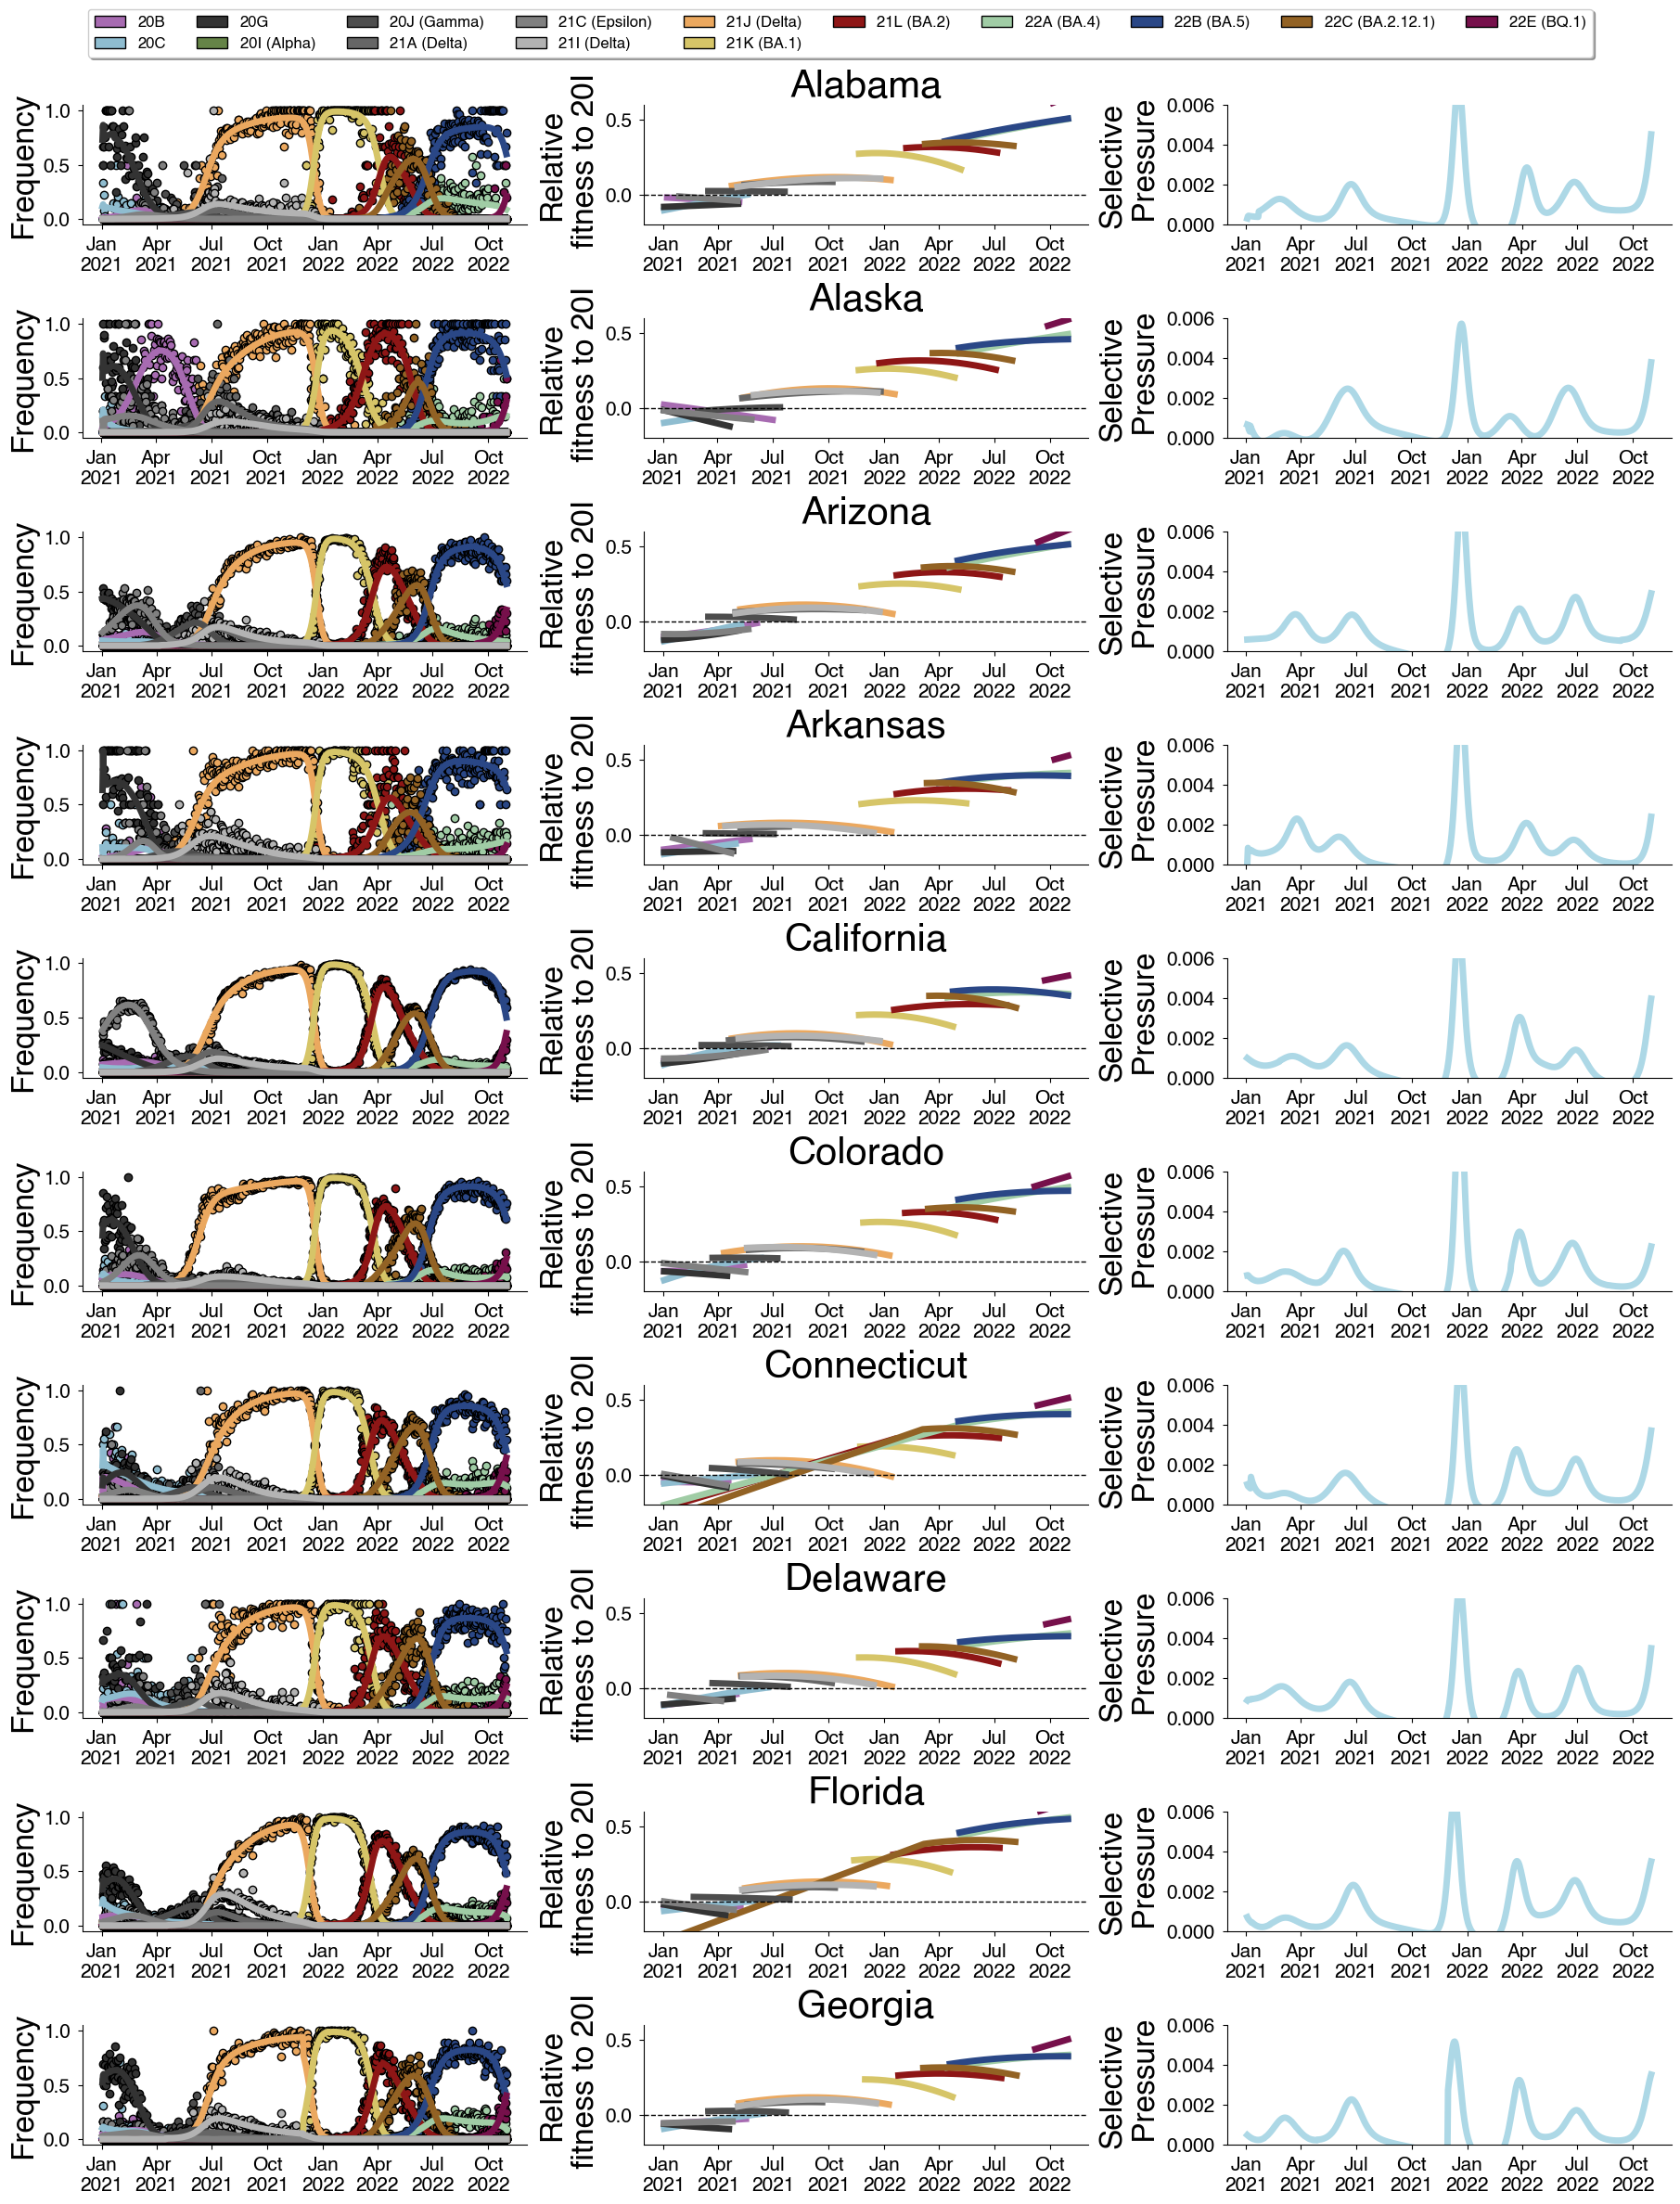
\includegraphics[width=1.0\textwidth=0.01]{./supplementary_figures/selective-pressure-analysis_group_1.png}
    \caption{
      \textbf{Estimated variant frequencies, relative fitnesses, and selective pressure. Alabama through Georgia.}
      \tbc{These requests are for all five selection pressure supp figures.}
      \tbc{I believe the legend has been clipped from the top of figure, restore legend and add WHO / Pango parenthicals to each legend entry, e.g.\ `20I (Alpha)'. An appropriate set of labels can be seen here \url{http://github.com/nextstrain/ncov/blob/master/defaults/clade_display_names.yml}}
    }
    \label{fig:selective_pressure_group_1}
\end{figure}

\begin{figure}[t!]
    \centering
    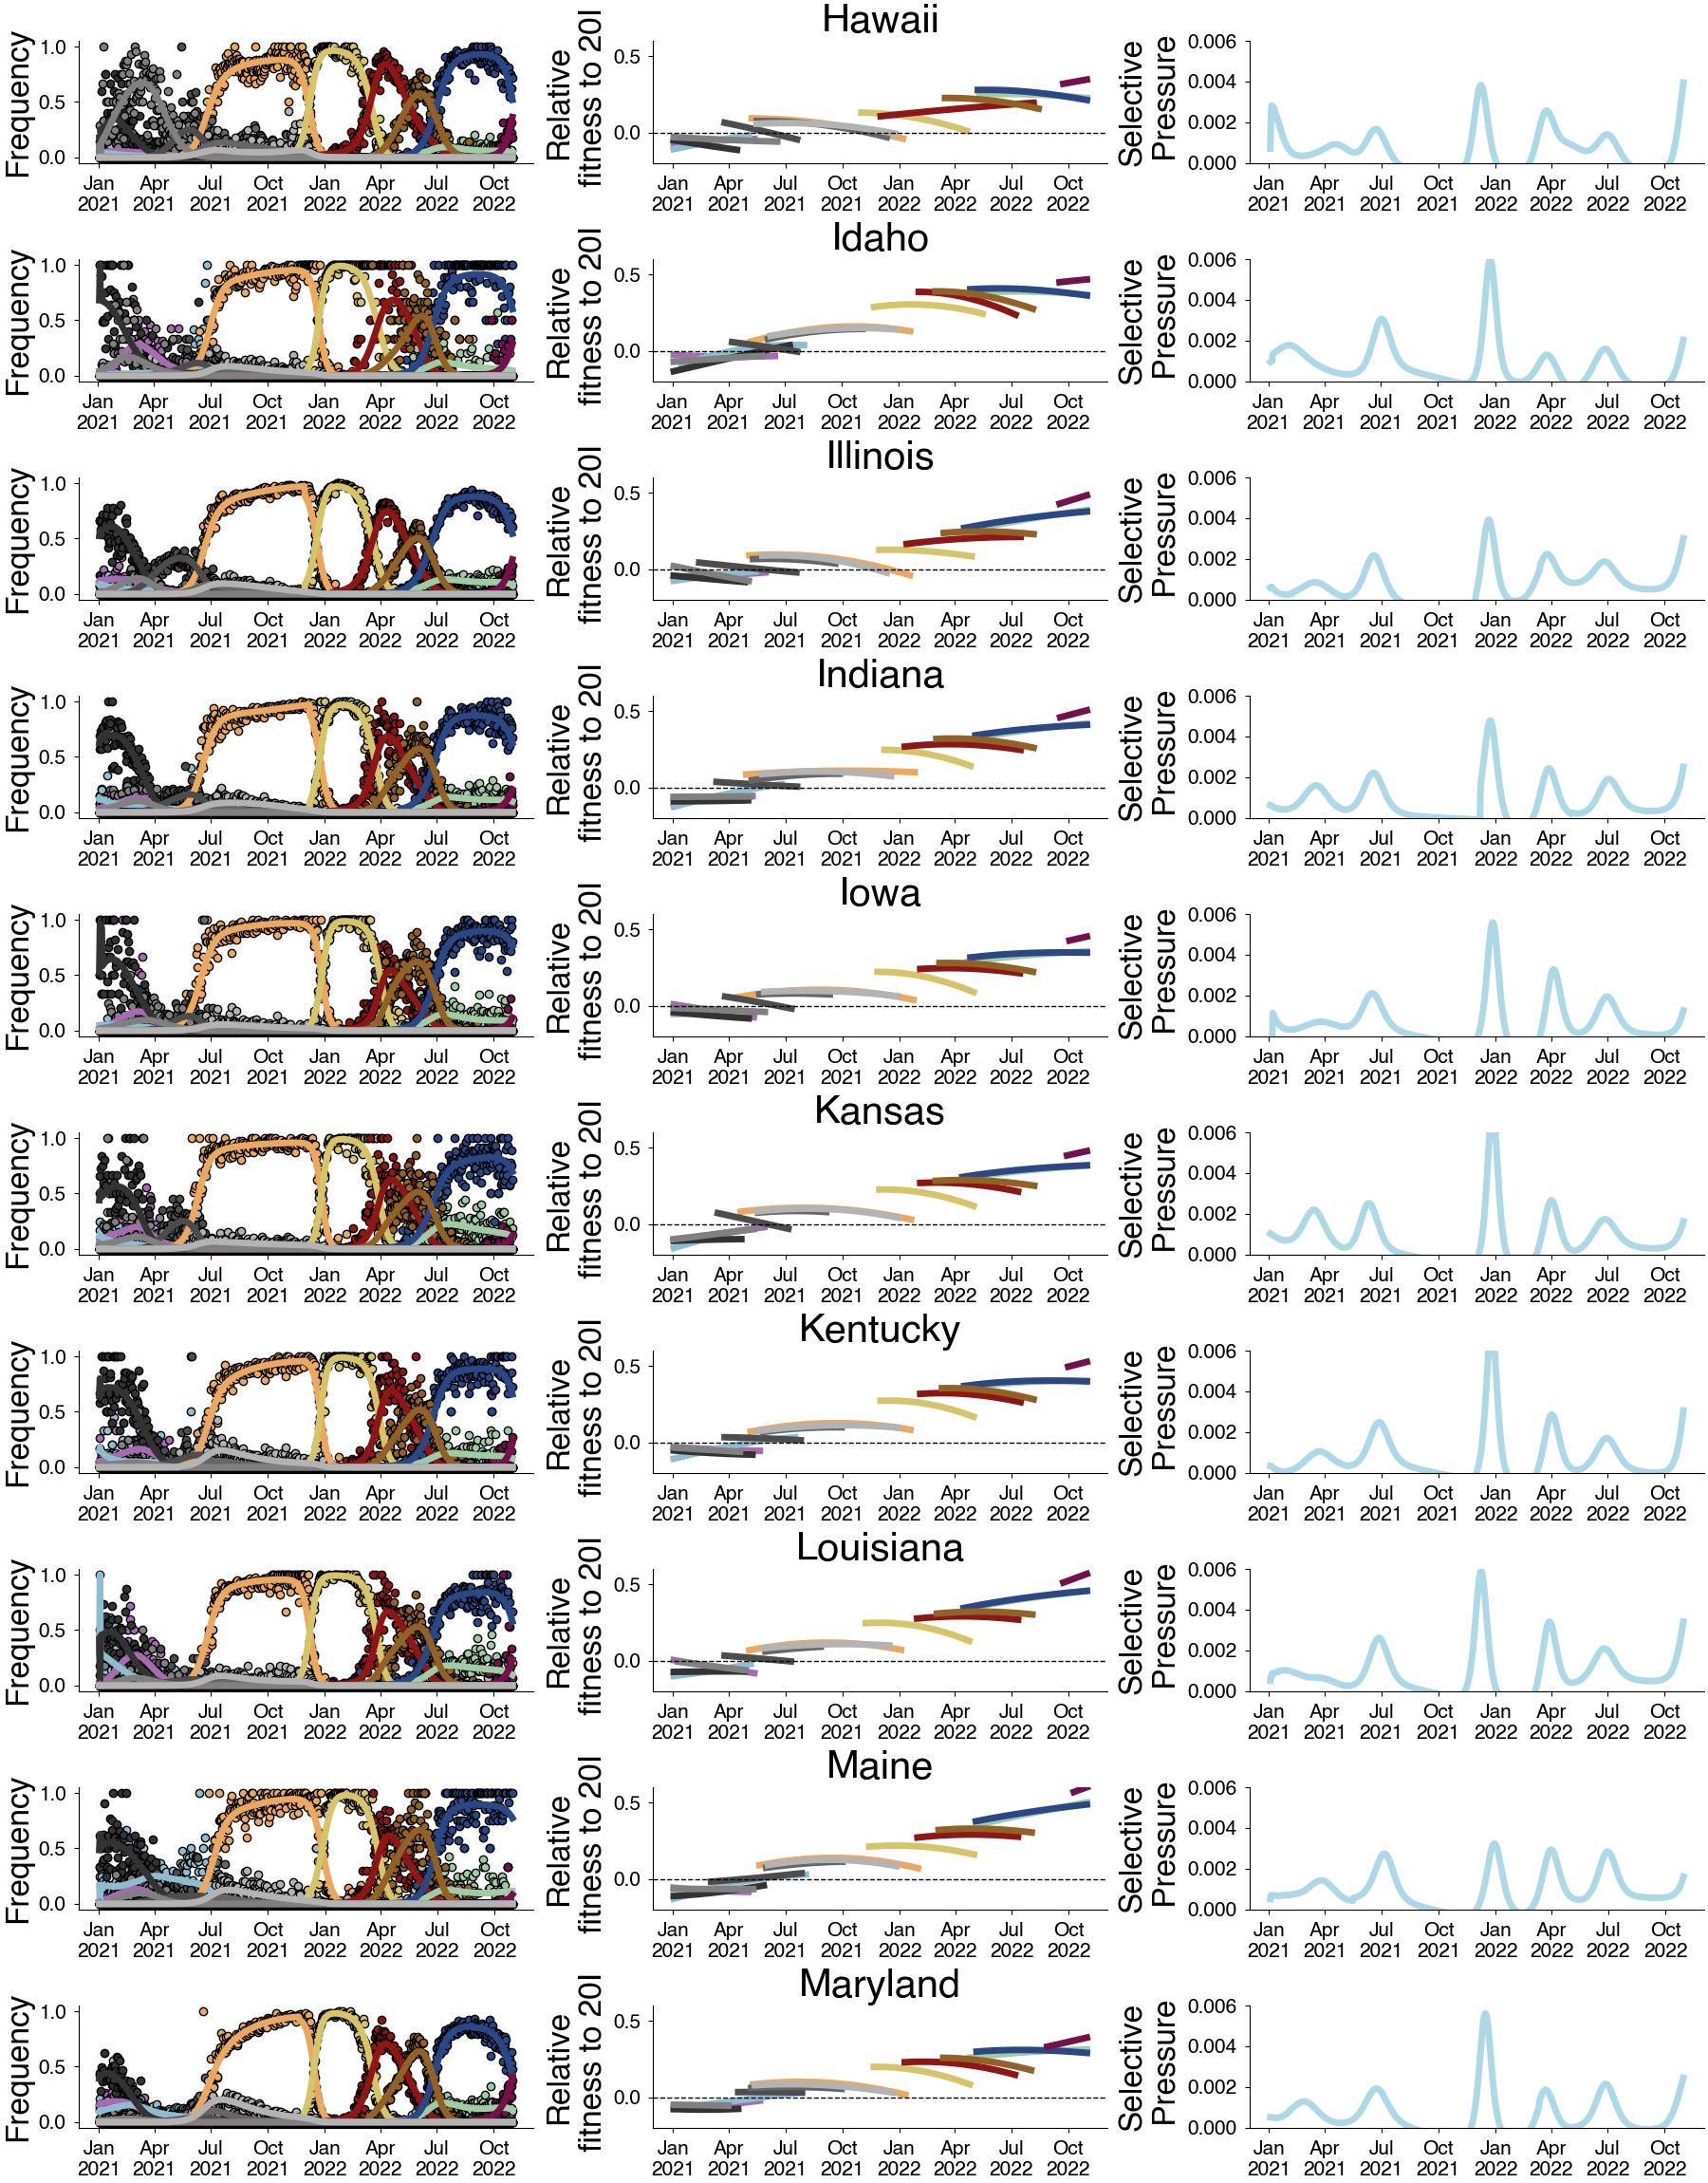
\includegraphics[width=1.0\textwidth=0.01]{./supplementary_figures/selective-pressure-analysis_group_2.png}
    \caption{
        \textbf{Estimated variant frequencies, relative fitnesses, and selective pressure. Hawaii to Maryland.}
    }
    \label{fig:selective_pressure_group_2}
\end{figure}

\begin{figure}[t!]
    \centering
    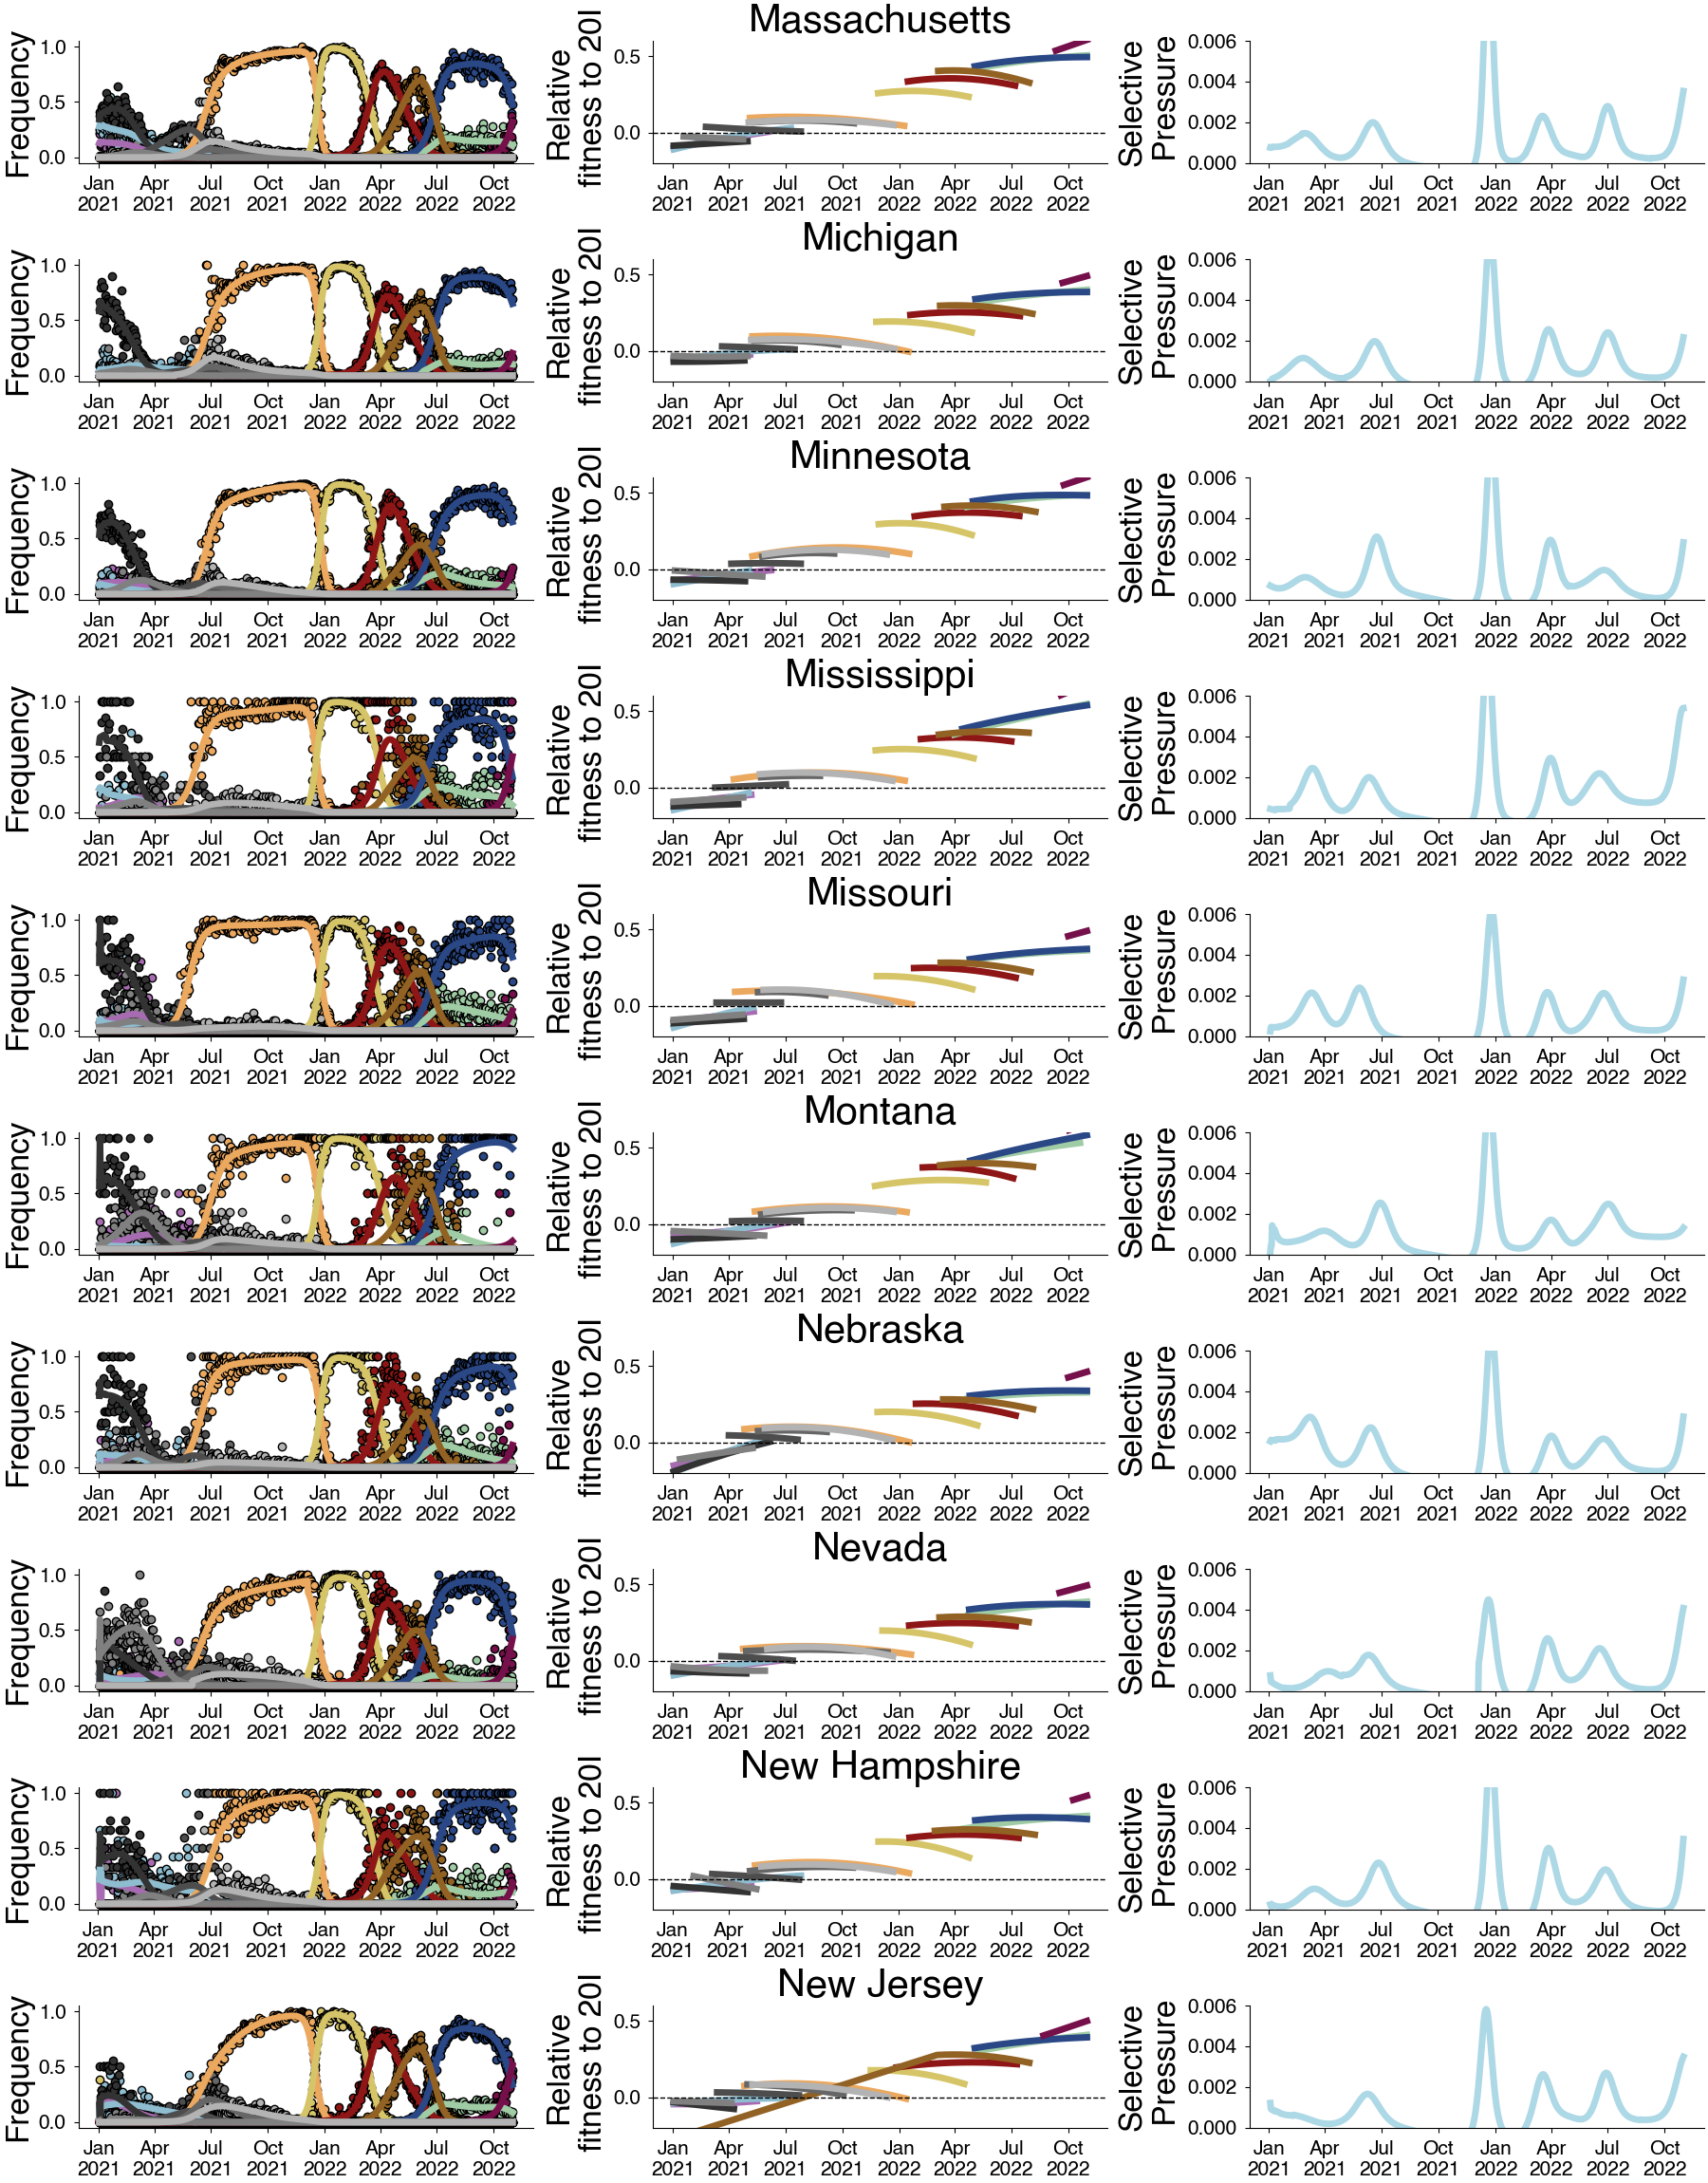
\includegraphics[width=1.0\textwidth=0.01]{./supplementary_figures/selective-pressure-analysis_group_3.png}
    \caption{
      \textbf{Estimated variant frequencies, relative fitnesses, and selective pressure. Massachusetts to New Jersey.}
    }
    \label{fig:selective_pressure_group_3}
\end{figure}

\begin{figure}[t!]
    \centering
    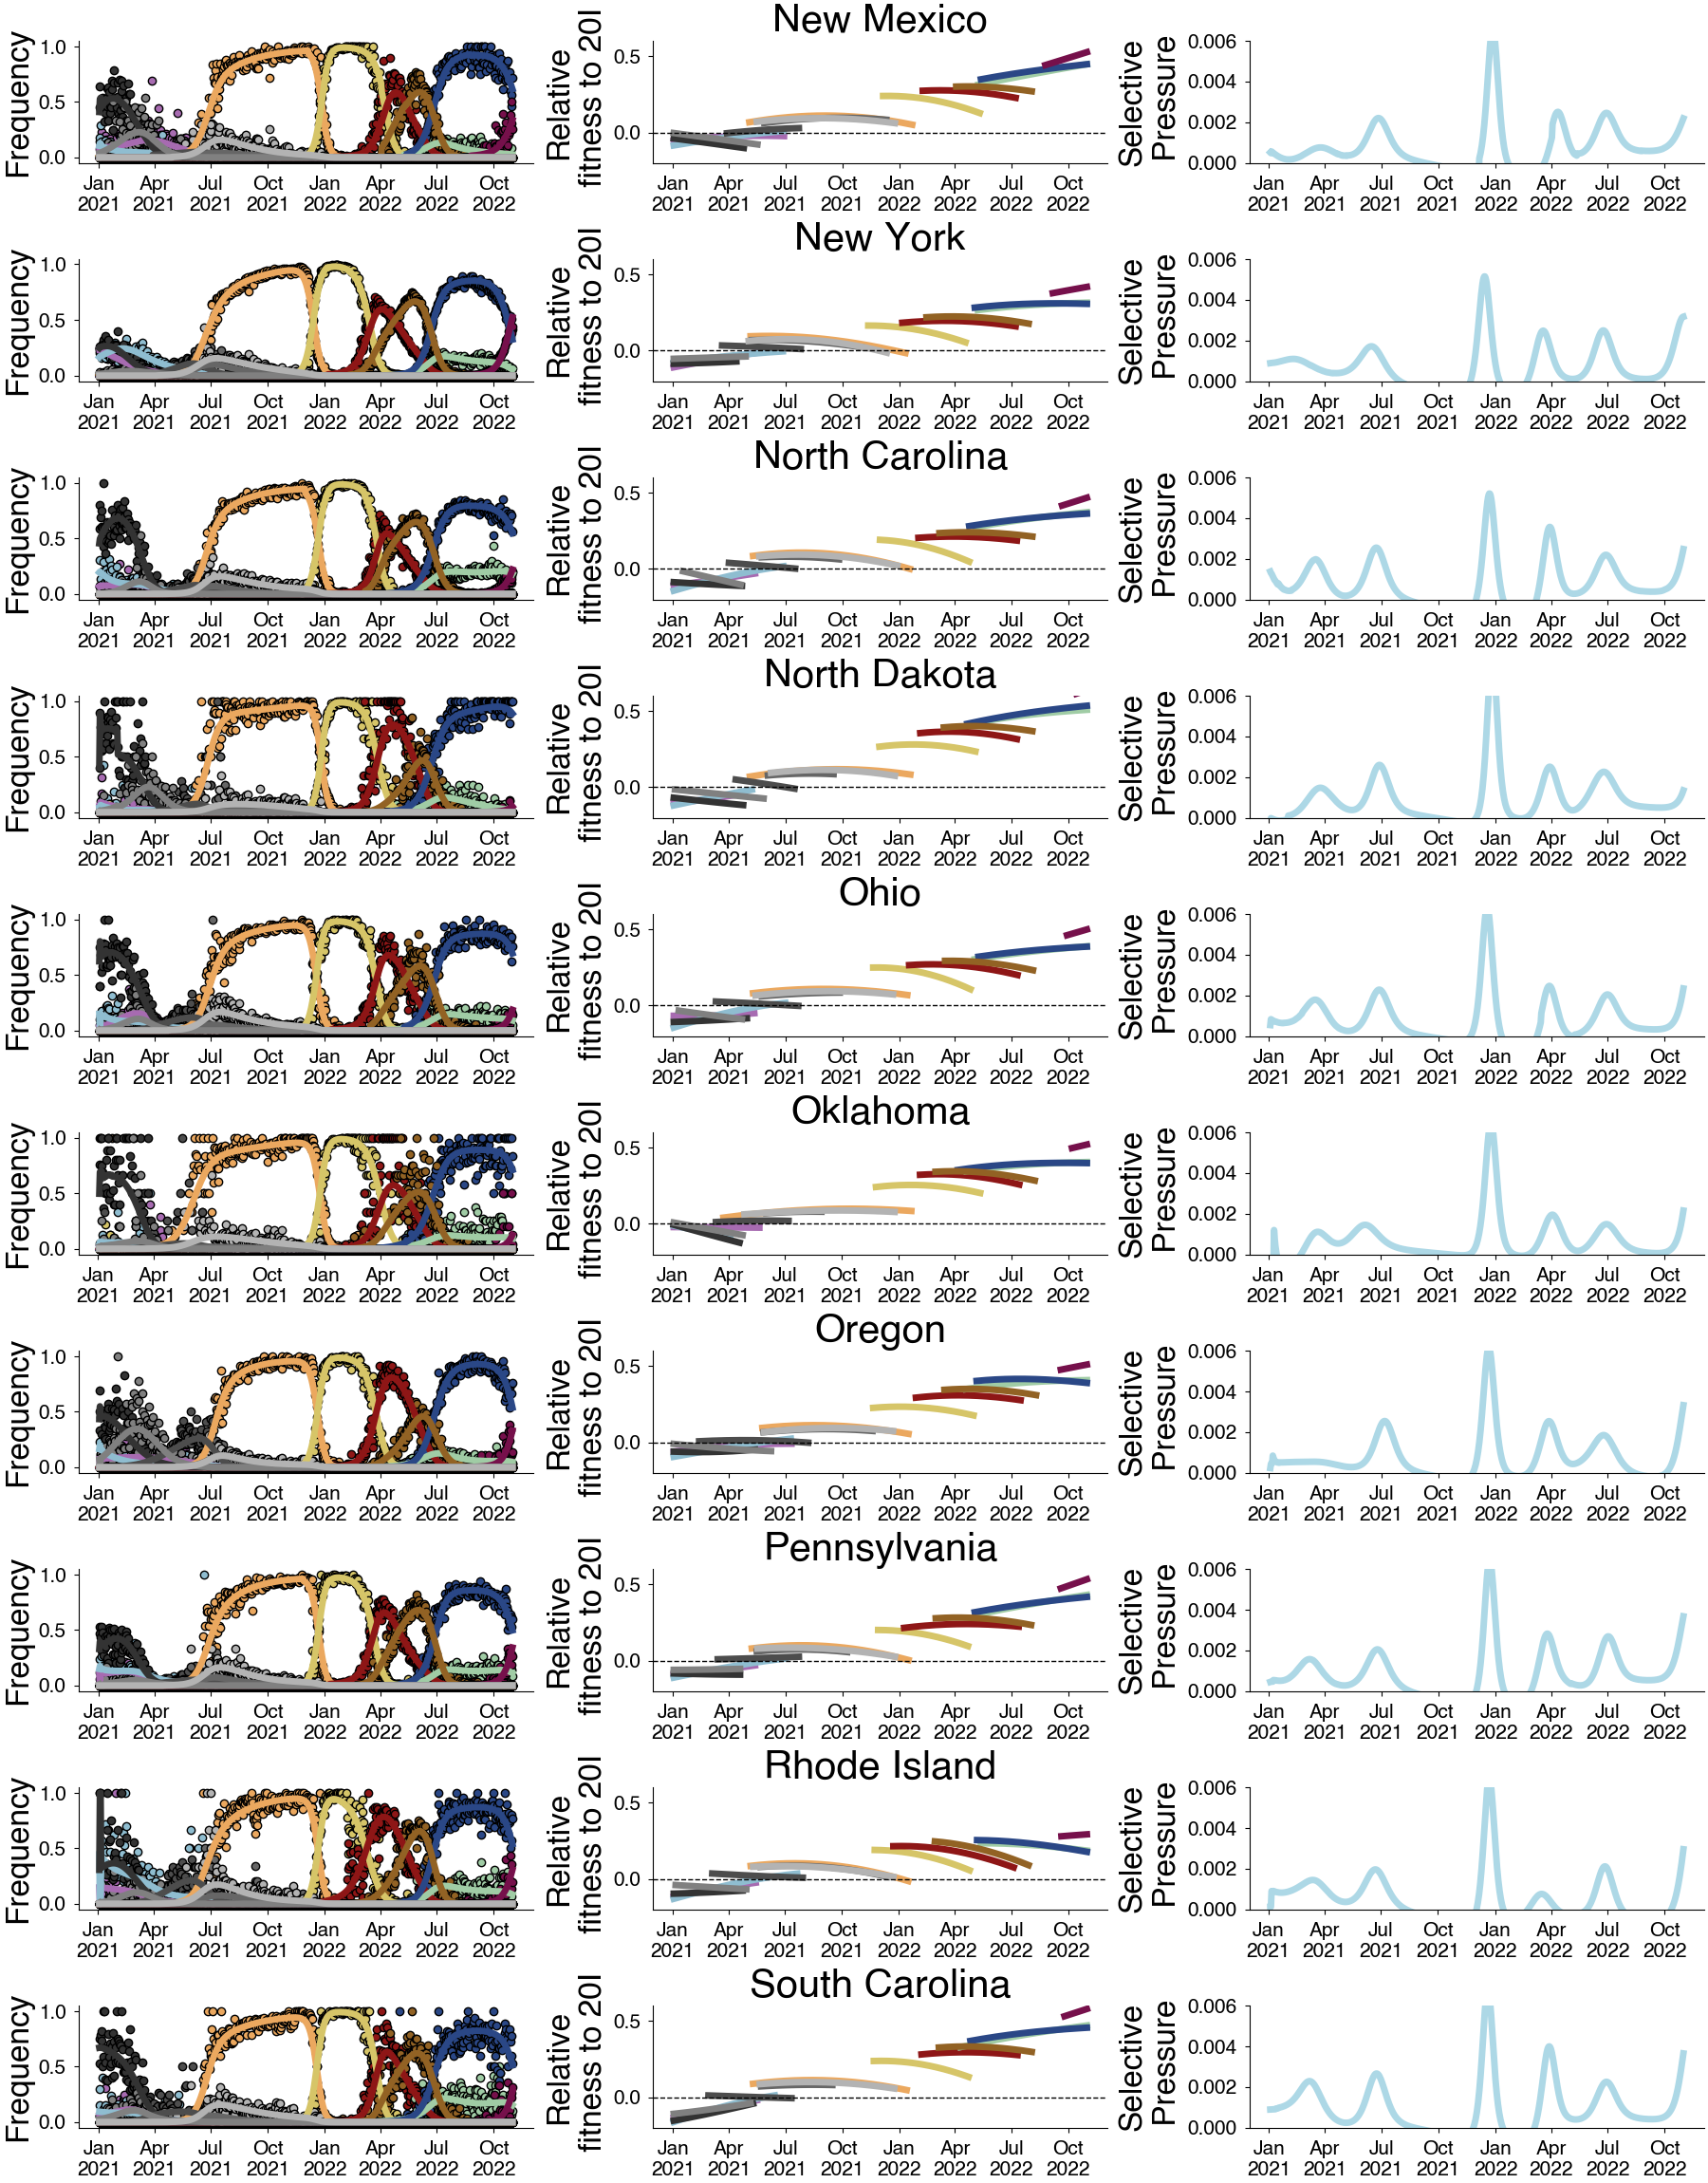
\includegraphics[width=1.0\textwidth=0.01]{./supplementary_figures/selective-pressure-analysis_group_4.png}
    \caption{
      \textbf{Estimated variant frequencies, relative fitnesses, and selective pressure. New Mexico to South Carolina.}
    }
    \label{fig:selective_pressure_group_4}
\end{figure}

\begin{figure}[t!]
    \centering
    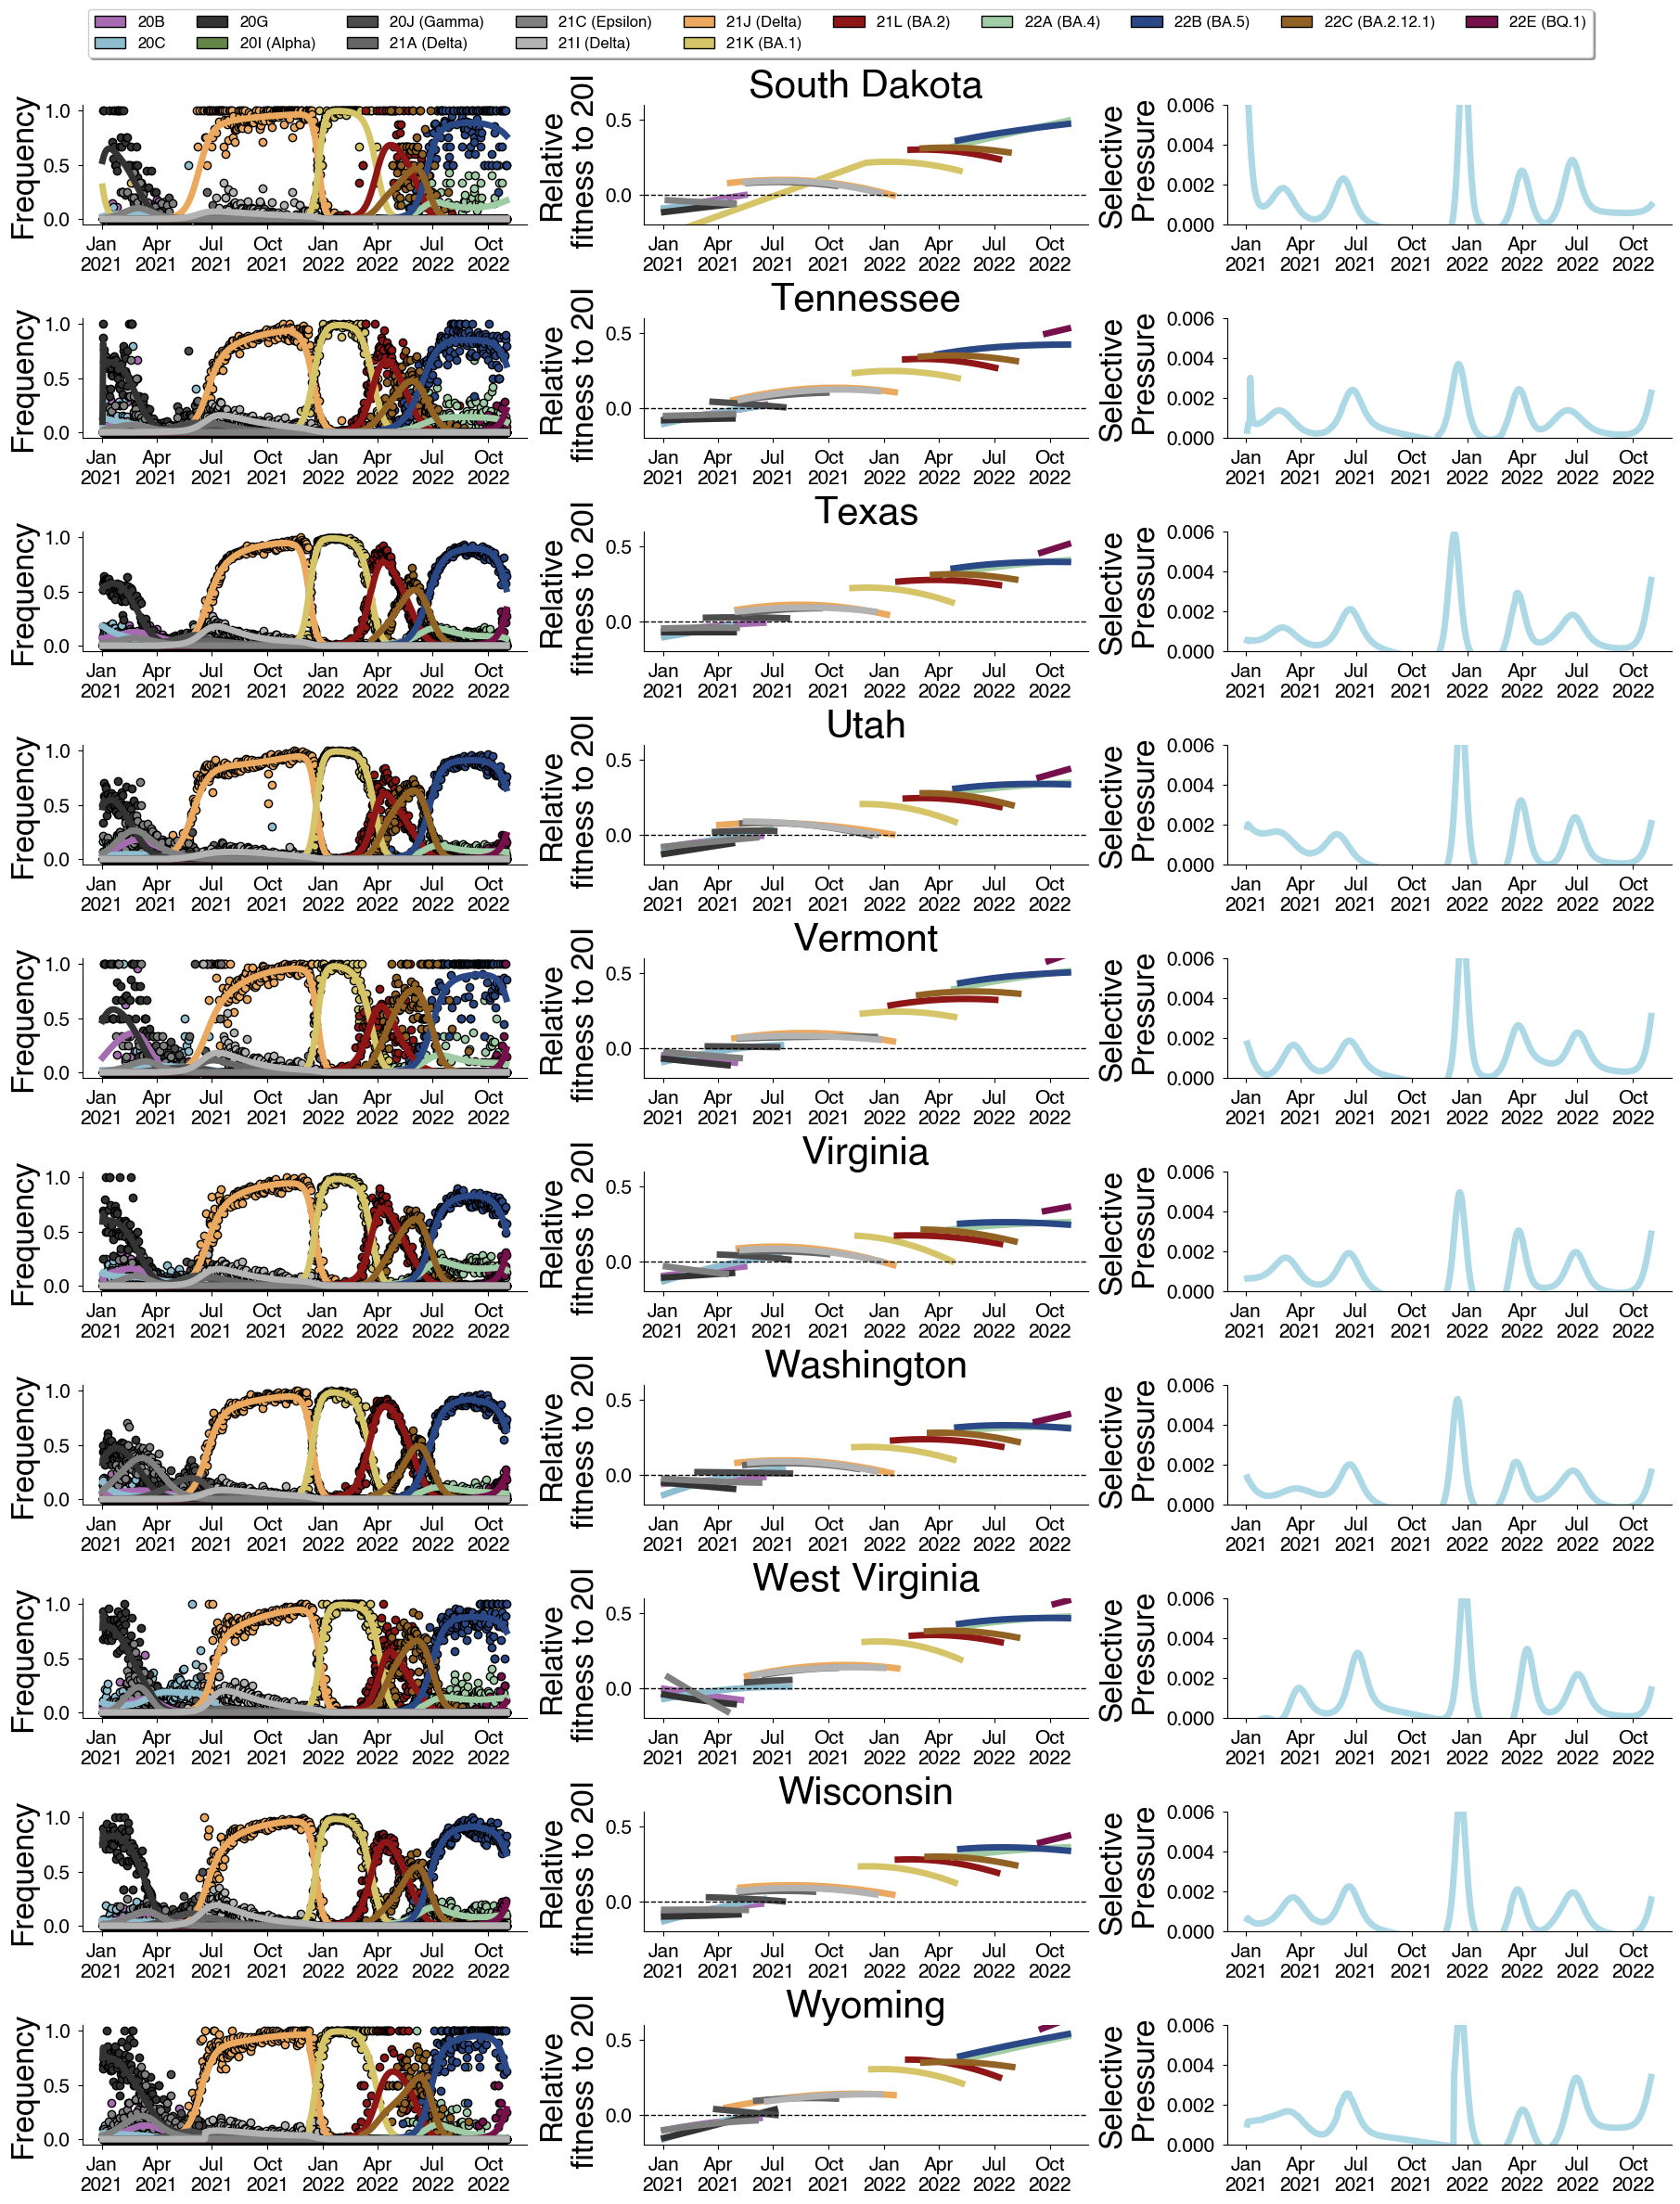
\includegraphics[width=1.0\textwidth=0.01]{./supplementary_figures/selective-pressure-analysis_group_5.png}
    \caption{
      \textbf{Estimated variant frequencies, relative fitnesses, and selective pressure. South Dakota to Wyoming.}
    }
    \label{fig:selective_pressure_group_5}
\end{figure}

\begin{figure}[t!]
    \centering
    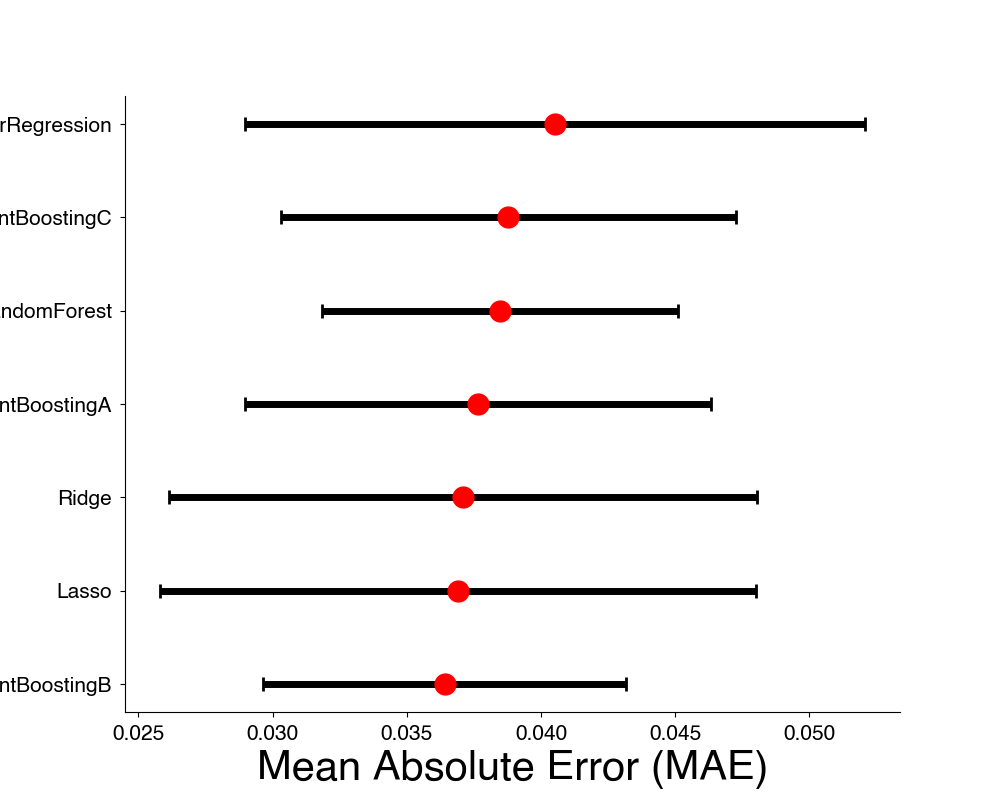
\includegraphics[width=1.0\textwidth=0.01]{./supplementary_figures/growth-rate-prediction-model-comparison.png}
    \caption{
      \textbf{Cross-validation error by model}
      We compare the errors between models fit on 5 time series cross-validation splits.
    }
    \label{fig:growth_rate_predictions_model_comparison}
\end{figure}

\begin{figure}[t!]
    \centering
    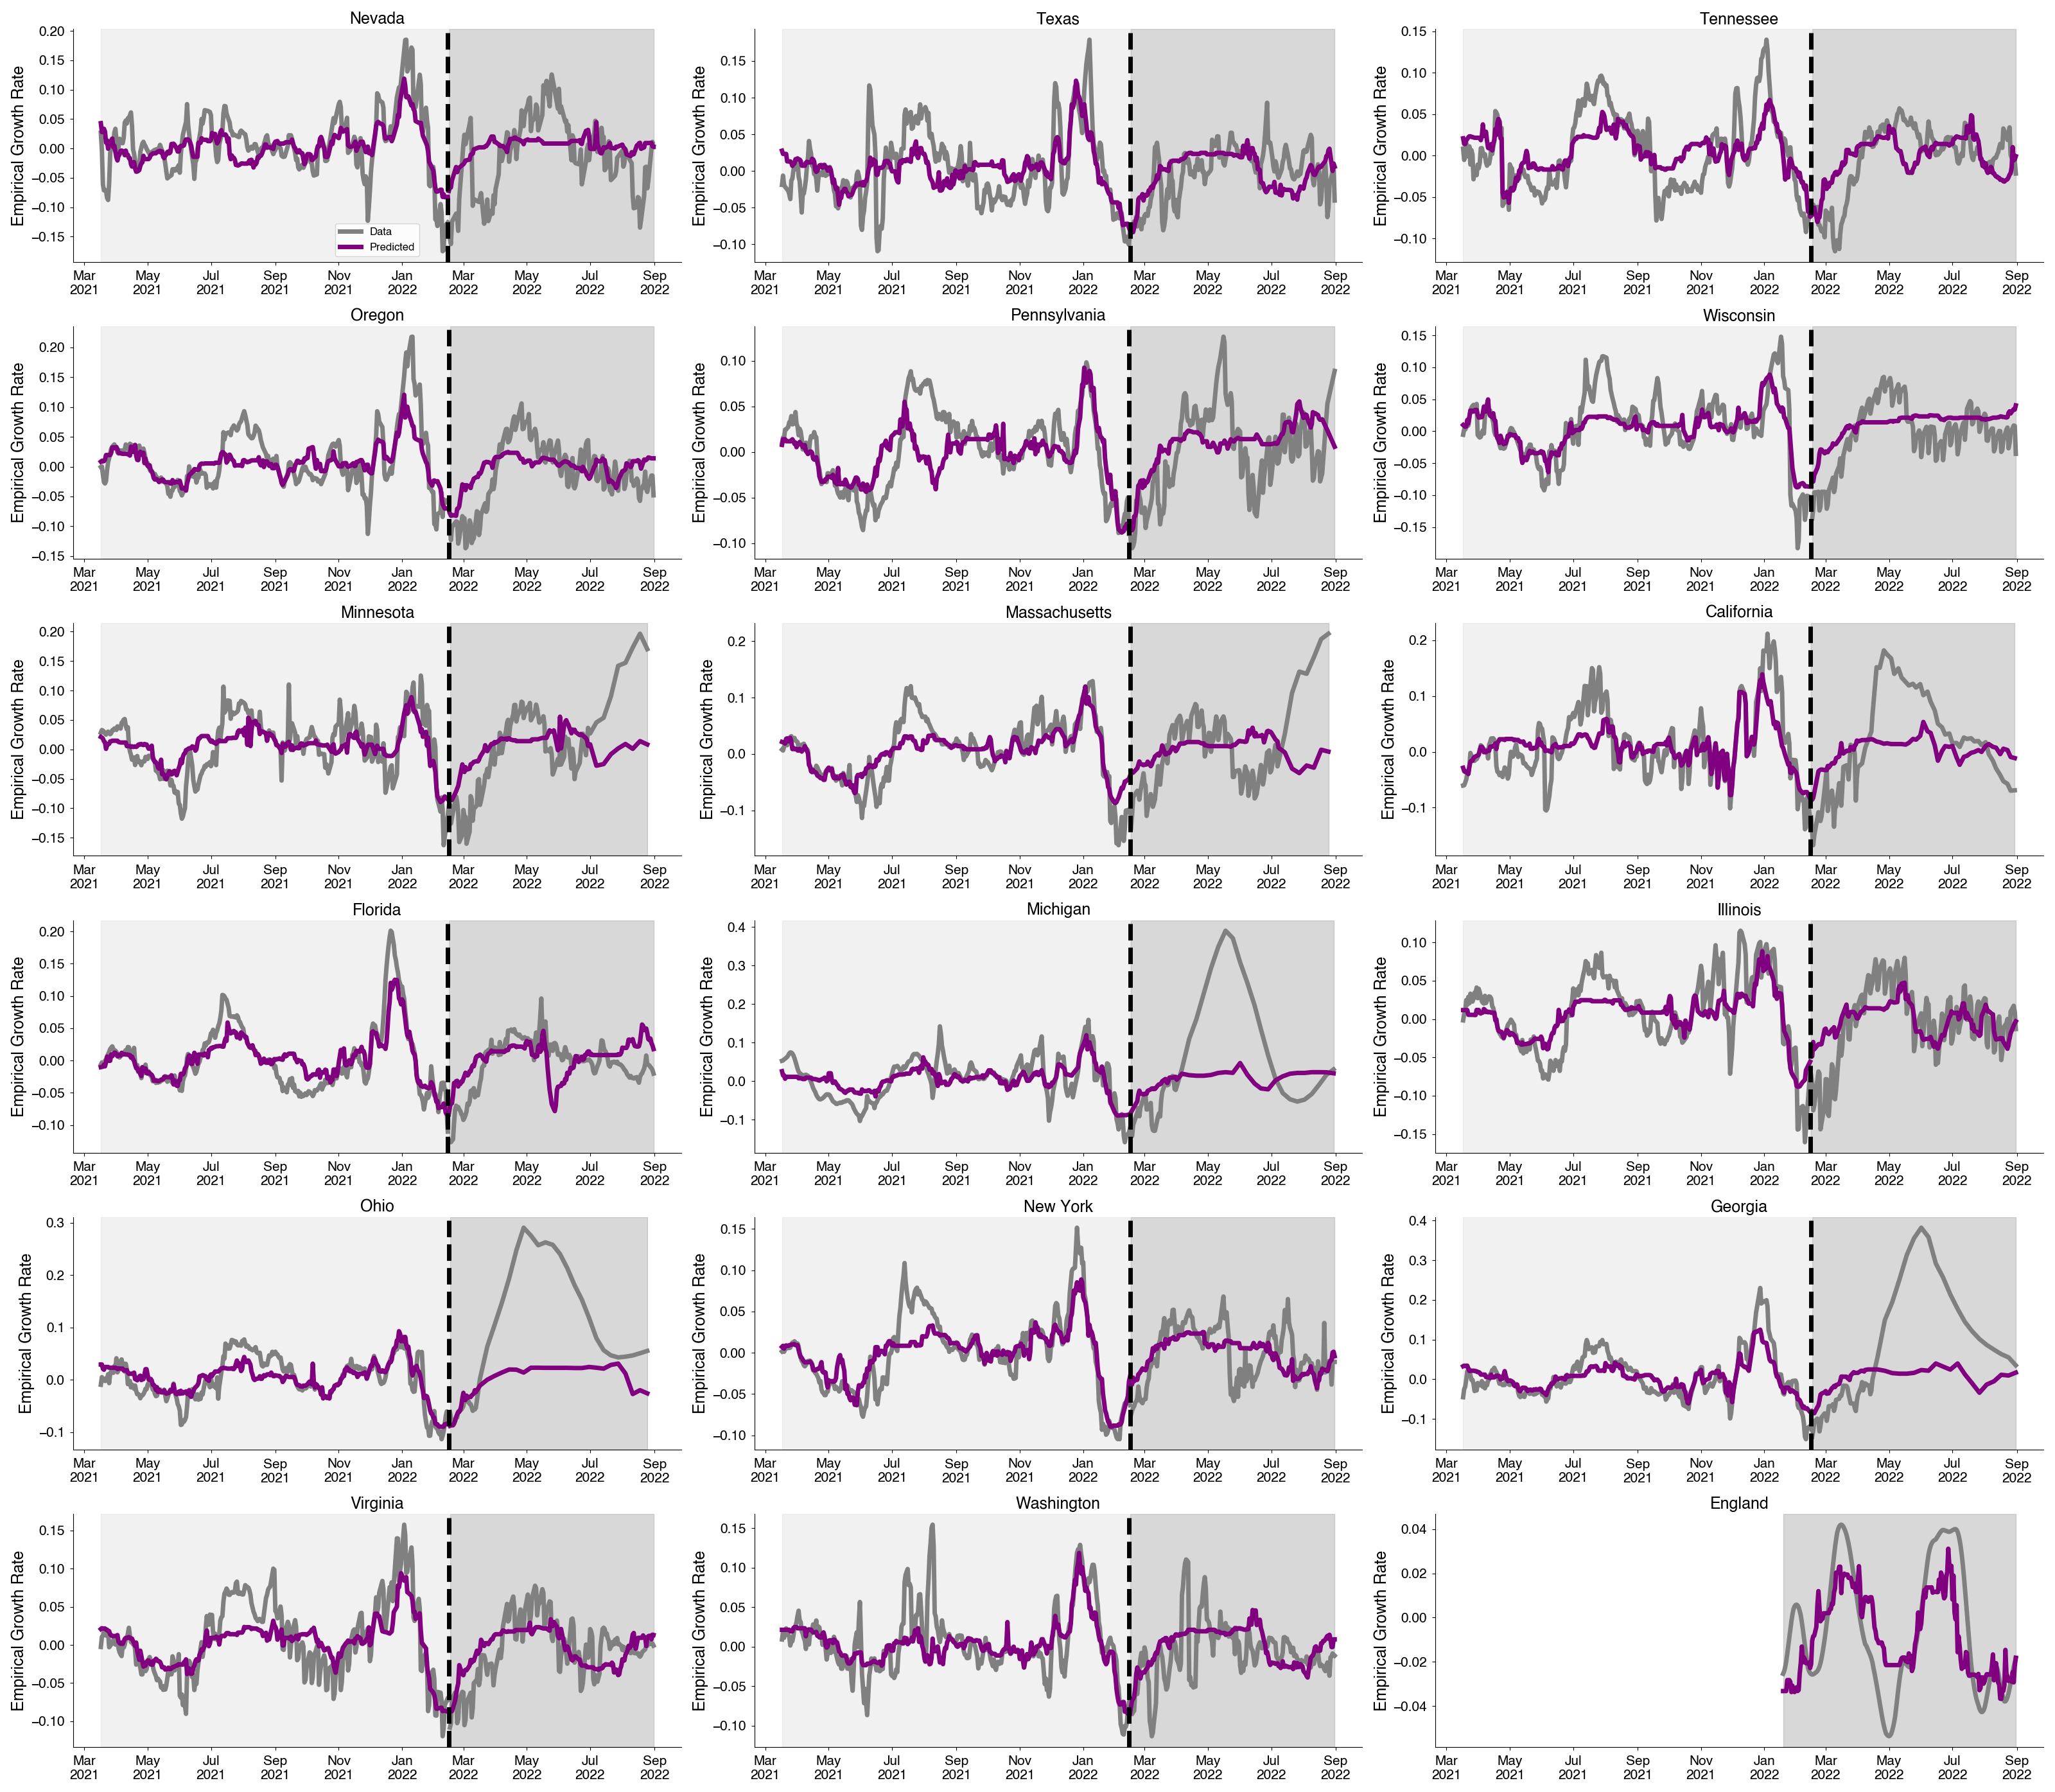
\includegraphics[width=1.0\textwidth=0.01]{./supplementary_figures/empirical_growth_rate_predictions_all.png}
    \caption{
      \textbf{Predictions for empirical growth rate using selective pressure for all locations.}
      % \tbc{Include another supplemental figure showing variant frequencies and selective pressures across all locations. It's important to `show the data' as much as possible.}
    }
    \label{fig:empirical_growth_rate_predictions_all}
\end{figure}


\begin{figure}[t!]
    \centering
    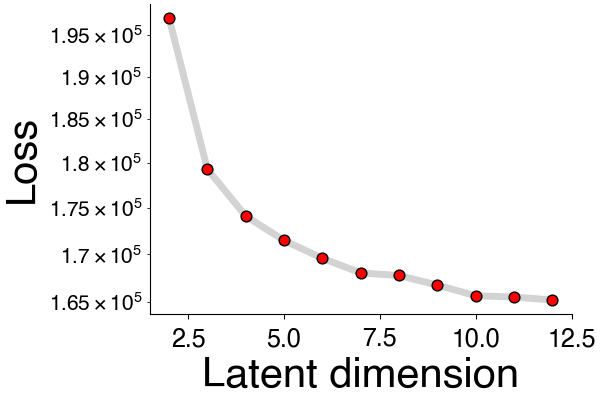
\includegraphics[width=1.0\textwidth=0.01]{./supplementary_figures/loss_by_latent_dimension.png}
    \caption{
      \textbf{Maximum a posteriori loss for latent factor model by number of latent immune dimensions.}
    }
    \label{fig:latent_factor_dimension}
\end{figure}

\begin{figure}[t!]
    \centering
    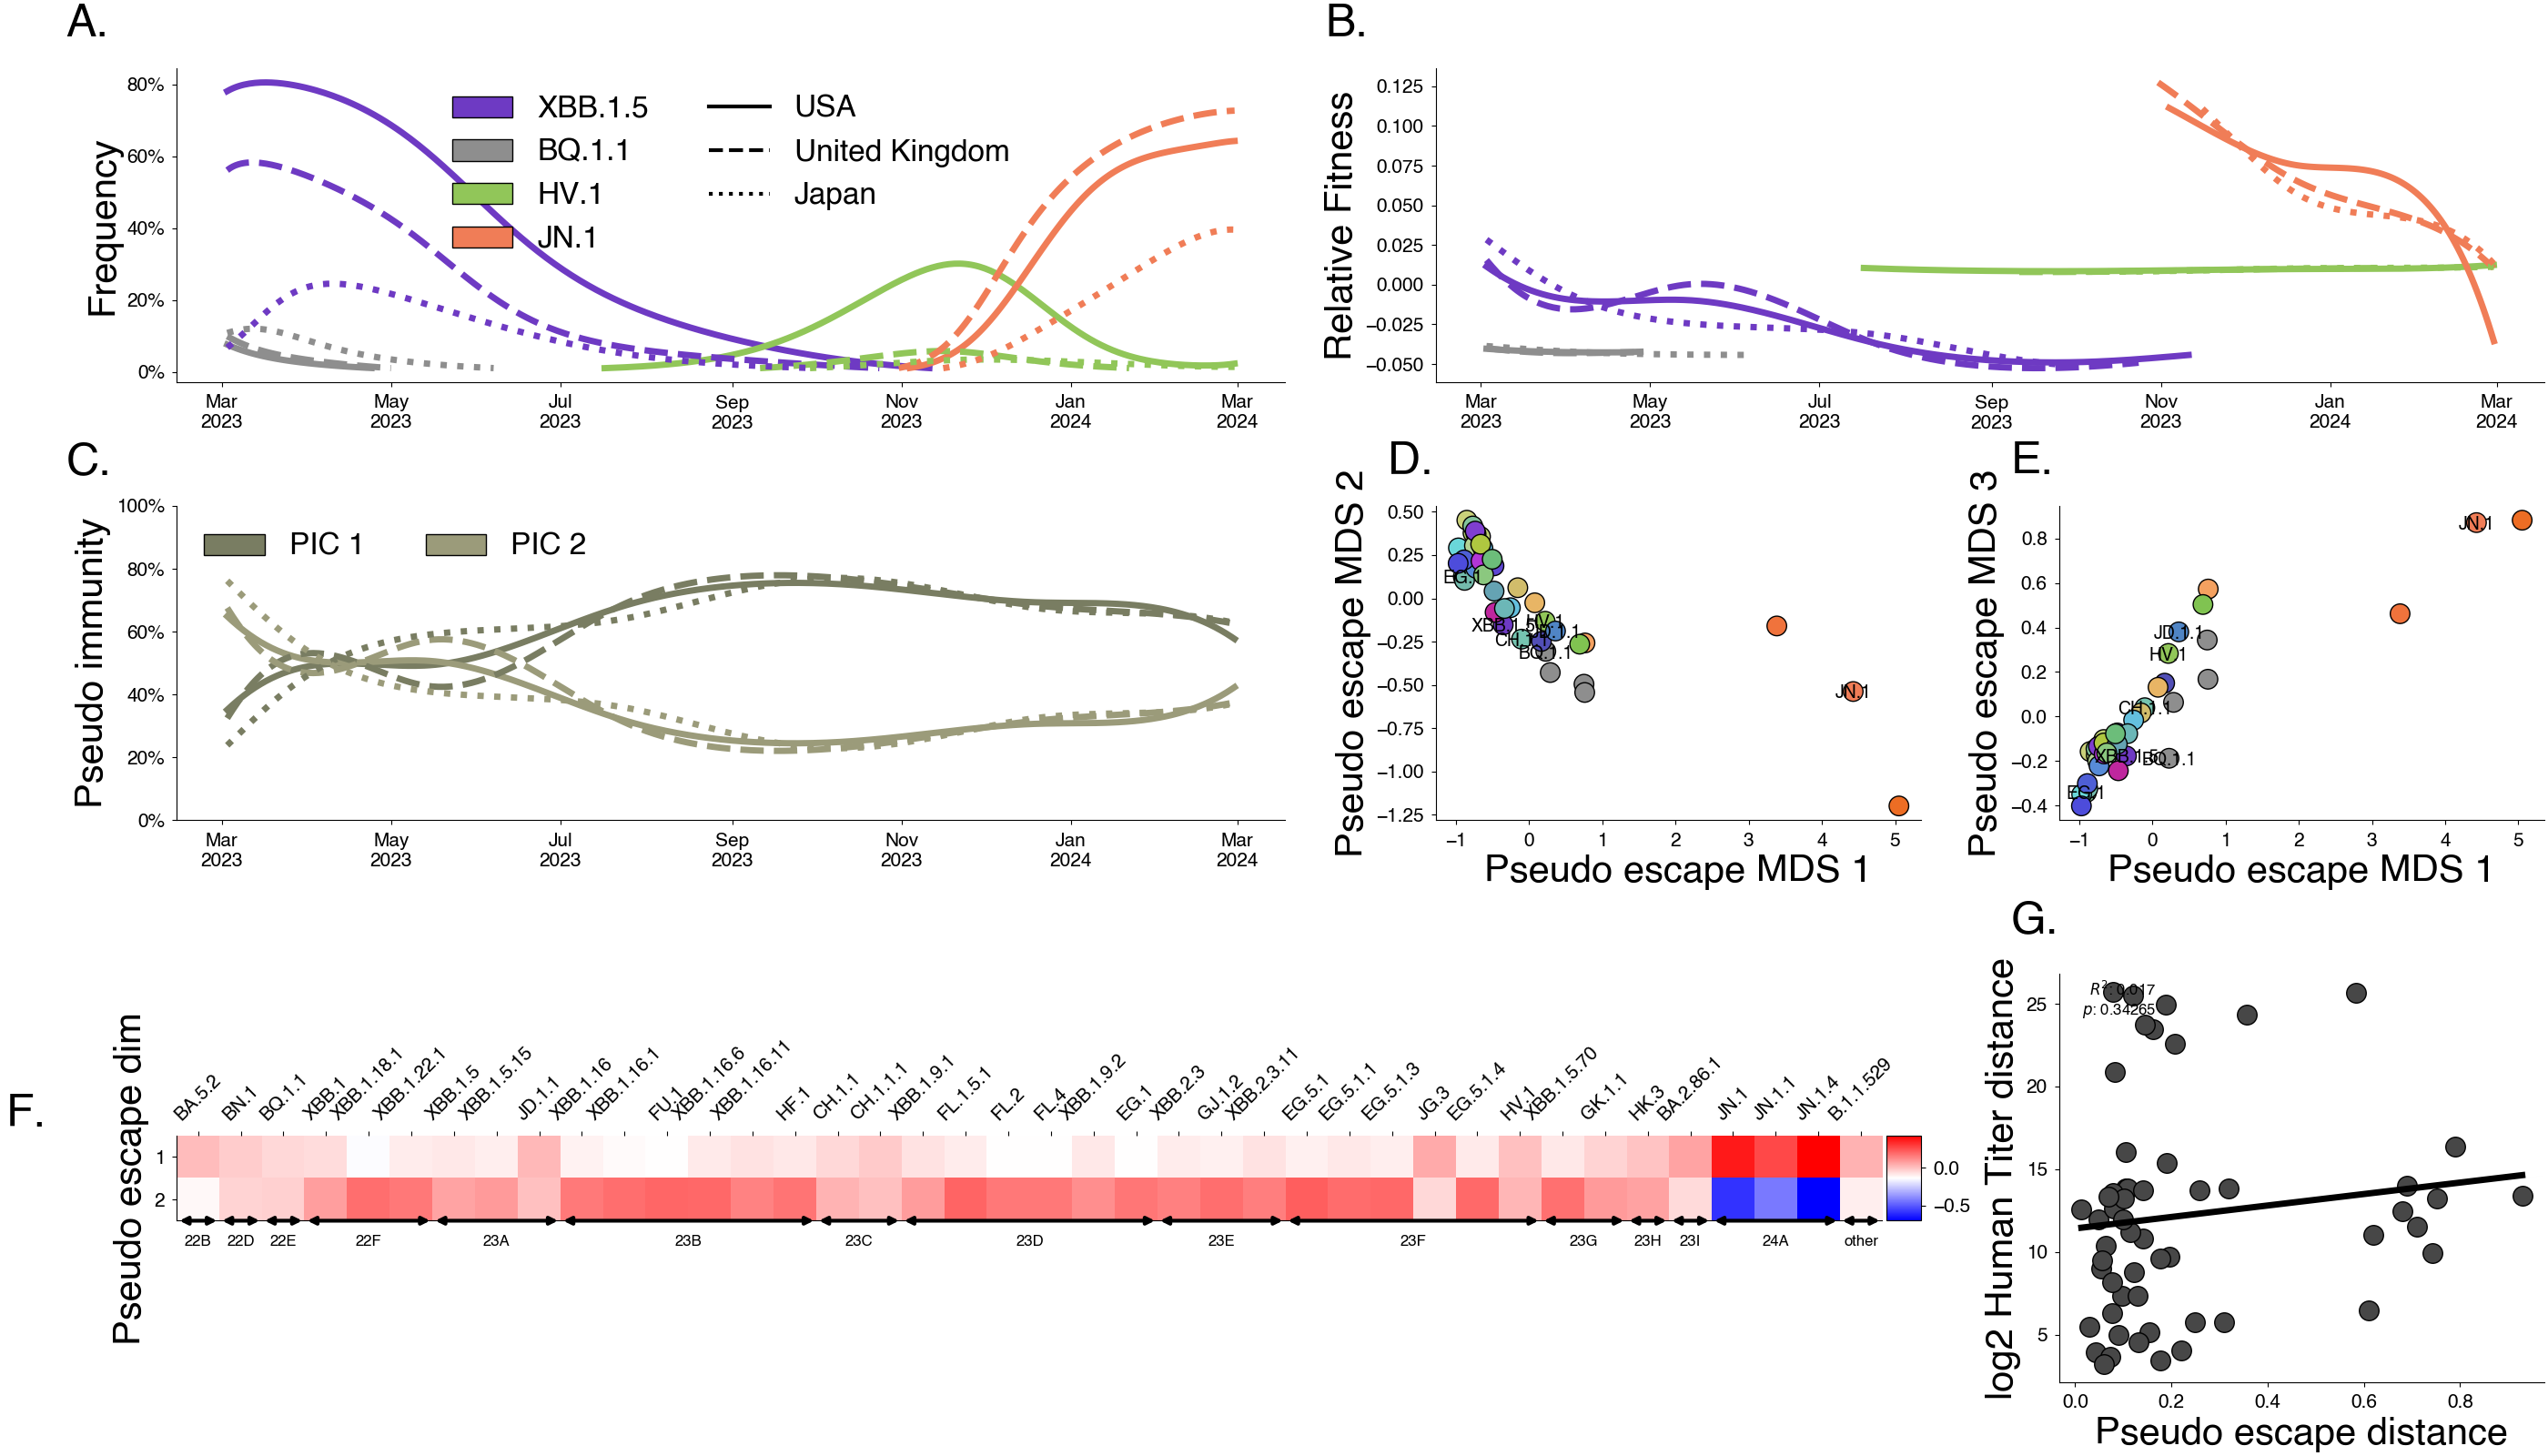
\includegraphics[width=1.0\textwidth=0.01]{./supplementary_figures/latent_immune_2_dims.png}
    \caption{
      \textbf{Latent factor model. $D=2$}
    }
    \label{fig:latent_factor_2}
\end{figure}

\begin{figure}[t!]
    \centering
    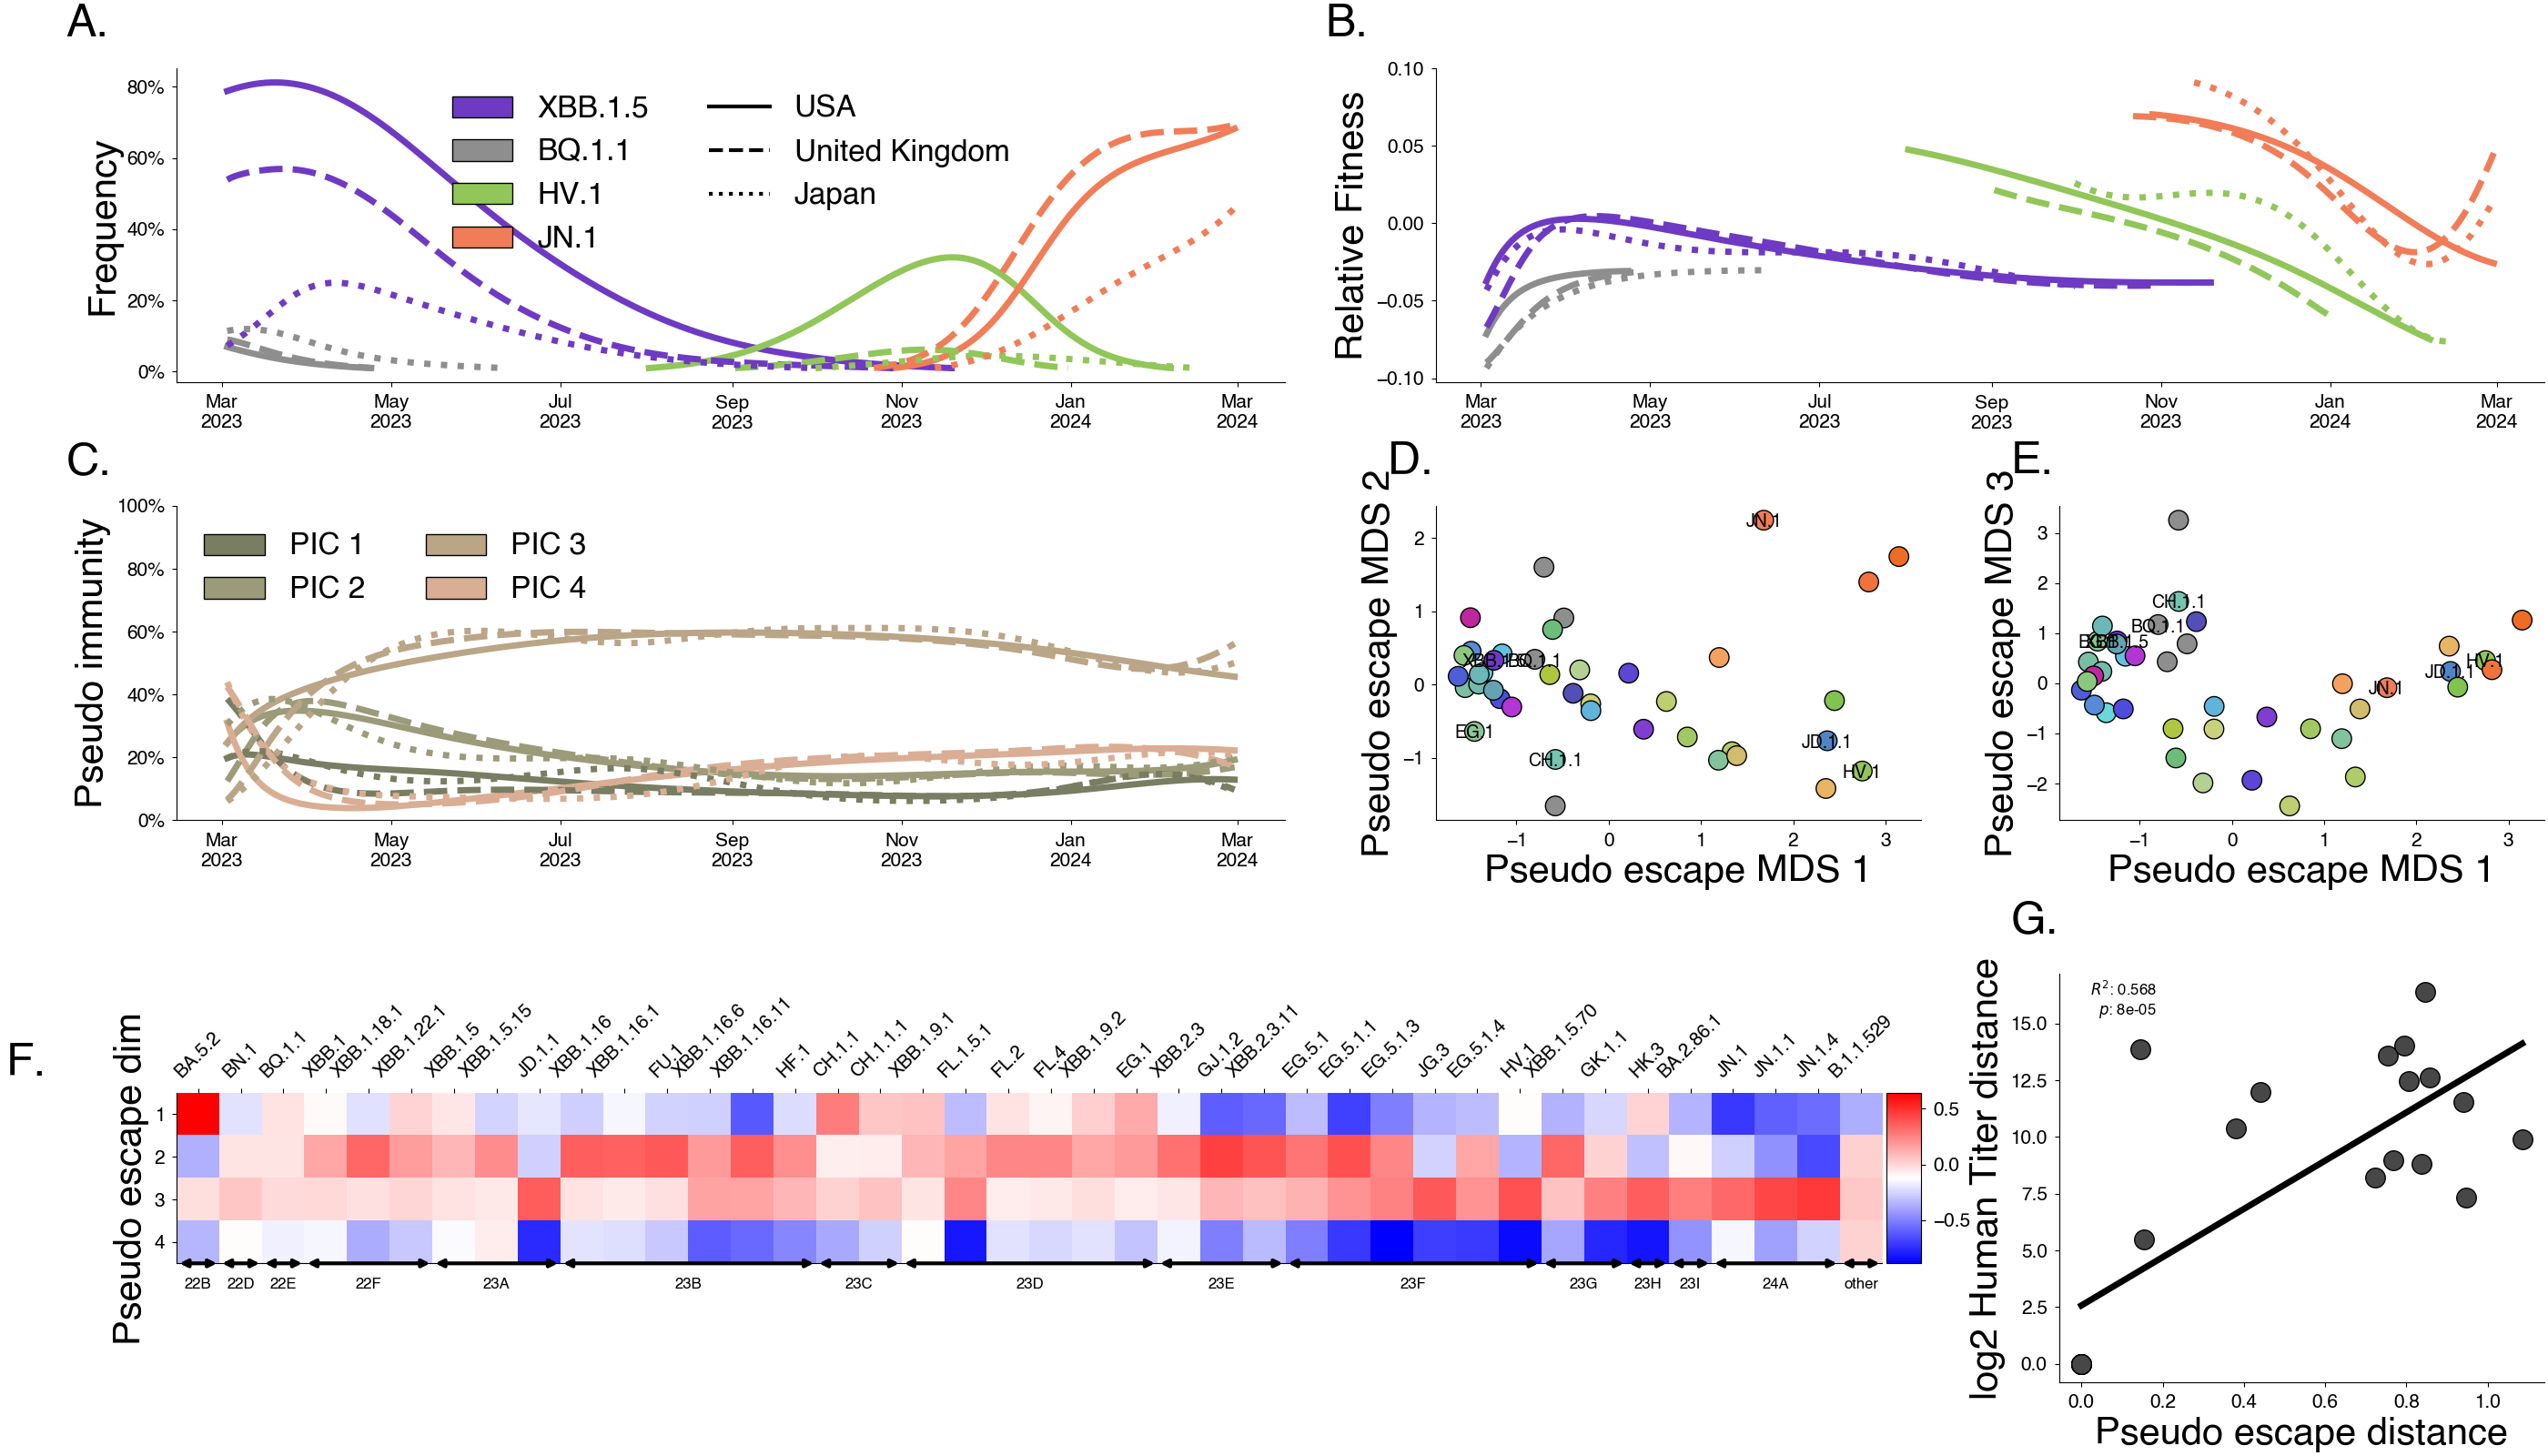
\includegraphics[width=1.0\textwidth=0.01]{./supplementary_figures/latent_immune_4_dims.png}
    \caption{
      \textbf{Latent factor model. $D=4$}
    }
    \label{fig:latent_factor_4}
\end{figure}

\begin{figure}[t!]
    \centering
    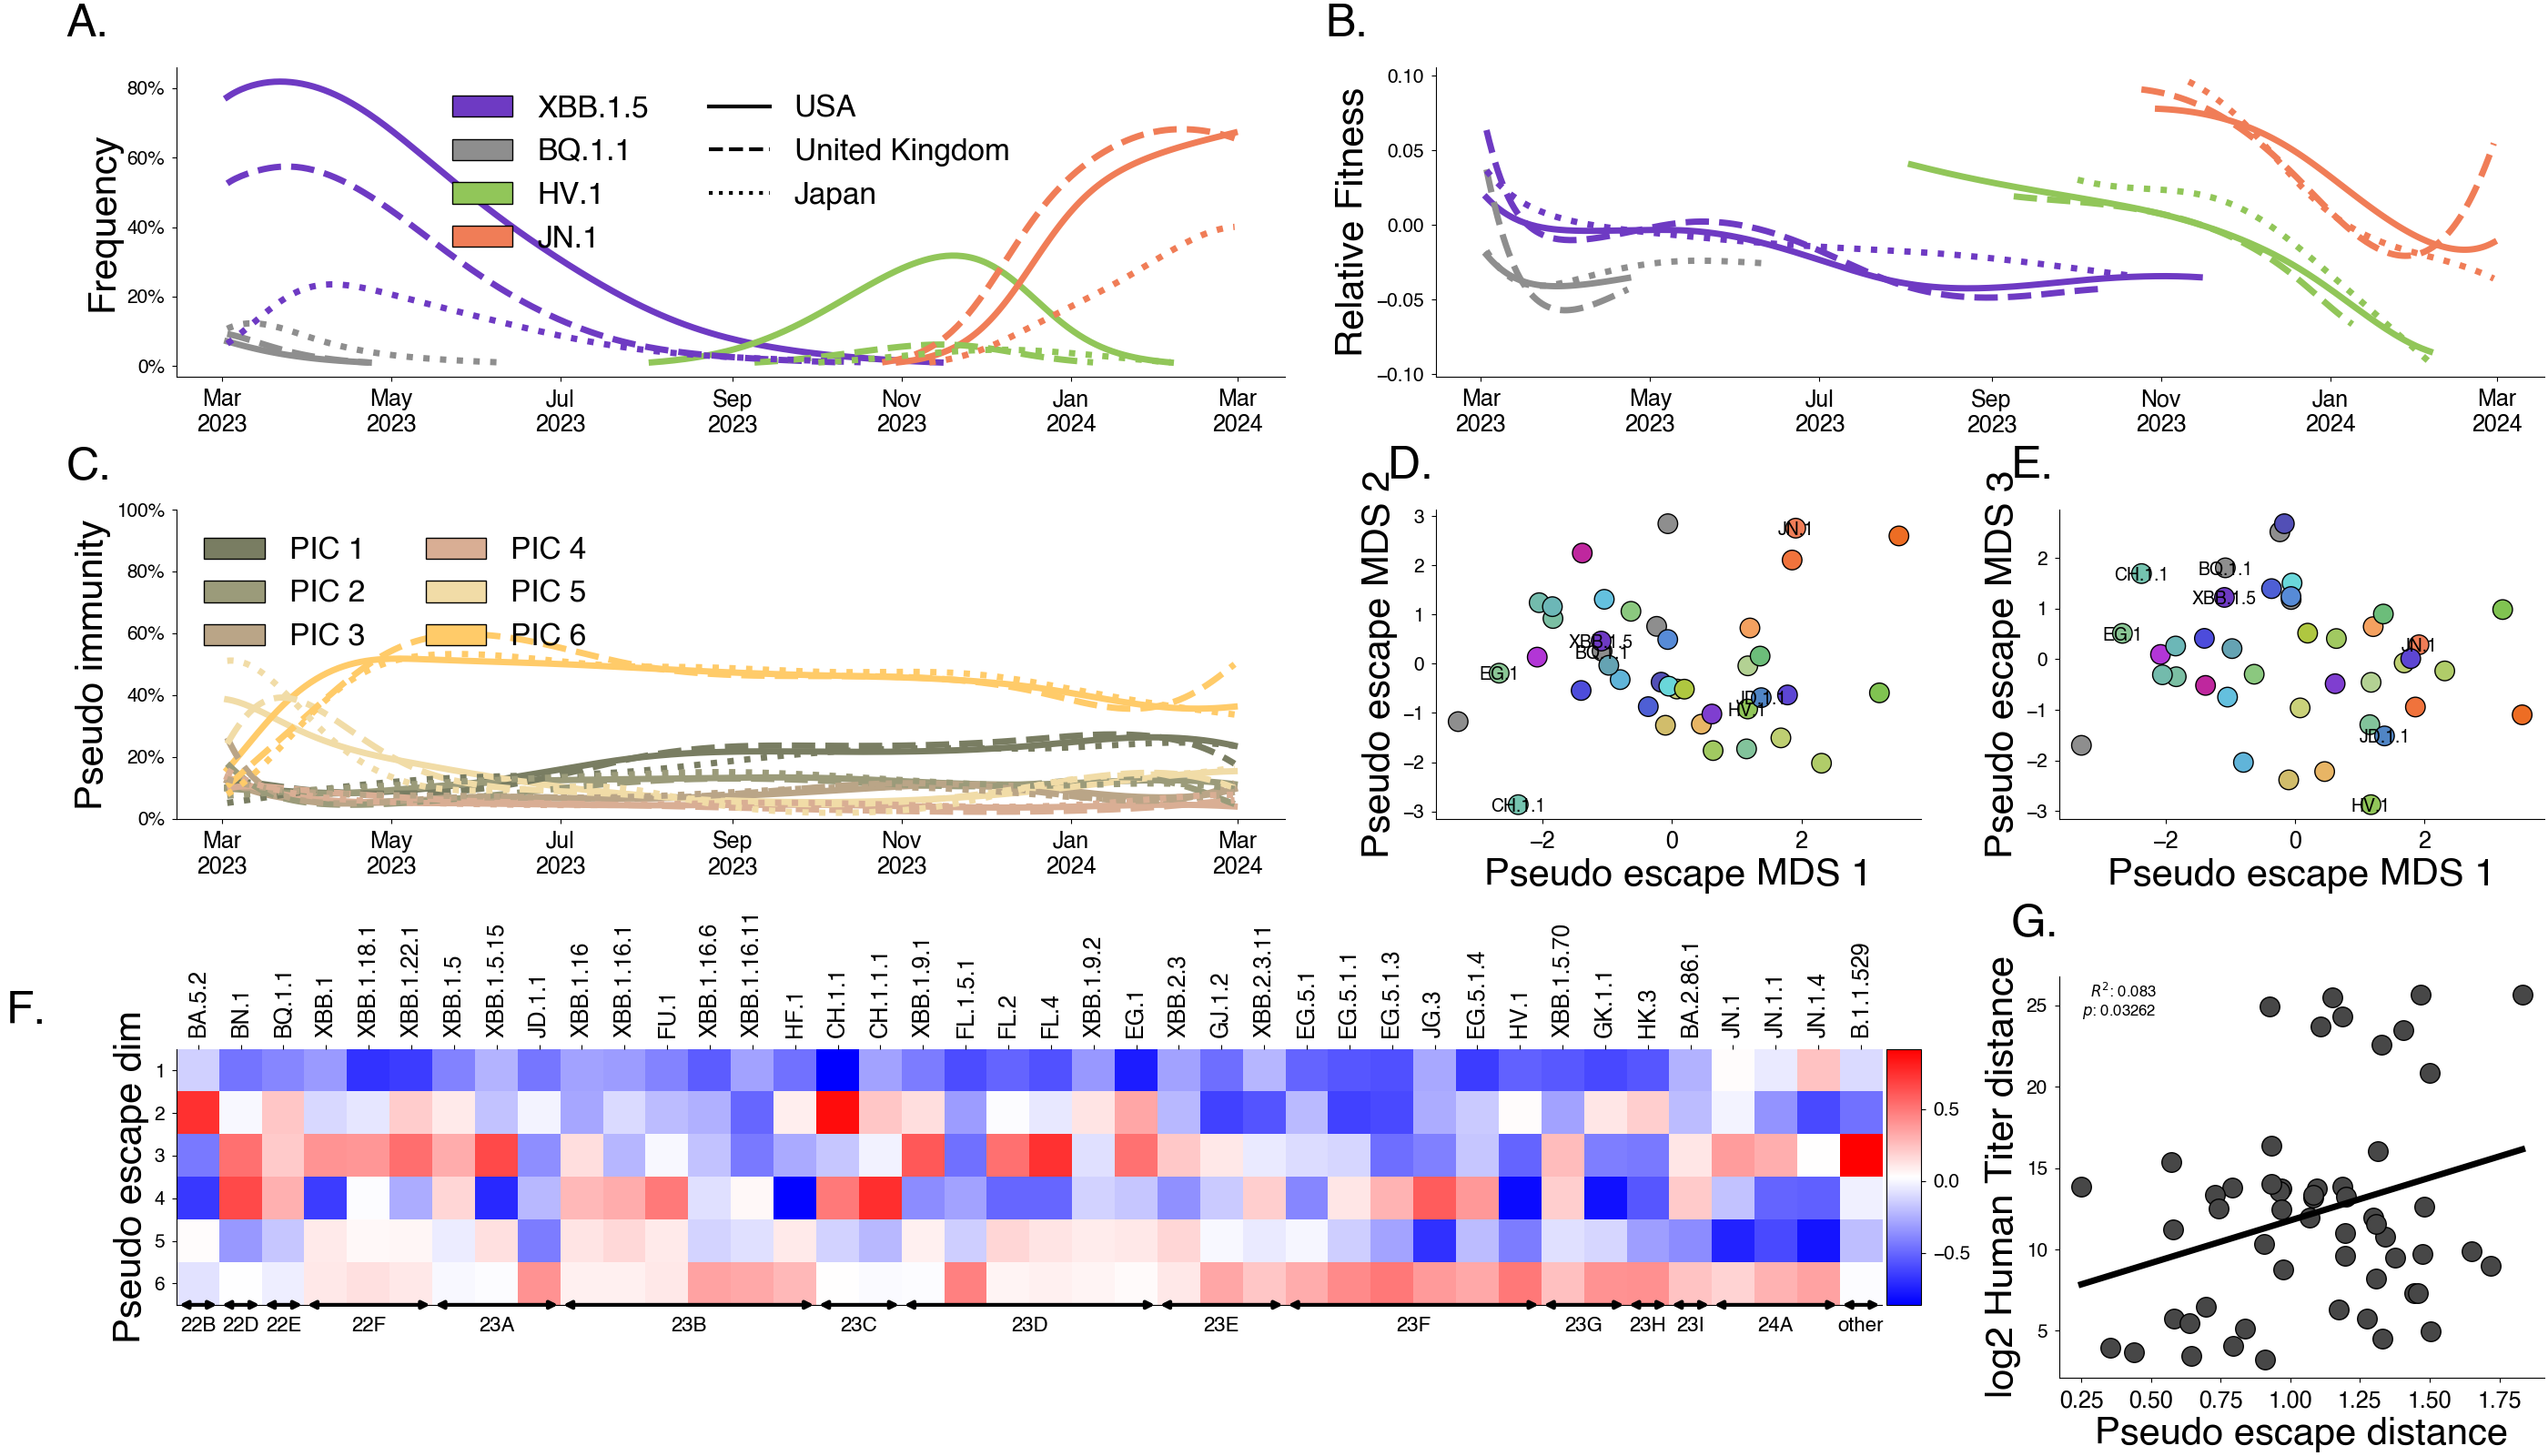
\includegraphics[width=1.0\textwidth=0.01]{./supplementary_figures/latent_immune_6_dims.png}
    \caption{
      \textbf{Latent factor model. $D=6$}
    }
    \label{fig:latent_factor_6}
\end{figure}

\begin{figure}[t!]
    \centering
    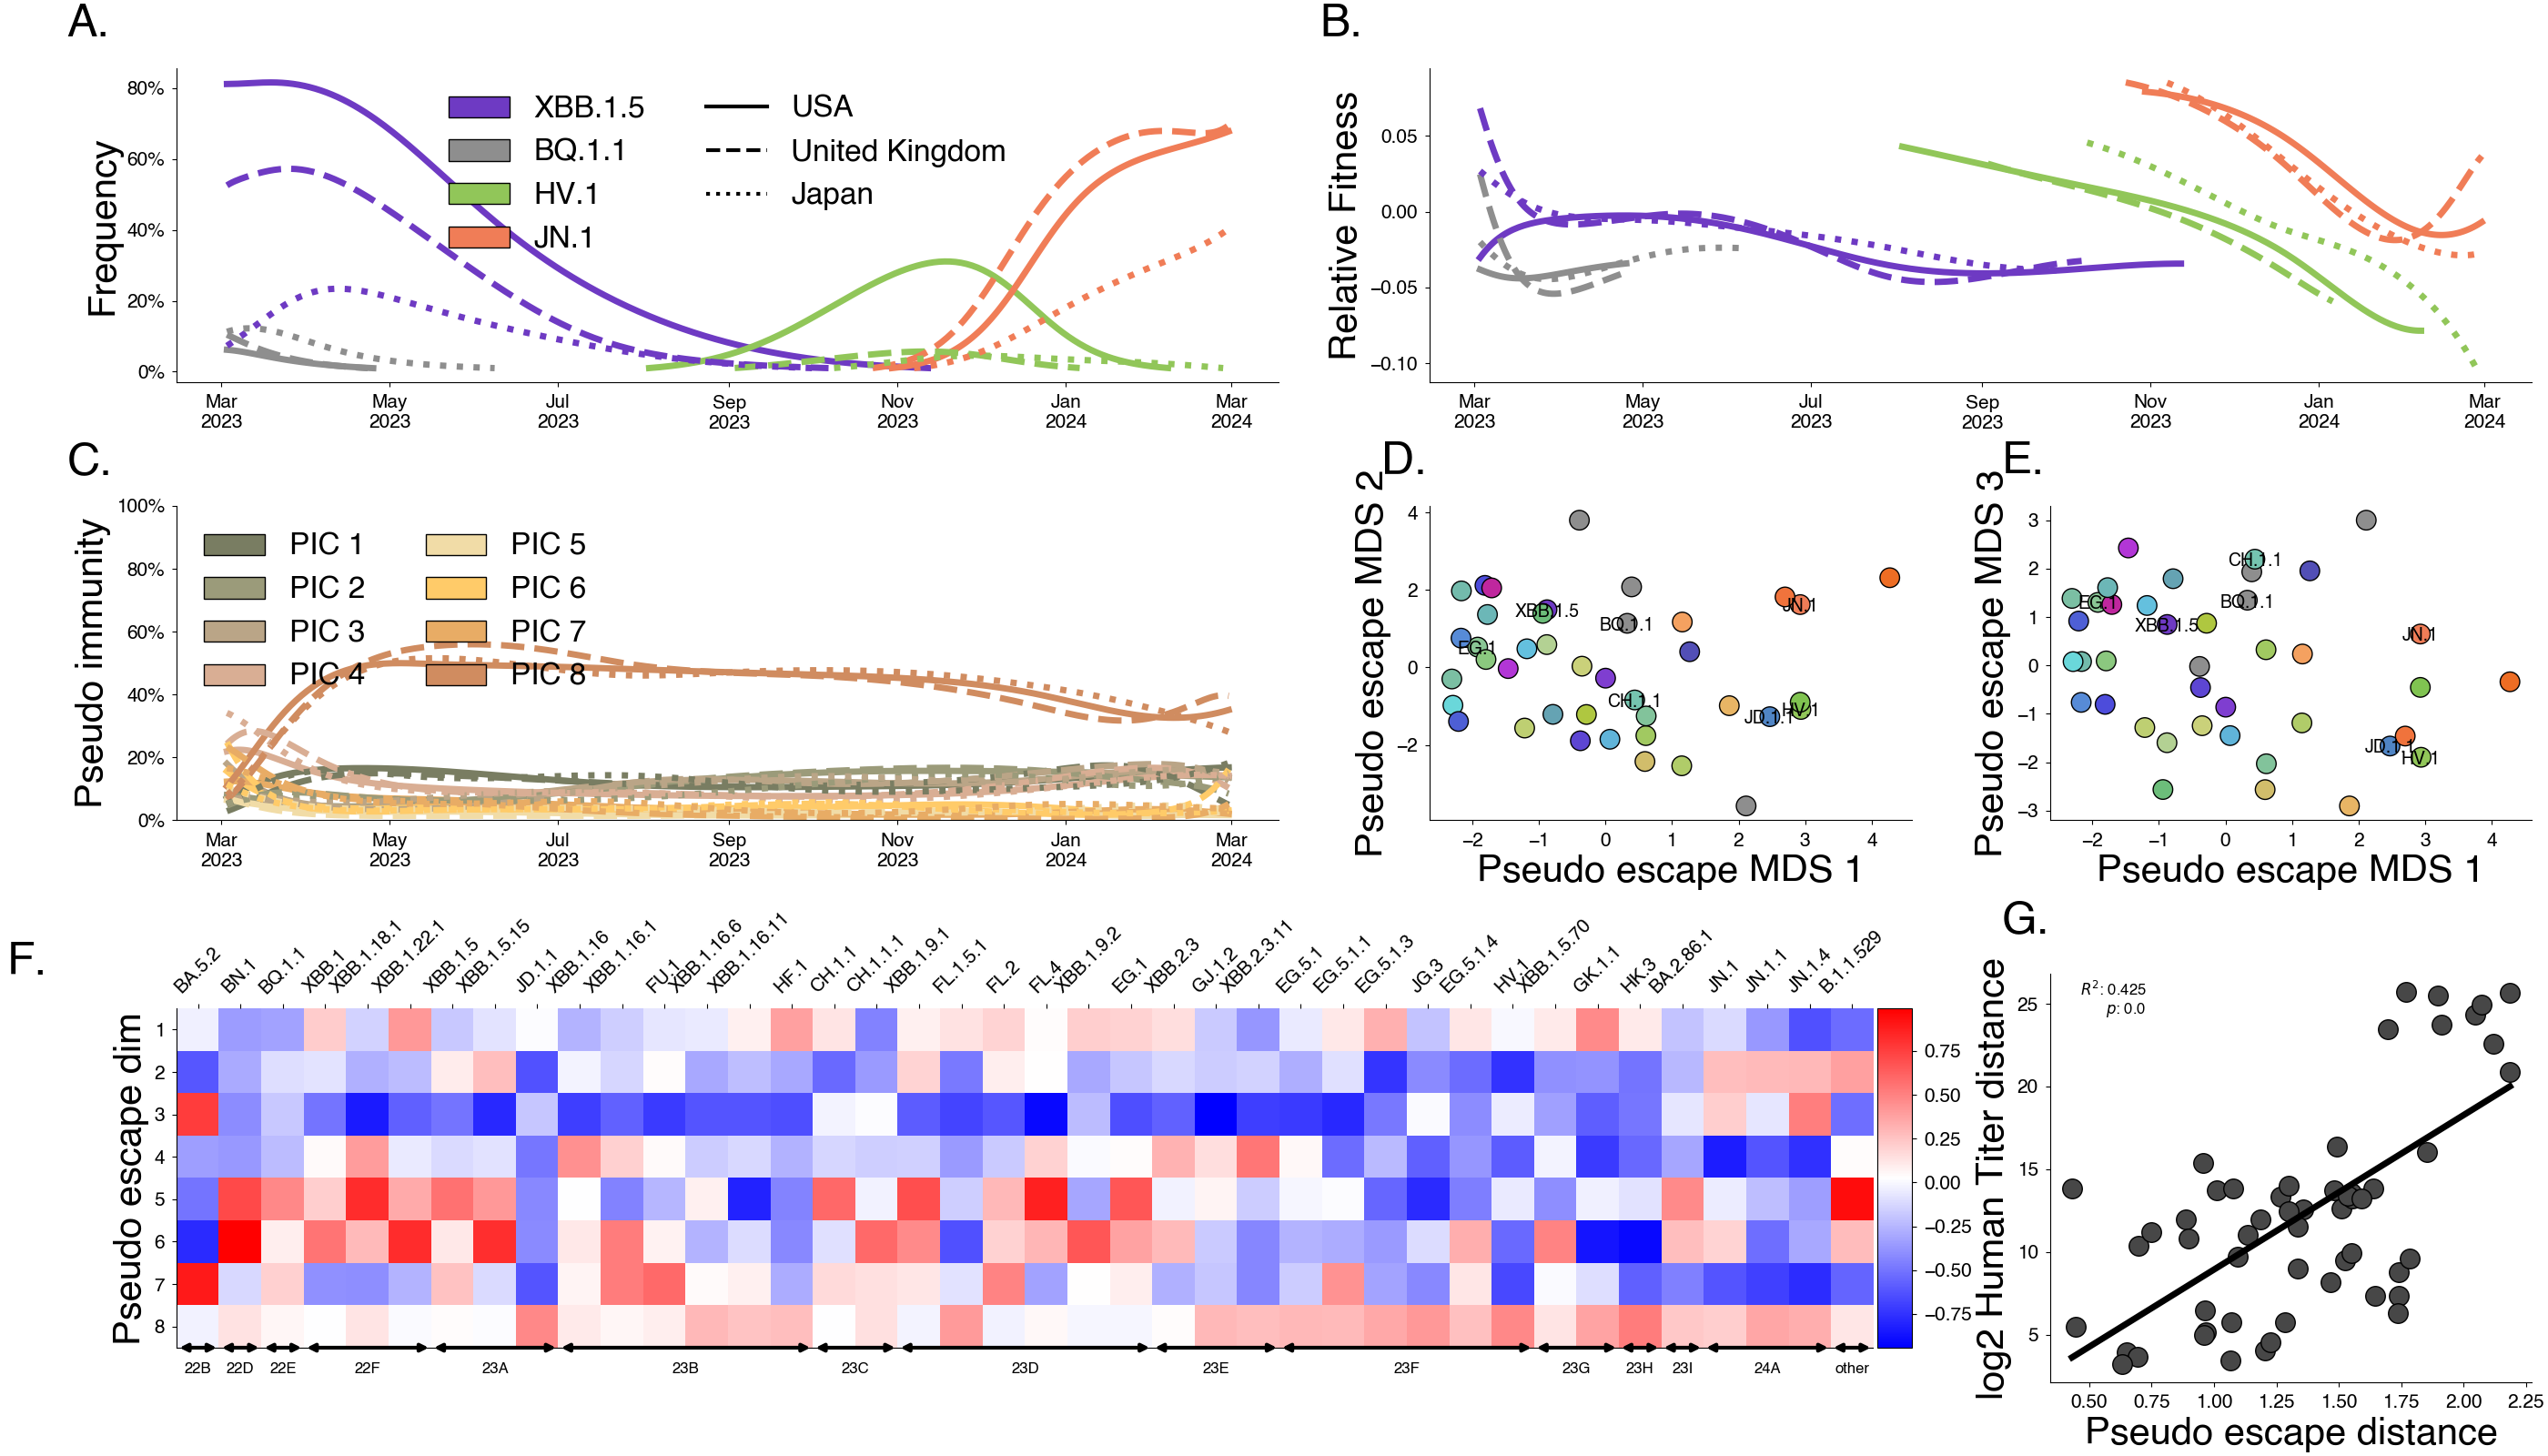
\includegraphics[width=1.0\textwidth=0.01]{./supplementary_figures/latent_immune_8_dims.png}
    \caption{
      \textbf{Latent factor model. $D=8$}
    }
    \label{fig:latent_factor_8}
\end{figure}

\begin{figure}[t!]
    \centering
    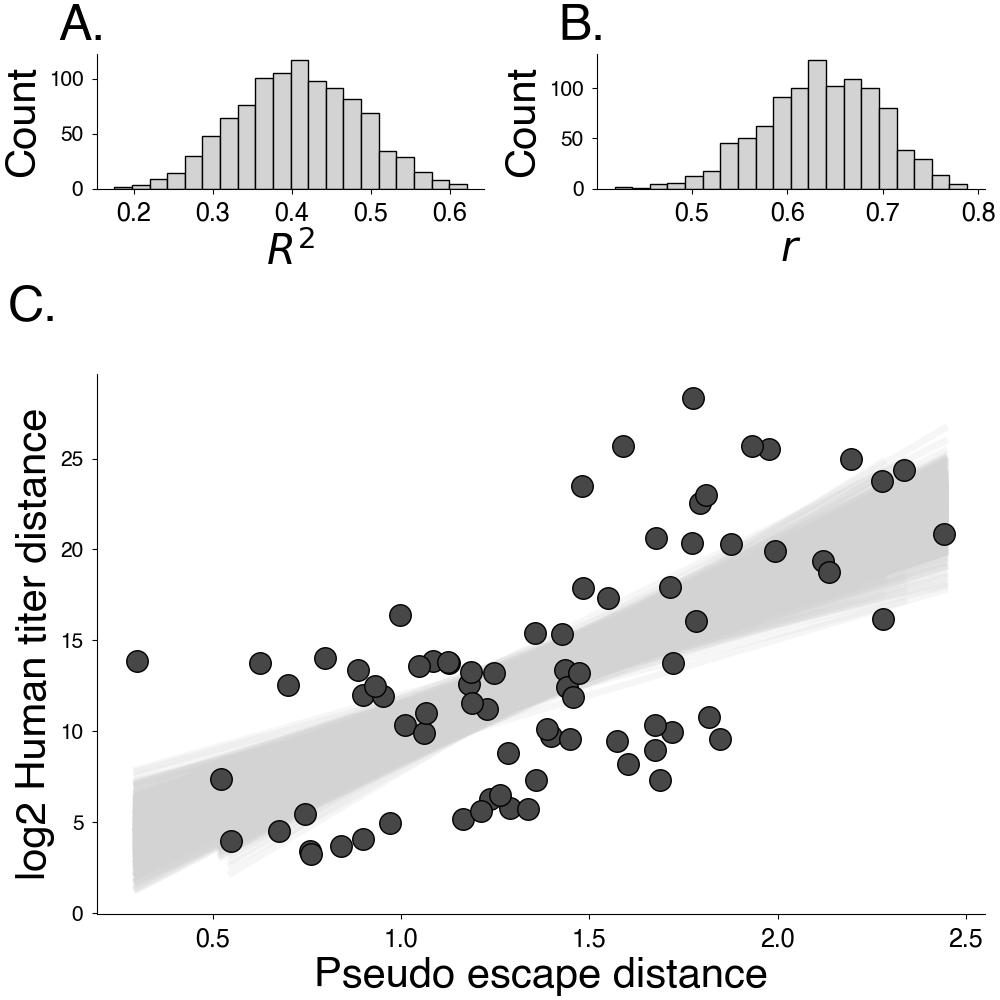
\includegraphics[width=1.0\textwidth=0.01]{./supplementary_figures/pseudo_escape_titer_correlation_bootstrap.png}
    \caption{
        \textbf{Bootstrapping pseudo-immune distance and human titer distance analysis ($N_{\text{replicate}}=1,000$}).
    }
    \label{fig:latent_immune_bootstrap}
\end{figure}

\begin{figure}[t!]
    \centering
    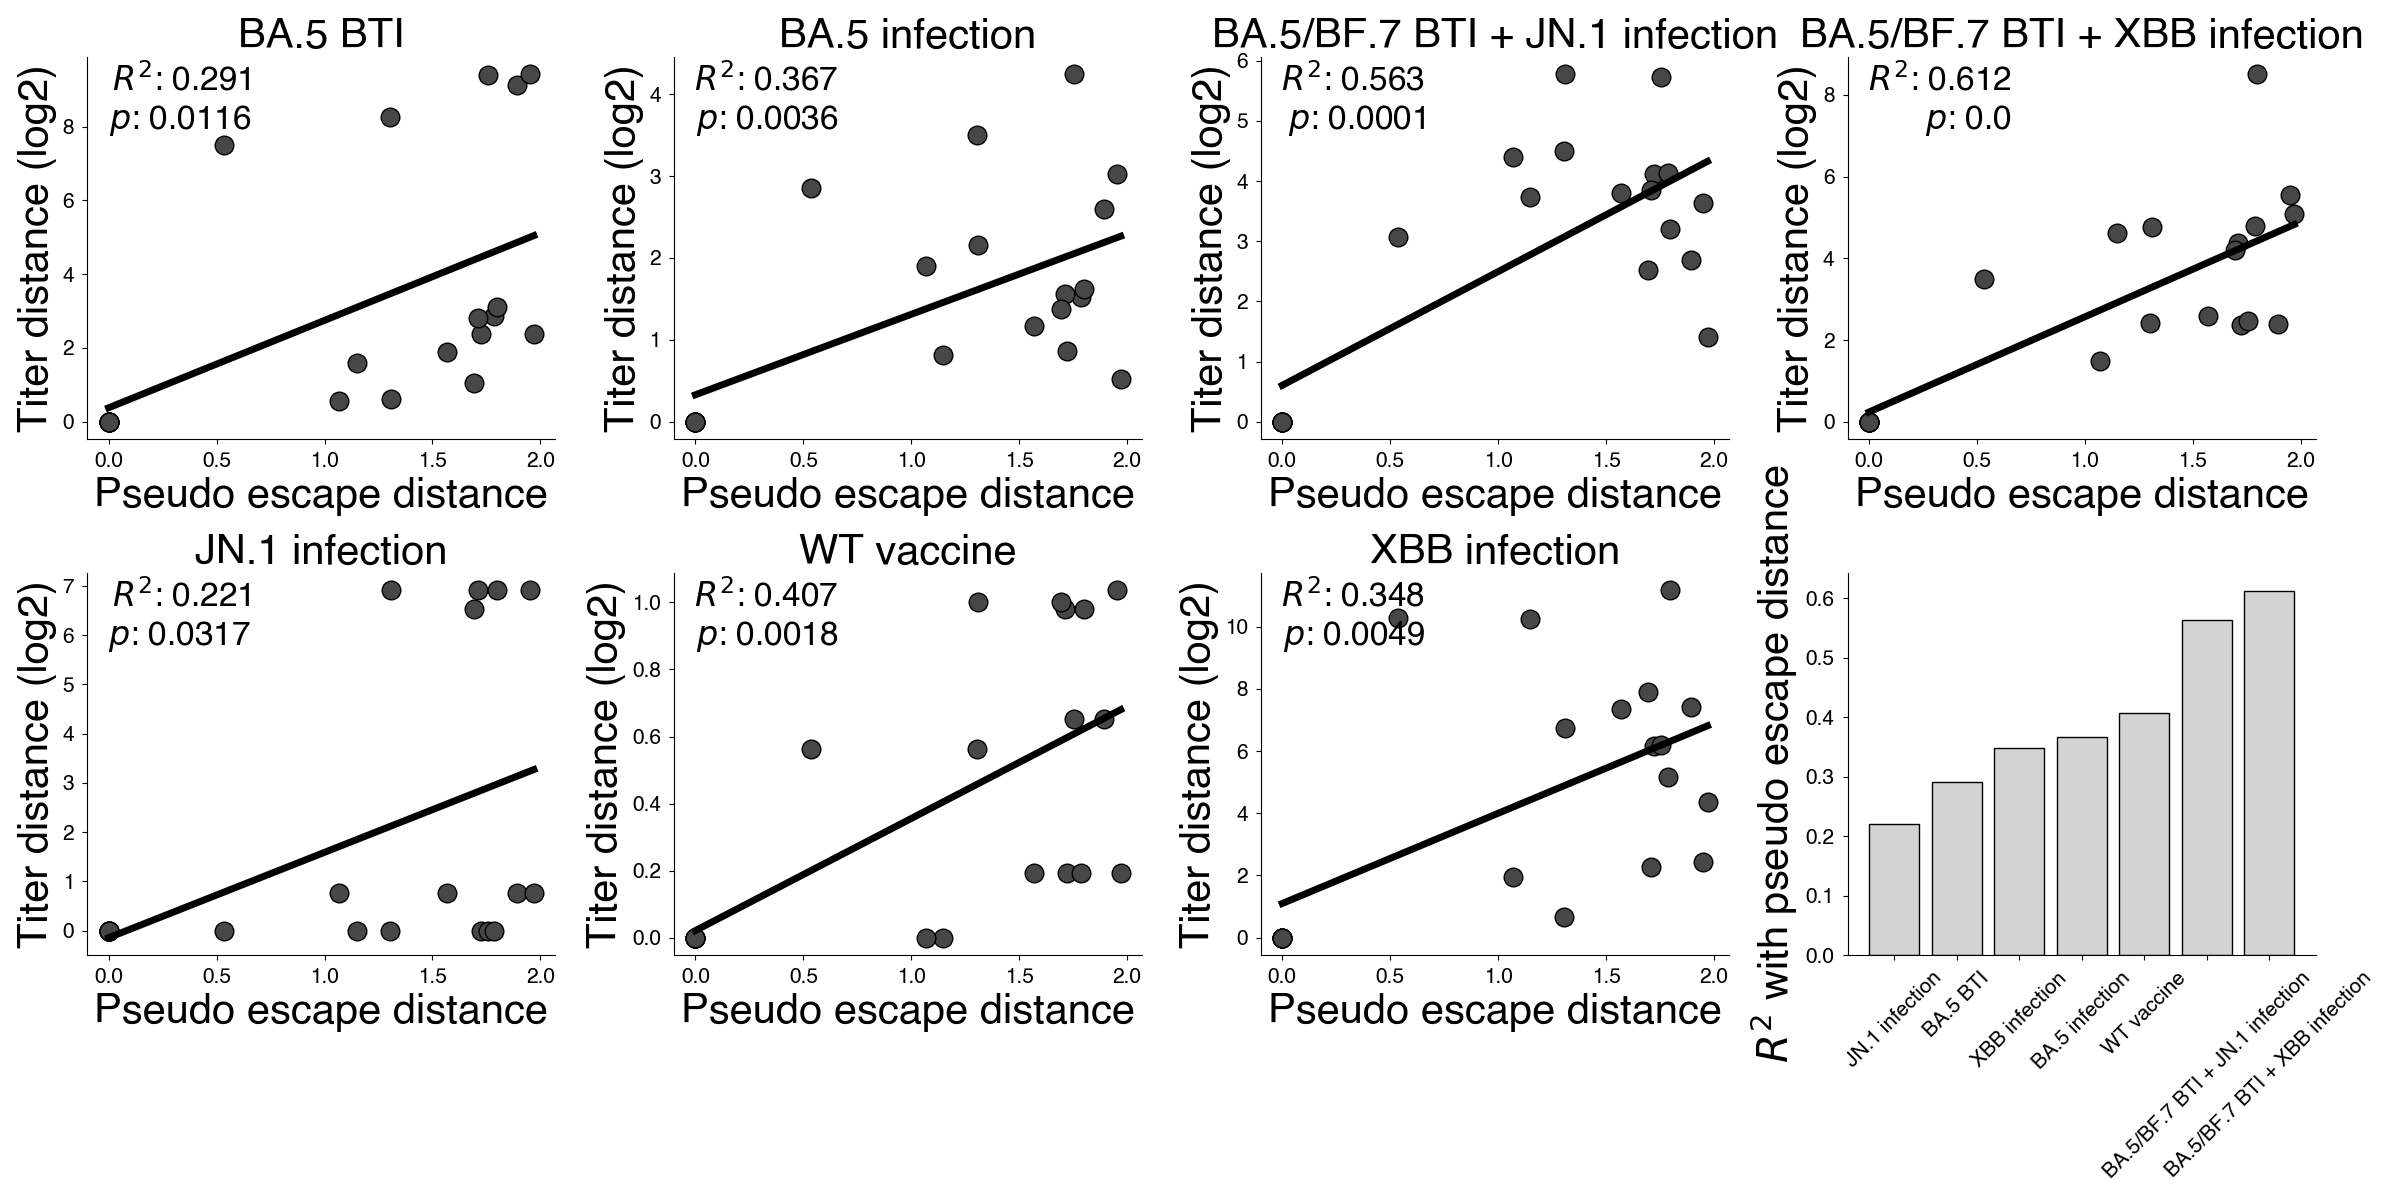
\includegraphics[width=1.0\textwidth=0.01]{./supplementary_figures/titer_pseudo_escape_distance_by_group.png}
    \caption{
        \textbf{Comparing pseudo-escape distance and titer distance between exposure groups.}
    }
    \label{fig:titer_distance_correlations_by_group}
\end{figure}



\end{document}
